\documentclass[twoside]{book}

% Packages required by doxygen
\usepackage{fixltx2e}
\usepackage{calc}
\usepackage{doxygen}
\usepackage[export]{adjustbox} % also loads graphicx
\usepackage{graphicx}
\usepackage[utf8]{inputenc}
\usepackage{makeidx}
\usepackage{multicol}
\usepackage{multirow}
\PassOptionsToPackage{warn}{textcomp}
\usepackage{textcomp}
\usepackage[nointegrals]{wasysym}
\usepackage[table]{xcolor}

% Font selection
\usepackage[T1]{fontenc}
\usepackage[scaled=.90]{helvet}
\usepackage{courier}
\usepackage{amssymb}
\usepackage{sectsty}
\renewcommand{\familydefault}{\sfdefault}
\allsectionsfont{%
  \fontseries{bc}\selectfont%
  \color{darkgray}%
}
\renewcommand{\DoxyLabelFont}{%
  \fontseries{bc}\selectfont%
  \color{darkgray}%
}
\newcommand{\+}{\discretionary{\mbox{\scriptsize$\hookleftarrow$}}{}{}}

% Page & text layout
\usepackage{geometry}
\geometry{%
  a4paper,%
  top=2.5cm,%
  bottom=2.5cm,%
  left=2.5cm,%
  right=2.5cm%
}
\tolerance=750
\hfuzz=15pt
\hbadness=750
\setlength{\emergencystretch}{15pt}
\setlength{\parindent}{0cm}
\setlength{\parskip}{3ex plus 2ex minus 2ex}
\makeatletter
\renewcommand{\paragraph}{%
  \@startsection{paragraph}{4}{0ex}{-1.0ex}{1.0ex}{%
    \normalfont\normalsize\bfseries\SS@parafont%
  }%
}
\renewcommand{\subparagraph}{%
  \@startsection{subparagraph}{5}{0ex}{-1.0ex}{1.0ex}{%
    \normalfont\normalsize\bfseries\SS@subparafont%
  }%
}
\makeatother

% Headers & footers
\usepackage{fancyhdr}
\pagestyle{fancyplain}
\fancyhead[LE]{\fancyplain{}{\bfseries\thepage}}
\fancyhead[CE]{\fancyplain{}{}}
\fancyhead[RE]{\fancyplain{}{\bfseries\leftmark}}
\fancyhead[LO]{\fancyplain{}{\bfseries\rightmark}}
\fancyhead[CO]{\fancyplain{}{}}
\fancyhead[RO]{\fancyplain{}{\bfseries\thepage}}
\fancyfoot[LE]{\fancyplain{}{}}
\fancyfoot[CE]{\fancyplain{}{}}
\fancyfoot[RE]{\fancyplain{}{\bfseries\scriptsize Generated by Doxygen }}
\fancyfoot[LO]{\fancyplain{}{\bfseries\scriptsize Generated by Doxygen }}
\fancyfoot[CO]{\fancyplain{}{}}
\fancyfoot[RO]{\fancyplain{}{}}
\renewcommand{\footrulewidth}{0.4pt}
\renewcommand{\chaptermark}[1]{%
  \markboth{#1}{}%
}
\renewcommand{\sectionmark}[1]{%
  \markright{\thesection\ #1}%
}

% Indices & bibliography
\usepackage{natbib}
\usepackage[titles]{tocloft}
\setcounter{tocdepth}{3}
\setcounter{secnumdepth}{5}
\makeindex

% Hyperlinks (required, but should be loaded last)
\usepackage{ifpdf}
\ifpdf
  \usepackage[pdftex,pagebackref=true]{hyperref}
\else
  \usepackage[ps2pdf,pagebackref=true]{hyperref}
\fi
\hypersetup{%
  colorlinks=true,%
  linkcolor=blue,%
  citecolor=blue,%
  unicode%
}

% Custom commands
\newcommand{\clearemptydoublepage}{%
  \newpage{\pagestyle{empty}\cleardoublepage}%
}

\usepackage{caption}
\captionsetup{labelsep=space,justification=centering,font={bf},singlelinecheck=off,skip=4pt,position=top}

%===== C O N T E N T S =====

\begin{document}

% Titlepage & ToC
\hypersetup{pageanchor=false,
             bookmarksnumbered=true,
             pdfencoding=unicode
            }
\pagenumbering{alph}
\begin{titlepage}
\vspace*{7cm}
\begin{center}%
{\Large D\+O\+X\+\_\+\+A\+R\+S\+A\+L\+\_\+\+Sources }\\
\vspace*{1cm}
{\large Generated by Doxygen 1.8.12}\\
\end{center}
\end{titlepage}
\clearemptydoublepage
\pagenumbering{roman}
\tableofcontents
\clearemptydoublepage
\pagenumbering{arabic}
\hypersetup{pageanchor=true}

%--- Begin generated contents ---
\chapter{Hierarchical Index}
\section{Class Hierarchy}
This inheritance list is sorted roughly, but not completely, alphabetically\+:\begin{DoxyCompactList}
\item \contentsline{section}{\+\_\+\+A\+R\+S\+A\+L\+\_\+\+F\+T\+W\+\_\+t}{\pageref{struct__ARSAL__FTW__t}}{}
\item \contentsline{section}{\+\_\+\+A\+R\+S\+A\+L\+\_\+\+M\+D5\+\_\+\+Manager\+\_\+t}{\pageref{struct__ARSAL__MD5__Manager__t}}{}
\item $<$C\+B\+Central\+Manager\+Delegate$>$\begin{DoxyCompactList}
\item \contentsline{section}{A\+R\+S\+A\+L\+\_\+\+B\+L\+E\+Manager}{\pageref{interfaceARSAL__BLEManager}}{}
\end{DoxyCompactList}
\item $<$C\+B\+Peripheral\+Delegate$>$\begin{DoxyCompactList}
\item \contentsline{section}{A\+R\+S\+A\+L\+\_\+\+B\+L\+E\+Manager}{\pageref{interfaceARSAL__BLEManager}}{}
\end{DoxyCompactList}
\item \contentsline{section}{C\+B\+U\+U\+ID(String\+Extraction)}{\pageref{categoryCBUUID_07StringExtraction_08}}{}
\item N\+S\+Object\begin{DoxyCompactList}
\item \contentsline{section}{A\+R\+S\+A\+L\+\_\+\+B\+L\+E\+Manager}{\pageref{interfaceARSAL__BLEManager}}{}
\item \contentsline{section}{A\+R\+S\+A\+L\+\_\+\+Central\+Manager}{\pageref{interfaceARSAL__CentralManager}}{}
\item \contentsline{section}{A\+R\+S\+A\+L\+B\+L\+E\+Manager\+Notification}{\pageref{interfaceARSALBLEManagerNotification}}{}
\item \contentsline{section}{A\+R\+S\+A\+L\+B\+L\+E\+Manager\+Notification\+Data}{\pageref{interfaceARSALBLEManagerNotificationData}}{}
\end{DoxyCompactList}
\item $<$N\+S\+Object\+N\+S\+Object$>$\begin{DoxyCompactList}
\item \contentsline{section}{$<$A\+R\+S\+A\+L\+B\+L\+E\+Manager\+Delegate $>$}{\pageref{protocolARSALBLEManagerDelegate_01-p}}{}
\end{DoxyCompactList}
\end{DoxyCompactList}

\chapter{Class Index}
\section{Class List}
Here are the classes, structs, unions and interfaces with brief descriptions\+:\begin{DoxyCompactList}
\item\contentsline{section}{\hyperlink{struct__ARSAL__FTW__t}{\+\_\+\+A\+R\+S\+A\+L\+\_\+\+F\+T\+W\+\_\+t} \\*A\+R\+S\+A\+L\+\_\+\+F\+T\+W\+\_\+t structure equal to \char`\"{}struct F\+T\+W\char`\"{} }{\pageref{struct__ARSAL__FTW__t}}{}
\item\contentsline{section}{\hyperlink{struct__ARSAL__MD5__Manager__t}{\+\_\+\+A\+R\+S\+A\+L\+\_\+\+M\+D5\+\_\+\+Manager\+\_\+t} \\*M\+D5 Manager structure }{\pageref{struct__ARSAL__MD5__Manager__t}}{}
\item\contentsline{section}{\hyperlink{interfaceARSAL__BLEManager}{A\+R\+S\+A\+L\+\_\+\+B\+L\+E\+Manager} }{\pageref{interfaceARSAL__BLEManager}}{}
\item\contentsline{section}{\hyperlink{interfaceARSAL__CentralManager}{A\+R\+S\+A\+L\+\_\+\+Central\+Manager} }{\pageref{interfaceARSAL__CentralManager}}{}
\item\contentsline{section}{\hyperlink{protocolARSALBLEManagerDelegate_01-p}{$<$\+A\+R\+S\+A\+L\+B\+L\+E\+Manager\+Delegate $>$} }{\pageref{protocolARSALBLEManagerDelegate_01-p}}{}
\item\contentsline{section}{\hyperlink{interfaceARSALBLEManagerNotification}{A\+R\+S\+A\+L\+B\+L\+E\+Manager\+Notification} }{\pageref{interfaceARSALBLEManagerNotification}}{}
\item\contentsline{section}{\hyperlink{interfaceARSALBLEManagerNotificationData}{A\+R\+S\+A\+L\+B\+L\+E\+Manager\+Notification\+Data} }{\pageref{interfaceARSALBLEManagerNotificationData}}{}
\item\contentsline{section}{\hyperlink{categoryCBUUID_07StringExtraction_08}{C\+B\+U\+U\+I\+D(\+String\+Extraction)} }{\pageref{categoryCBUUID_07StringExtraction_08}}{}
\end{DoxyCompactList}

\chapter{File Index}
\section{File List}
Here is a list of all files with brief descriptions\+:\begin{DoxyCompactList}
\item\contentsline{section}{\hyperlink{ARSAL_8h}{A\+R\+S\+A\+L.\+h} \\*Library global header for lib\+A\+R\+S\+AL }{\pageref{ARSAL_8h}}{}
\item\contentsline{section}{\hyperlink{ARSAL__BLEManager_8h}{A\+R\+S\+A\+L\+\_\+\+B\+L\+E\+Manager.\+h} \\*Private headers of B\+LE manager allow to use Bluetooth low energy api\textquotesingle{}s }{\pageref{ARSAL__BLEManager_8h}}{}
\item\contentsline{section}{\hyperlink{ARSAL__CentralManager_8h}{A\+R\+S\+A\+L\+\_\+\+Central\+Manager.\+h} }{\pageref{ARSAL__CentralManager_8h}}{}
\item\contentsline{section}{\hyperlink{ARSAL__Endianness_8h}{A\+R\+S\+A\+L\+\_\+\+Endianness.\+h} \\*This file contains headers about endianness abstraction layer }{\pageref{ARSAL__Endianness_8h}}{}
\item\contentsline{section}{\hyperlink{ARSAL__Error_8h}{A\+R\+S\+A\+L\+\_\+\+Error.\+h} }{\pageref{ARSAL__Error_8h}}{}
\item\contentsline{section}{\hyperlink{ARSAL__Ftw_8h}{A\+R\+S\+A\+L\+\_\+\+Ftw.\+h} \\*Lib\+A\+R\+S\+AL Ftw header file }{\pageref{ARSAL__Ftw_8h}}{}
\item\contentsline{section}{\hyperlink{ARSAL__MD5__Manager_8h}{A\+R\+S\+A\+L\+\_\+\+M\+D5\+\_\+\+Manager.\+h} }{\pageref{ARSAL__MD5__Manager_8h}}{}
\item\contentsline{section}{\hyperlink{ARSAL__Mutex_8h}{A\+R\+S\+A\+L\+\_\+\+Mutex.\+h} \\*This file contains headers about mutex abstraction layer }{\pageref{ARSAL__Mutex_8h}}{}
\item\contentsline{section}{\hyperlink{ARSAL__Print_8h}{A\+R\+S\+A\+L\+\_\+\+Print.\+h} \\*This file contains headers about debug print abstraction layer }{\pageref{ARSAL__Print_8h}}{}
\item\contentsline{section}{\hyperlink{ARSAL__Sem_8h}{A\+R\+S\+A\+L\+\_\+\+Sem.\+h} \\*This file contains headers about semaphore abstraction layer }{\pageref{ARSAL__Sem_8h}}{}
\item\contentsline{section}{\hyperlink{ARSAL__Singleton_8h}{A\+R\+S\+A\+L\+\_\+\+Singleton.\+h} \\*Headers to define singletons }{\pageref{ARSAL__Singleton_8h}}{}
\item\contentsline{section}{\hyperlink{ARSAL__Socket_8h}{A\+R\+S\+A\+L\+\_\+\+Socket.\+h} \\*This file contains headers about socket abstraction layer }{\pageref{ARSAL__Socket_8h}}{}
\item\contentsline{section}{\hyperlink{ARSAL__Thread_8h}{A\+R\+S\+A\+L\+\_\+\+Thread.\+h} \\*This file contains headers about thread abstraction layer }{\pageref{ARSAL__Thread_8h}}{}
\item\contentsline{section}{\hyperlink{ARSAL__Time_8h}{A\+R\+S\+A\+L\+\_\+\+Time.\+h} \\*This file contains headers about time abstraction layer }{\pageref{ARSAL__Time_8h}}{}
\end{DoxyCompactList}

\chapter{Class Documentation}
\hypertarget{classARSAL__BLEManager}{}\section{A\+R\+S\+A\+L\+\_\+\+B\+L\+E\+Manager Class Reference}
\label{classARSAL__BLEManager}\index{A\+R\+S\+A\+L\+\_\+\+B\+L\+E\+Manager@{A\+R\+S\+A\+L\+\_\+\+B\+L\+E\+Manager}}


The documentation for this class was generated from the following file\+:\begin{DoxyCompactItemize}
\item 
\hyperlink{ARSAL__BLEManager_8m}{A\+R\+S\+A\+L\+\_\+\+B\+L\+E\+Manager.\+m}\end{DoxyCompactItemize}

\hypertarget{categoryARSAL__BLEManager_07_08}{}\section{A\+R\+S\+A\+L\+\_\+\+B\+L\+E\+Manager() Category Reference}
\label{categoryARSAL__BLEManager_07_08}\index{A\+R\+S\+A\+L\+\_\+\+B\+L\+E\+Manager()@{A\+R\+S\+A\+L\+\_\+\+B\+L\+E\+Manager()}}
\subsection*{Instance Methods}
\begin{DoxyCompactItemize}
\item 
(void) -\/ \hyperlink{categoryARSAL__BLEManager_07_08_a114ff594e83a767cd582b77cdc25d7f0}{A\+R\+S\+A\+L\+\_\+\+B\+L\+E\+Manager\+\_\+\+Init}
\end{DoxyCompactItemize}
\subsection*{Properties}
\begin{DoxyCompactItemize}
\item 
e\+A\+R\+S\+A\+L\+\_\+\+E\+R\+R\+OR \hyperlink{categoryARSAL__BLEManager_07_08_afb7dca42e2a5996dcfc6d0eeea84ce14}{discover\+Services\+Error}
\item 
e\+A\+R\+S\+A\+L\+\_\+\+E\+R\+R\+OR \hyperlink{categoryARSAL__BLEManager_07_08_afaa6de70a23b7a5dd26a7c788c0ec135}{discover\+Characteristics\+Error}
\item 
e\+A\+R\+S\+A\+L\+\_\+\+E\+R\+R\+OR \hyperlink{categoryARSAL__BLEManager_07_08_ad4bfa8fea63cbffff5711e503f902a21}{configuration\+Characteristic\+Error}
\item 
e\+A\+R\+S\+A\+L\+\_\+\+E\+R\+R\+OR \hyperlink{categoryARSAL__BLEManager_07_08_a2a57520b14dc0500d5f77b4d056c6d43}{write\+Characteristic\+Error}
\item 
B\+O\+OL \hyperlink{categoryARSAL__BLEManager_07_08_a9545df8b76da87a8a4032d7b3b4d424d}{ask\+Disconnection}
\item 
B\+O\+OL \hyperlink{categoryARSAL__BLEManager_07_08_a8b0c53009ab15317c3cf9e1e178f14b0}{is\+Discovering\+Services}
\item 
B\+O\+OL \hyperlink{categoryARSAL__BLEManager_07_08_ab159618d9d76b98cfaa53cf66820cefb}{is\+Discovering\+Characteristics}
\item 
B\+O\+OL \hyperlink{categoryARSAL__BLEManager_07_08_a3124cd1734adfa93b1226c8ac222423f}{is\+Configuring\+Characteristics}
\item 
B\+O\+OL \hyperlink{categoryARSAL__BLEManager_07_08_a8268a431f84c1cf80683dcd49d5e69e7}{is\+Writing\+Characteristic}
\item 
N\+S\+Mutable\+Dictionary $\ast$ \hyperlink{categoryARSAL__BLEManager_07_08_a7325b966cd388be3e1af8da9a5dcf877}{registered\+Notification\+Characteristics}
\item 
A\+R\+S\+A\+L\+\_\+\+Mutex\+\_\+t \hyperlink{categoryARSAL__BLEManager_07_08_aaef95045d3088929af2f3efb3c5907ff}{reg\+Not\+Characteristics\+Mutex}
\end{DoxyCompactItemize}


\subsection{Method Documentation}
\hypertarget{categoryARSAL__BLEManager_07_08_a114ff594e83a767cd582b77cdc25d7f0}{}\label{categoryARSAL__BLEManager_07_08_a114ff594e83a767cd582b77cdc25d7f0} 
\index{A\+R\+S\+A\+L\+\_\+\+B\+L\+E\+Manager()@{A\+R\+S\+A\+L\+\_\+\+B\+L\+E\+Manager()}!A\+R\+S\+A\+L\+\_\+\+B\+L\+E\+Manager\+\_\+\+Init@{A\+R\+S\+A\+L\+\_\+\+B\+L\+E\+Manager\+\_\+\+Init}}
\index{A\+R\+S\+A\+L\+\_\+\+B\+L\+E\+Manager\+\_\+\+Init@{A\+R\+S\+A\+L\+\_\+\+B\+L\+E\+Manager\+\_\+\+Init}!A\+R\+S\+A\+L\+\_\+\+B\+L\+E\+Manager()@{A\+R\+S\+A\+L\+\_\+\+B\+L\+E\+Manager()}}
\subsubsection{\texorpdfstring{A\+R\+S\+A\+L\+\_\+\+B\+L\+E\+Manager\+\_\+\+Init()}{ARSAL\_BLEManager\_Init()}}
{\footnotesize\ttfamily -\/ (void) A\+R\+S\+A\+L\+\_\+\+B\+L\+E\+Manager\+\_\+\+Init \begin{DoxyParamCaption}{ }\end{DoxyParamCaption}}



\subsection{Property Documentation}
\hypertarget{categoryARSAL__BLEManager_07_08_a9545df8b76da87a8a4032d7b3b4d424d}{}\label{categoryARSAL__BLEManager_07_08_a9545df8b76da87a8a4032d7b3b4d424d} 
\index{A\+R\+S\+A\+L\+\_\+\+B\+L\+E\+Manager()@{A\+R\+S\+A\+L\+\_\+\+B\+L\+E\+Manager()}!ask\+Disconnection@{ask\+Disconnection}}
\index{ask\+Disconnection@{ask\+Disconnection}!A\+R\+S\+A\+L\+\_\+\+B\+L\+E\+Manager()@{A\+R\+S\+A\+L\+\_\+\+B\+L\+E\+Manager()}}
\subsubsection{\texorpdfstring{ask\+Disconnection}{askDisconnection}}
{\footnotesize\ttfamily -\/ (B\+O\+OL) ask\+Disconnection\hspace{0.3cm}{\ttfamily [read]}, {\ttfamily [write]}, {\ttfamily [nonatomic]}, {\ttfamily [assign]}}

\hypertarget{categoryARSAL__BLEManager_07_08_ad4bfa8fea63cbffff5711e503f902a21}{}\label{categoryARSAL__BLEManager_07_08_ad4bfa8fea63cbffff5711e503f902a21} 
\index{A\+R\+S\+A\+L\+\_\+\+B\+L\+E\+Manager()@{A\+R\+S\+A\+L\+\_\+\+B\+L\+E\+Manager()}!configuration\+Characteristic\+Error@{configuration\+Characteristic\+Error}}
\index{configuration\+Characteristic\+Error@{configuration\+Characteristic\+Error}!A\+R\+S\+A\+L\+\_\+\+B\+L\+E\+Manager()@{A\+R\+S\+A\+L\+\_\+\+B\+L\+E\+Manager()}}
\subsubsection{\texorpdfstring{configuration\+Characteristic\+Error}{configurationCharacteristicError}}
{\footnotesize\ttfamily -\/ (e\+A\+R\+S\+A\+L\+\_\+\+E\+R\+R\+OR) configuration\+Characteristic\+Error\hspace{0.3cm}{\ttfamily [read]}, {\ttfamily [write]}, {\ttfamily [nonatomic]}, {\ttfamily [assign]}}

\hypertarget{categoryARSAL__BLEManager_07_08_afaa6de70a23b7a5dd26a7c788c0ec135}{}\label{categoryARSAL__BLEManager_07_08_afaa6de70a23b7a5dd26a7c788c0ec135} 
\index{A\+R\+S\+A\+L\+\_\+\+B\+L\+E\+Manager()@{A\+R\+S\+A\+L\+\_\+\+B\+L\+E\+Manager()}!discover\+Characteristics\+Error@{discover\+Characteristics\+Error}}
\index{discover\+Characteristics\+Error@{discover\+Characteristics\+Error}!A\+R\+S\+A\+L\+\_\+\+B\+L\+E\+Manager()@{A\+R\+S\+A\+L\+\_\+\+B\+L\+E\+Manager()}}
\subsubsection{\texorpdfstring{discover\+Characteristics\+Error}{discoverCharacteristicsError}}
{\footnotesize\ttfamily -\/ (e\+A\+R\+S\+A\+L\+\_\+\+E\+R\+R\+OR) discover\+Characteristics\+Error\hspace{0.3cm}{\ttfamily [read]}, {\ttfamily [write]}, {\ttfamily [nonatomic]}, {\ttfamily [assign]}}

\hypertarget{categoryARSAL__BLEManager_07_08_afb7dca42e2a5996dcfc6d0eeea84ce14}{}\label{categoryARSAL__BLEManager_07_08_afb7dca42e2a5996dcfc6d0eeea84ce14} 
\index{A\+R\+S\+A\+L\+\_\+\+B\+L\+E\+Manager()@{A\+R\+S\+A\+L\+\_\+\+B\+L\+E\+Manager()}!discover\+Services\+Error@{discover\+Services\+Error}}
\index{discover\+Services\+Error@{discover\+Services\+Error}!A\+R\+S\+A\+L\+\_\+\+B\+L\+E\+Manager()@{A\+R\+S\+A\+L\+\_\+\+B\+L\+E\+Manager()}}
\subsubsection{\texorpdfstring{discover\+Services\+Error}{discoverServicesError}}
{\footnotesize\ttfamily -\/ (e\+A\+R\+S\+A\+L\+\_\+\+E\+R\+R\+OR) discover\+Services\+Error\hspace{0.3cm}{\ttfamily [read]}, {\ttfamily [write]}, {\ttfamily [nonatomic]}, {\ttfamily [assign]}}

\hypertarget{categoryARSAL__BLEManager_07_08_a3124cd1734adfa93b1226c8ac222423f}{}\label{categoryARSAL__BLEManager_07_08_a3124cd1734adfa93b1226c8ac222423f} 
\index{A\+R\+S\+A\+L\+\_\+\+B\+L\+E\+Manager()@{A\+R\+S\+A\+L\+\_\+\+B\+L\+E\+Manager()}!is\+Configuring\+Characteristics@{is\+Configuring\+Characteristics}}
\index{is\+Configuring\+Characteristics@{is\+Configuring\+Characteristics}!A\+R\+S\+A\+L\+\_\+\+B\+L\+E\+Manager()@{A\+R\+S\+A\+L\+\_\+\+B\+L\+E\+Manager()}}
\subsubsection{\texorpdfstring{is\+Configuring\+Characteristics}{isConfiguringCharacteristics}}
{\footnotesize\ttfamily -\/ (B\+O\+OL) is\+Configuring\+Characteristics\hspace{0.3cm}{\ttfamily [read]}, {\ttfamily [write]}, {\ttfamily [nonatomic]}, {\ttfamily [assign]}}

\hypertarget{categoryARSAL__BLEManager_07_08_ab159618d9d76b98cfaa53cf66820cefb}{}\label{categoryARSAL__BLEManager_07_08_ab159618d9d76b98cfaa53cf66820cefb} 
\index{A\+R\+S\+A\+L\+\_\+\+B\+L\+E\+Manager()@{A\+R\+S\+A\+L\+\_\+\+B\+L\+E\+Manager()}!is\+Discovering\+Characteristics@{is\+Discovering\+Characteristics}}
\index{is\+Discovering\+Characteristics@{is\+Discovering\+Characteristics}!A\+R\+S\+A\+L\+\_\+\+B\+L\+E\+Manager()@{A\+R\+S\+A\+L\+\_\+\+B\+L\+E\+Manager()}}
\subsubsection{\texorpdfstring{is\+Discovering\+Characteristics}{isDiscoveringCharacteristics}}
{\footnotesize\ttfamily -\/ (B\+O\+OL) is\+Discovering\+Characteristics\hspace{0.3cm}{\ttfamily [read]}, {\ttfamily [write]}, {\ttfamily [nonatomic]}, {\ttfamily [assign]}}

\hypertarget{categoryARSAL__BLEManager_07_08_a8b0c53009ab15317c3cf9e1e178f14b0}{}\label{categoryARSAL__BLEManager_07_08_a8b0c53009ab15317c3cf9e1e178f14b0} 
\index{A\+R\+S\+A\+L\+\_\+\+B\+L\+E\+Manager()@{A\+R\+S\+A\+L\+\_\+\+B\+L\+E\+Manager()}!is\+Discovering\+Services@{is\+Discovering\+Services}}
\index{is\+Discovering\+Services@{is\+Discovering\+Services}!A\+R\+S\+A\+L\+\_\+\+B\+L\+E\+Manager()@{A\+R\+S\+A\+L\+\_\+\+B\+L\+E\+Manager()}}
\subsubsection{\texorpdfstring{is\+Discovering\+Services}{isDiscoveringServices}}
{\footnotesize\ttfamily -\/ (B\+O\+OL) is\+Discovering\+Services\hspace{0.3cm}{\ttfamily [read]}, {\ttfamily [write]}, {\ttfamily [nonatomic]}, {\ttfamily [assign]}}

\hypertarget{categoryARSAL__BLEManager_07_08_a8268a431f84c1cf80683dcd49d5e69e7}{}\label{categoryARSAL__BLEManager_07_08_a8268a431f84c1cf80683dcd49d5e69e7} 
\index{A\+R\+S\+A\+L\+\_\+\+B\+L\+E\+Manager()@{A\+R\+S\+A\+L\+\_\+\+B\+L\+E\+Manager()}!is\+Writing\+Characteristic@{is\+Writing\+Characteristic}}
\index{is\+Writing\+Characteristic@{is\+Writing\+Characteristic}!A\+R\+S\+A\+L\+\_\+\+B\+L\+E\+Manager()@{A\+R\+S\+A\+L\+\_\+\+B\+L\+E\+Manager()}}
\subsubsection{\texorpdfstring{is\+Writing\+Characteristic}{isWritingCharacteristic}}
{\footnotesize\ttfamily -\/ (B\+O\+OL) is\+Writing\+Characteristic\hspace{0.3cm}{\ttfamily [read]}, {\ttfamily [write]}, {\ttfamily [nonatomic]}, {\ttfamily [assign]}}

\hypertarget{categoryARSAL__BLEManager_07_08_a7325b966cd388be3e1af8da9a5dcf877}{}\label{categoryARSAL__BLEManager_07_08_a7325b966cd388be3e1af8da9a5dcf877} 
\index{A\+R\+S\+A\+L\+\_\+\+B\+L\+E\+Manager()@{A\+R\+S\+A\+L\+\_\+\+B\+L\+E\+Manager()}!registered\+Notification\+Characteristics@{registered\+Notification\+Characteristics}}
\index{registered\+Notification\+Characteristics@{registered\+Notification\+Characteristics}!A\+R\+S\+A\+L\+\_\+\+B\+L\+E\+Manager()@{A\+R\+S\+A\+L\+\_\+\+B\+L\+E\+Manager()}}
\subsubsection{\texorpdfstring{registered\+Notification\+Characteristics}{registeredNotificationCharacteristics}}
{\footnotesize\ttfamily -\/ (N\+S\+Mutable\+Dictionary$\ast$) registered\+Notification\+Characteristics\hspace{0.3cm}{\ttfamily [read]}, {\ttfamily [write]}, {\ttfamily [nonatomic]}, {\ttfamily [strong]}}

\hypertarget{categoryARSAL__BLEManager_07_08_aaef95045d3088929af2f3efb3c5907ff}{}\label{categoryARSAL__BLEManager_07_08_aaef95045d3088929af2f3efb3c5907ff} 
\index{A\+R\+S\+A\+L\+\_\+\+B\+L\+E\+Manager()@{A\+R\+S\+A\+L\+\_\+\+B\+L\+E\+Manager()}!reg\+Not\+Characteristics\+Mutex@{reg\+Not\+Characteristics\+Mutex}}
\index{reg\+Not\+Characteristics\+Mutex@{reg\+Not\+Characteristics\+Mutex}!A\+R\+S\+A\+L\+\_\+\+B\+L\+E\+Manager()@{A\+R\+S\+A\+L\+\_\+\+B\+L\+E\+Manager()}}
\subsubsection{\texorpdfstring{reg\+Not\+Characteristics\+Mutex}{regNotCharacteristicsMutex}}
{\footnotesize\ttfamily -\/ (A\+R\+S\+A\+L\+\_\+\+Mutex\+\_\+t) reg\+Not\+Characteristics\+Mutex\hspace{0.3cm}{\ttfamily [read]}, {\ttfamily [write]}, {\ttfamily [nonatomic]}, {\ttfamily [assign]}}

\hypertarget{categoryARSAL__BLEManager_07_08_a2a57520b14dc0500d5f77b4d056c6d43}{}\label{categoryARSAL__BLEManager_07_08_a2a57520b14dc0500d5f77b4d056c6d43} 
\index{A\+R\+S\+A\+L\+\_\+\+B\+L\+E\+Manager()@{A\+R\+S\+A\+L\+\_\+\+B\+L\+E\+Manager()}!write\+Characteristic\+Error@{write\+Characteristic\+Error}}
\index{write\+Characteristic\+Error@{write\+Characteristic\+Error}!A\+R\+S\+A\+L\+\_\+\+B\+L\+E\+Manager()@{A\+R\+S\+A\+L\+\_\+\+B\+L\+E\+Manager()}}
\subsubsection{\texorpdfstring{write\+Characteristic\+Error}{writeCharacteristicError}}
{\footnotesize\ttfamily -\/ (e\+A\+R\+S\+A\+L\+\_\+\+E\+R\+R\+OR) write\+Characteristic\+Error\hspace{0.3cm}{\ttfamily [read]}, {\ttfamily [write]}, {\ttfamily [nonatomic]}, {\ttfamily [assign]}}



The documentation for this category was generated from the following file\+:\begin{DoxyCompactItemize}
\item 
\hyperlink{ARSAL__BLEManager_8m}{A\+R\+S\+A\+L\+\_\+\+B\+L\+E\+Manager.\+m}\end{DoxyCompactItemize}

\hypertarget{classARSAL__CentralManager}{}\section{A\+R\+S\+A\+L\+\_\+\+Central\+Manager Class Reference}
\label{classARSAL__CentralManager}\index{A\+R\+S\+A\+L\+\_\+\+Central\+Manager@{A\+R\+S\+A\+L\+\_\+\+Central\+Manager}}


The documentation for this class was generated from the following file\+:\begin{DoxyCompactItemize}
\item 
\hyperlink{ARSAL__CentralManager_8m}{A\+R\+S\+A\+L\+\_\+\+Central\+Manager.\+m}\end{DoxyCompactItemize}

\hypertarget{categoryARSAL__CentralManager_07_08}{}\section{A\+R\+S\+A\+L\+\_\+\+Central\+Manager() Category Reference}
\label{categoryARSAL__CentralManager_07_08}\index{A\+R\+S\+A\+L\+\_\+\+Central\+Manager()@{A\+R\+S\+A\+L\+\_\+\+Central\+Manager()}}
Inheritance diagram for A\+R\+S\+A\+L\+\_\+\+Central\+Manager()\+:\begin{figure}[H]
\begin{center}
\leavevmode
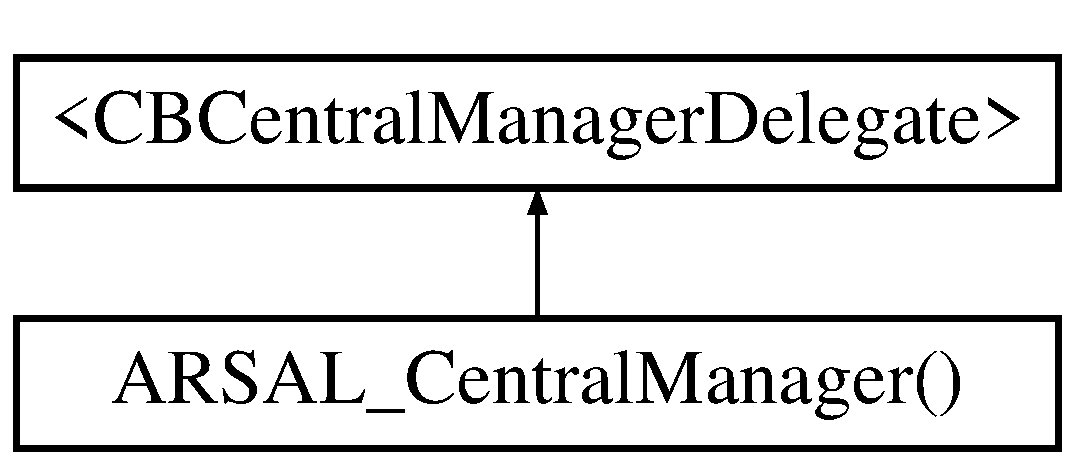
\includegraphics[height=2.000000cm]{categoryARSAL__CentralManager_07_08}
\end{center}
\end{figure}
\subsection*{Properties}
\begin{DoxyCompactItemize}
\item 
N\+S\+Mutable\+Array $\ast$ \hyperlink{categoryARSAL__CentralManager_07_08_a23828b5d378b496dd4f9950e15dee279}{delegate\+Array}
\item 
C\+B\+Central\+Manager $\ast$ \hyperlink{categoryARSAL__CentralManager_07_08_a7167856719a11298daa2ddcb610cc3b9}{central\+Manager}
\end{DoxyCompactItemize}


\subsection{Property Documentation}
\hypertarget{categoryARSAL__CentralManager_07_08_a7167856719a11298daa2ddcb610cc3b9}{}\label{categoryARSAL__CentralManager_07_08_a7167856719a11298daa2ddcb610cc3b9} 
\index{A\+R\+S\+A\+L\+\_\+\+Central\+Manager()@{A\+R\+S\+A\+L\+\_\+\+Central\+Manager()}!central\+Manager@{central\+Manager}}
\index{central\+Manager@{central\+Manager}!A\+R\+S\+A\+L\+\_\+\+Central\+Manager()@{A\+R\+S\+A\+L\+\_\+\+Central\+Manager()}}
\subsubsection{\texorpdfstring{central\+Manager}{centralManager}}
{\footnotesize\ttfamily -\/ (C\+B\+Central\+Manager$\ast$) central\+Manager\hspace{0.3cm}{\ttfamily [read]}, {\ttfamily [write]}, {\ttfamily [nonatomic]}, {\ttfamily [strong]}}

\hypertarget{categoryARSAL__CentralManager_07_08_a23828b5d378b496dd4f9950e15dee279}{}\label{categoryARSAL__CentralManager_07_08_a23828b5d378b496dd4f9950e15dee279} 
\index{A\+R\+S\+A\+L\+\_\+\+Central\+Manager()@{A\+R\+S\+A\+L\+\_\+\+Central\+Manager()}!delegate\+Array@{delegate\+Array}}
\index{delegate\+Array@{delegate\+Array}!A\+R\+S\+A\+L\+\_\+\+Central\+Manager()@{A\+R\+S\+A\+L\+\_\+\+Central\+Manager()}}
\subsubsection{\texorpdfstring{delegate\+Array}{delegateArray}}
{\footnotesize\ttfamily -\/ (N\+S\+Mutable\+Array$\ast$) delegate\+Array\hspace{0.3cm}{\ttfamily [read]}, {\ttfamily [write]}, {\ttfamily [nonatomic]}, {\ttfamily [strong]}}



The documentation for this category was generated from the following file\+:\begin{DoxyCompactItemize}
\item 
\hyperlink{ARSAL__CentralManager_8m}{A\+R\+S\+A\+L\+\_\+\+Central\+Manager.\+m}\end{DoxyCompactItemize}

\hypertarget{structARSAL__Sem__CustomImpl__t}{}\section{A\+R\+S\+A\+L\+\_\+\+Sem\+\_\+\+Custom\+Impl\+\_\+t Struct Reference}
\label{structARSAL__Sem__CustomImpl__t}\index{A\+R\+S\+A\+L\+\_\+\+Sem\+\_\+\+Custom\+Impl\+\_\+t@{A\+R\+S\+A\+L\+\_\+\+Sem\+\_\+\+Custom\+Impl\+\_\+t}}
\subsection*{Public Attributes}
\begin{DoxyCompactItemize}
\item 
A\+R\+S\+A\+L\+\_\+\+Mutex\+\_\+t \hyperlink{structARSAL__Sem__CustomImpl__t_a5b0c944edc475b603049210aa09f4383}{lock}
\item 
A\+R\+S\+A\+L\+\_\+\+Cond\+\_\+t \hyperlink{structARSAL__Sem__CustomImpl__t_ab67e2f2e89177d49e7ec68b55dc0a5c7}{cond}
\item 
int32\+\_\+t \hyperlink{structARSAL__Sem__CustomImpl__t_a14d1d2a87d385225e8b1bc61b87f5231}{count}
\end{DoxyCompactItemize}


\subsection{Member Data Documentation}
\hypertarget{structARSAL__Sem__CustomImpl__t_ab67e2f2e89177d49e7ec68b55dc0a5c7}{}\label{structARSAL__Sem__CustomImpl__t_ab67e2f2e89177d49e7ec68b55dc0a5c7} 
\index{A\+R\+S\+A\+L\+\_\+\+Sem\+\_\+\+Custom\+Impl\+\_\+t@{A\+R\+S\+A\+L\+\_\+\+Sem\+\_\+\+Custom\+Impl\+\_\+t}!cond@{cond}}
\index{cond@{cond}!A\+R\+S\+A\+L\+\_\+\+Sem\+\_\+\+Custom\+Impl\+\_\+t@{A\+R\+S\+A\+L\+\_\+\+Sem\+\_\+\+Custom\+Impl\+\_\+t}}
\subsubsection{\texorpdfstring{cond}{cond}}
{\footnotesize\ttfamily A\+R\+S\+A\+L\+\_\+\+Cond\+\_\+t A\+R\+S\+A\+L\+\_\+\+Sem\+\_\+\+Custom\+Impl\+\_\+t\+::cond}

\hypertarget{structARSAL__Sem__CustomImpl__t_a14d1d2a87d385225e8b1bc61b87f5231}{}\label{structARSAL__Sem__CustomImpl__t_a14d1d2a87d385225e8b1bc61b87f5231} 
\index{A\+R\+S\+A\+L\+\_\+\+Sem\+\_\+\+Custom\+Impl\+\_\+t@{A\+R\+S\+A\+L\+\_\+\+Sem\+\_\+\+Custom\+Impl\+\_\+t}!count@{count}}
\index{count@{count}!A\+R\+S\+A\+L\+\_\+\+Sem\+\_\+\+Custom\+Impl\+\_\+t@{A\+R\+S\+A\+L\+\_\+\+Sem\+\_\+\+Custom\+Impl\+\_\+t}}
\subsubsection{\texorpdfstring{count}{count}}
{\footnotesize\ttfamily int32\+\_\+t A\+R\+S\+A\+L\+\_\+\+Sem\+\_\+\+Custom\+Impl\+\_\+t\+::count}

\hypertarget{structARSAL__Sem__CustomImpl__t_a5b0c944edc475b603049210aa09f4383}{}\label{structARSAL__Sem__CustomImpl__t_a5b0c944edc475b603049210aa09f4383} 
\index{A\+R\+S\+A\+L\+\_\+\+Sem\+\_\+\+Custom\+Impl\+\_\+t@{A\+R\+S\+A\+L\+\_\+\+Sem\+\_\+\+Custom\+Impl\+\_\+t}!lock@{lock}}
\index{lock@{lock}!A\+R\+S\+A\+L\+\_\+\+Sem\+\_\+\+Custom\+Impl\+\_\+t@{A\+R\+S\+A\+L\+\_\+\+Sem\+\_\+\+Custom\+Impl\+\_\+t}}
\subsubsection{\texorpdfstring{lock}{lock}}
{\footnotesize\ttfamily A\+R\+S\+A\+L\+\_\+\+Mutex\+\_\+t A\+R\+S\+A\+L\+\_\+\+Sem\+\_\+\+Custom\+Impl\+\_\+t\+::lock}



The documentation for this struct was generated from the following file\+:\begin{DoxyCompactItemize}
\item 
\hyperlink{ARSAL__Sem_8c}{A\+R\+S\+A\+L\+\_\+\+Sem.\+c}\end{DoxyCompactItemize}

\hypertarget{classARSALBLEManagerNotification}{}\section{A\+R\+S\+A\+L\+B\+L\+E\+Manager\+Notification Class Reference}
\label{classARSALBLEManagerNotification}\index{A\+R\+S\+A\+L\+B\+L\+E\+Manager\+Notification@{A\+R\+S\+A\+L\+B\+L\+E\+Manager\+Notification}}


The documentation for this class was generated from the following file\+:\begin{DoxyCompactItemize}
\item 
\hyperlink{ARSAL__BLEManager_8m}{A\+R\+S\+A\+L\+\_\+\+B\+L\+E\+Manager.\+m}\end{DoxyCompactItemize}

\hypertarget{classARSALBLEManagerNotificationData}{}\section{A\+R\+S\+A\+L\+B\+L\+E\+Manager\+Notification\+Data Class Reference}
\label{classARSALBLEManagerNotificationData}\index{A\+R\+S\+A\+L\+B\+L\+E\+Manager\+Notification\+Data@{A\+R\+S\+A\+L\+B\+L\+E\+Manager\+Notification\+Data}}


The documentation for this class was generated from the following file\+:\begin{DoxyCompactItemize}
\item 
\hyperlink{ARSAL__BLEManager_8m}{A\+R\+S\+A\+L\+\_\+\+B\+L\+E\+Manager.\+m}\end{DoxyCompactItemize}

\hypertarget{categoryCBUUID_07StringExtraction_08}{}\section{C\+B\+U\+U\+ID(String\+Extraction) Category Reference}
\label{categoryCBUUID_07StringExtraction_08}\index{C\+B\+U\+U\+I\+D(\+String\+Extraction)@{C\+B\+U\+U\+I\+D(\+String\+Extraction)}}


{\ttfamily \#import $<$A\+R\+S\+A\+L\+\_\+\+B\+L\+E\+Manager.\+h$>$}

\subsection*{Instance Methods}
\begin{DoxyCompactItemize}
\item 
(N\+S\+String $\ast$) -\/ \hyperlink{categoryCBUUID_07StringExtraction_08_a5cba828d2015525ed0742841842f0418}{representative\+String}
\item 
(N\+S\+String $\ast$) -\/ \hyperlink{categoryCBUUID_07StringExtraction_08_a98d5f8fb2e5033d0024b604fd9bc8781}{short\+U\+U\+ID}
\end{DoxyCompactItemize}


\subsection{Method Documentation}
\hypertarget{categoryCBUUID_07StringExtraction_08_a5cba828d2015525ed0742841842f0418}{}\label{categoryCBUUID_07StringExtraction_08_a5cba828d2015525ed0742841842f0418} 
\index{C\+B\+U\+U\+I\+D(\+String\+Extraction)@{C\+B\+U\+U\+I\+D(\+String\+Extraction)}!representative\+String@{representative\+String}}
\index{representative\+String@{representative\+String}!C\+B\+U\+U\+I\+D(\+String\+Extraction)@{C\+B\+U\+U\+I\+D(\+String\+Extraction)}}
\subsubsection{\texorpdfstring{representative\+String()}{representativeString()}}
{\footnotesize\ttfamily -\/ (N\+S\+String $\ast$) representative\+String \begin{DoxyParamCaption}{ }\end{DoxyParamCaption}}

\hypertarget{categoryCBUUID_07StringExtraction_08_a98d5f8fb2e5033d0024b604fd9bc8781}{}\label{categoryCBUUID_07StringExtraction_08_a98d5f8fb2e5033d0024b604fd9bc8781} 
\index{C\+B\+U\+U\+I\+D(\+String\+Extraction)@{C\+B\+U\+U\+I\+D(\+String\+Extraction)}!short\+U\+U\+ID@{short\+U\+U\+ID}}
\index{short\+U\+U\+ID@{short\+U\+U\+ID}!C\+B\+U\+U\+I\+D(\+String\+Extraction)@{C\+B\+U\+U\+I\+D(\+String\+Extraction)}}
\subsubsection{\texorpdfstring{short\+U\+U\+I\+D()}{shortUUID()}}
{\footnotesize\ttfamily -\/ (N\+S\+String $\ast$) short\+U\+U\+ID \begin{DoxyParamCaption}{ }\end{DoxyParamCaption}}



The documentation for this category was generated from the following file\+:\begin{DoxyCompactItemize}
\item 
\hyperlink{ARSAL__BLEManager_8h}{A\+R\+S\+A\+L\+\_\+\+B\+L\+E\+Manager.\+h}\end{DoxyCompactItemize}

\hypertarget{structiovec}{}\section{iovec Struct Reference}
\label{structiovec}\index{iovec@{iovec}}
\subsection*{Public Attributes}
\begin{DoxyCompactItemize}
\item 
void $\ast$ \hyperlink{structiovec_a07aeddeccf80f14520fdd7ef0759442b}{iov\+\_\+base}
\item 
size\+\_\+t \hyperlink{structiovec_a17b5ac2078fd1adfabb262a95808a07d}{iov\+\_\+len}
\end{DoxyCompactItemize}


\subsection{Member Data Documentation}
\hypertarget{structiovec_a07aeddeccf80f14520fdd7ef0759442b}{}\label{structiovec_a07aeddeccf80f14520fdd7ef0759442b} 
\index{iovec@{iovec}!iov\+\_\+base@{iov\+\_\+base}}
\index{iov\+\_\+base@{iov\+\_\+base}!iovec@{iovec}}
\subsubsection{\texorpdfstring{iov\+\_\+base}{iov\_base}}
{\footnotesize\ttfamily void$\ast$ iovec\+::iov\+\_\+base}

\hypertarget{structiovec_a17b5ac2078fd1adfabb262a95808a07d}{}\label{structiovec_a17b5ac2078fd1adfabb262a95808a07d} 
\index{iovec@{iovec}!iov\+\_\+len@{iov\+\_\+len}}
\index{iov\+\_\+len@{iov\+\_\+len}!iovec@{iovec}}
\subsubsection{\texorpdfstring{iov\+\_\+len}{iov\_len}}
{\footnotesize\ttfamily size\+\_\+t iovec\+::iov\+\_\+len}



The documentation for this struct was generated from the following file\+:\begin{DoxyCompactItemize}
\item 
\hyperlink{ARSAL__Socket_8c}{A\+R\+S\+A\+L\+\_\+\+Socket.\+c}\end{DoxyCompactItemize}

\hypertarget{structMD5__CTX}{}\section{M\+D5\+\_\+\+C\+TX Struct Reference}
\label{structMD5__CTX}\index{M\+D5\+\_\+\+C\+TX@{M\+D5\+\_\+\+C\+TX}}


{\ttfamily \#include $<$md5.\+h$>$}

\subsection*{Public Attributes}
\begin{DoxyCompactItemize}
\item 
\hyperlink{md5_8h_ad854d8865ff7e0ce3717676b84926f54}{M\+D5\+\_\+u32plus} \hyperlink{structMD5__CTX_a90437ec62a8dda787f1667061d9755fe}{lo}
\item 
\hyperlink{md5_8h_ad854d8865ff7e0ce3717676b84926f54}{M\+D5\+\_\+u32plus} \hyperlink{structMD5__CTX_a3234f683810977ac629c2a8a05a1cc87}{hi}
\item 
\hyperlink{md5_8h_ad854d8865ff7e0ce3717676b84926f54}{M\+D5\+\_\+u32plus} \hyperlink{structMD5__CTX_abfbd731eb0b9d13a75ee4e49715e30b5}{a}
\item 
\hyperlink{md5_8h_ad854d8865ff7e0ce3717676b84926f54}{M\+D5\+\_\+u32plus} \hyperlink{structMD5__CTX_a63ef5819a909e0b4065796dfdac25962}{b}
\item 
\hyperlink{md5_8h_ad854d8865ff7e0ce3717676b84926f54}{M\+D5\+\_\+u32plus} \hyperlink{structMD5__CTX_a6226440d9b52200d32153df206fe3761}{c}
\item 
\hyperlink{md5_8h_ad854d8865ff7e0ce3717676b84926f54}{M\+D5\+\_\+u32plus} \hyperlink{structMD5__CTX_a3b2316dbfcad4bdb1306dc441761f396}{d}
\item 
unsigned char \hyperlink{structMD5__CTX_a2da73ecf544745f58211e998719f367f}{buffer} \mbox{[}64\mbox{]}
\item 
\hyperlink{md5_8h_ad854d8865ff7e0ce3717676b84926f54}{M\+D5\+\_\+u32plus} \hyperlink{structMD5__CTX_a2db62677a153981a205d225b051f0609}{block} \mbox{[}16\mbox{]}
\end{DoxyCompactItemize}


\subsection{Member Data Documentation}
\hypertarget{structMD5__CTX_abfbd731eb0b9d13a75ee4e49715e30b5}{}\label{structMD5__CTX_abfbd731eb0b9d13a75ee4e49715e30b5} 
\index{M\+D5\+\_\+\+C\+TX@{M\+D5\+\_\+\+C\+TX}!a@{a}}
\index{a@{a}!M\+D5\+\_\+\+C\+TX@{M\+D5\+\_\+\+C\+TX}}
\subsubsection{\texorpdfstring{a}{a}}
{\footnotesize\ttfamily \hyperlink{md5_8h_ad854d8865ff7e0ce3717676b84926f54}{M\+D5\+\_\+u32plus} M\+D5\+\_\+\+C\+T\+X\+::a}

\hypertarget{structMD5__CTX_a63ef5819a909e0b4065796dfdac25962}{}\label{structMD5__CTX_a63ef5819a909e0b4065796dfdac25962} 
\index{M\+D5\+\_\+\+C\+TX@{M\+D5\+\_\+\+C\+TX}!b@{b}}
\index{b@{b}!M\+D5\+\_\+\+C\+TX@{M\+D5\+\_\+\+C\+TX}}
\subsubsection{\texorpdfstring{b}{b}}
{\footnotesize\ttfamily \hyperlink{md5_8h_ad854d8865ff7e0ce3717676b84926f54}{M\+D5\+\_\+u32plus} M\+D5\+\_\+\+C\+T\+X\+::b}

\hypertarget{structMD5__CTX_a2db62677a153981a205d225b051f0609}{}\label{structMD5__CTX_a2db62677a153981a205d225b051f0609} 
\index{M\+D5\+\_\+\+C\+TX@{M\+D5\+\_\+\+C\+TX}!block@{block}}
\index{block@{block}!M\+D5\+\_\+\+C\+TX@{M\+D5\+\_\+\+C\+TX}}
\subsubsection{\texorpdfstring{block}{block}}
{\footnotesize\ttfamily \hyperlink{md5_8h_ad854d8865ff7e0ce3717676b84926f54}{M\+D5\+\_\+u32plus} M\+D5\+\_\+\+C\+T\+X\+::block\mbox{[}16\mbox{]}}

\hypertarget{structMD5__CTX_a2da73ecf544745f58211e998719f367f}{}\label{structMD5__CTX_a2da73ecf544745f58211e998719f367f} 
\index{M\+D5\+\_\+\+C\+TX@{M\+D5\+\_\+\+C\+TX}!buffer@{buffer}}
\index{buffer@{buffer}!M\+D5\+\_\+\+C\+TX@{M\+D5\+\_\+\+C\+TX}}
\subsubsection{\texorpdfstring{buffer}{buffer}}
{\footnotesize\ttfamily unsigned char M\+D5\+\_\+\+C\+T\+X\+::buffer\mbox{[}64\mbox{]}}

\hypertarget{structMD5__CTX_a6226440d9b52200d32153df206fe3761}{}\label{structMD5__CTX_a6226440d9b52200d32153df206fe3761} 
\index{M\+D5\+\_\+\+C\+TX@{M\+D5\+\_\+\+C\+TX}!c@{c}}
\index{c@{c}!M\+D5\+\_\+\+C\+TX@{M\+D5\+\_\+\+C\+TX}}
\subsubsection{\texorpdfstring{c}{c}}
{\footnotesize\ttfamily \hyperlink{md5_8h_ad854d8865ff7e0ce3717676b84926f54}{M\+D5\+\_\+u32plus} M\+D5\+\_\+\+C\+T\+X\+::c}

\hypertarget{structMD5__CTX_a3b2316dbfcad4bdb1306dc441761f396}{}\label{structMD5__CTX_a3b2316dbfcad4bdb1306dc441761f396} 
\index{M\+D5\+\_\+\+C\+TX@{M\+D5\+\_\+\+C\+TX}!d@{d}}
\index{d@{d}!M\+D5\+\_\+\+C\+TX@{M\+D5\+\_\+\+C\+TX}}
\subsubsection{\texorpdfstring{d}{d}}
{\footnotesize\ttfamily \hyperlink{md5_8h_ad854d8865ff7e0ce3717676b84926f54}{M\+D5\+\_\+u32plus} M\+D5\+\_\+\+C\+T\+X\+::d}

\hypertarget{structMD5__CTX_a3234f683810977ac629c2a8a05a1cc87}{}\label{structMD5__CTX_a3234f683810977ac629c2a8a05a1cc87} 
\index{M\+D5\+\_\+\+C\+TX@{M\+D5\+\_\+\+C\+TX}!hi@{hi}}
\index{hi@{hi}!M\+D5\+\_\+\+C\+TX@{M\+D5\+\_\+\+C\+TX}}
\subsubsection{\texorpdfstring{hi}{hi}}
{\footnotesize\ttfamily \hyperlink{md5_8h_ad854d8865ff7e0ce3717676b84926f54}{M\+D5\+\_\+u32plus} M\+D5\+\_\+\+C\+T\+X\+::hi}

\hypertarget{structMD5__CTX_a90437ec62a8dda787f1667061d9755fe}{}\label{structMD5__CTX_a90437ec62a8dda787f1667061d9755fe} 
\index{M\+D5\+\_\+\+C\+TX@{M\+D5\+\_\+\+C\+TX}!lo@{lo}}
\index{lo@{lo}!M\+D5\+\_\+\+C\+TX@{M\+D5\+\_\+\+C\+TX}}
\subsubsection{\texorpdfstring{lo}{lo}}
{\footnotesize\ttfamily \hyperlink{md5_8h_ad854d8865ff7e0ce3717676b84926f54}{M\+D5\+\_\+u32plus} M\+D5\+\_\+\+C\+T\+X\+::lo}



The documentation for this struct was generated from the following file\+:\begin{DoxyCompactItemize}
\item 
\hyperlink{md5_8h}{md5.\+h}\end{DoxyCompactItemize}

\chapter{File Documentation}
\hypertarget{ARSAL__BLEManager_8m}{}\section{A\+R\+S\+A\+L\+\_\+\+B\+L\+E\+Manager.\+m File Reference}
\label{ARSAL__BLEManager_8m}\index{A\+R\+S\+A\+L\+\_\+\+B\+L\+E\+Manager.\+m@{A\+R\+S\+A\+L\+\_\+\+B\+L\+E\+Manager.\+m}}


B\+LE network manager allow to send over ble network.  


{\ttfamily \#include \char`\"{}lib\+A\+R\+S\+A\+L/\+A\+R\+S\+A\+L\+\_\+\+B\+L\+E\+Manager.\+h\char`\"{}}\newline
{\ttfamily \#include \char`\"{}lib\+A\+R\+S\+A\+L/\+A\+R\+S\+A\+L\+\_\+\+Error.\+h\char`\"{}}\newline
\subsection*{Macros}
\begin{DoxyCompactItemize}
\item 
\#define \hyperlink{ARSAL__BLEManager_8m_a677994a12e7905d8e94de1a85fba9ef2}{A\+R\+S\+A\+L\+\_\+\+B\+L\+E\+M\+A\+N\+A\+G\+E\+R\+\_\+\+E\+N\+A\+B\+L\+E\+\_\+\+D\+E\+B\+UG}~(0)
\item 
\#define \hyperlink{ARSAL__BLEManager_8m_a90d93883db518a02ed00842a3beb7ae1}{A\+R\+S\+A\+L\+\_\+\+B\+L\+E\+M\+A\+N\+A\+G\+E\+R\+\_\+\+C\+O\+N\+N\+E\+C\+T\+I\+O\+N\+\_\+\+T\+I\+M\+E\+O\+U\+T\+\_\+\+S\+EC}~(5)
\end{DoxyCompactItemize}


\subsection{Detailed Description}
B\+LE network manager allow to send over ble network. 

wifi network manager allow to send over wifi network. \begin{DoxyDate}{Date}
06/11/2013 
\end{DoxyDate}
\begin{DoxyAuthor}{Author}
\href{mailto:frederic.dhaeyer@parrot.com}{\tt frederic.\+dhaeyer@parrot.\+com} 
\end{DoxyAuthor}


\subsection{Macro Definition Documentation}
\hypertarget{ARSAL__BLEManager_8m_a90d93883db518a02ed00842a3beb7ae1}{}\label{ARSAL__BLEManager_8m_a90d93883db518a02ed00842a3beb7ae1} 
\index{A\+R\+S\+A\+L\+\_\+\+B\+L\+E\+Manager.\+m@{A\+R\+S\+A\+L\+\_\+\+B\+L\+E\+Manager.\+m}!A\+R\+S\+A\+L\+\_\+\+B\+L\+E\+M\+A\+N\+A\+G\+E\+R\+\_\+\+C\+O\+N\+N\+E\+C\+T\+I\+O\+N\+\_\+\+T\+I\+M\+E\+O\+U\+T\+\_\+\+S\+EC@{A\+R\+S\+A\+L\+\_\+\+B\+L\+E\+M\+A\+N\+A\+G\+E\+R\+\_\+\+C\+O\+N\+N\+E\+C\+T\+I\+O\+N\+\_\+\+T\+I\+M\+E\+O\+U\+T\+\_\+\+S\+EC}}
\index{A\+R\+S\+A\+L\+\_\+\+B\+L\+E\+M\+A\+N\+A\+G\+E\+R\+\_\+\+C\+O\+N\+N\+E\+C\+T\+I\+O\+N\+\_\+\+T\+I\+M\+E\+O\+U\+T\+\_\+\+S\+EC@{A\+R\+S\+A\+L\+\_\+\+B\+L\+E\+M\+A\+N\+A\+G\+E\+R\+\_\+\+C\+O\+N\+N\+E\+C\+T\+I\+O\+N\+\_\+\+T\+I\+M\+E\+O\+U\+T\+\_\+\+S\+EC}!A\+R\+S\+A\+L\+\_\+\+B\+L\+E\+Manager.\+m@{A\+R\+S\+A\+L\+\_\+\+B\+L\+E\+Manager.\+m}}
\subsubsection{\texorpdfstring{A\+R\+S\+A\+L\+\_\+\+B\+L\+E\+M\+A\+N\+A\+G\+E\+R\+\_\+\+C\+O\+N\+N\+E\+C\+T\+I\+O\+N\+\_\+\+T\+I\+M\+E\+O\+U\+T\+\_\+\+S\+EC}{ARSAL\_BLEMANAGER\_CONNECTION\_TIMEOUT\_SEC}}
{\footnotesize\ttfamily \#define A\+R\+S\+A\+L\+\_\+\+B\+L\+E\+M\+A\+N\+A\+G\+E\+R\+\_\+\+C\+O\+N\+N\+E\+C\+T\+I\+O\+N\+\_\+\+T\+I\+M\+E\+O\+U\+T\+\_\+\+S\+EC~(5)}

\hypertarget{ARSAL__BLEManager_8m_a677994a12e7905d8e94de1a85fba9ef2}{}\label{ARSAL__BLEManager_8m_a677994a12e7905d8e94de1a85fba9ef2} 
\index{A\+R\+S\+A\+L\+\_\+\+B\+L\+E\+Manager.\+m@{A\+R\+S\+A\+L\+\_\+\+B\+L\+E\+Manager.\+m}!A\+R\+S\+A\+L\+\_\+\+B\+L\+E\+M\+A\+N\+A\+G\+E\+R\+\_\+\+E\+N\+A\+B\+L\+E\+\_\+\+D\+E\+B\+UG@{A\+R\+S\+A\+L\+\_\+\+B\+L\+E\+M\+A\+N\+A\+G\+E\+R\+\_\+\+E\+N\+A\+B\+L\+E\+\_\+\+D\+E\+B\+UG}}
\index{A\+R\+S\+A\+L\+\_\+\+B\+L\+E\+M\+A\+N\+A\+G\+E\+R\+\_\+\+E\+N\+A\+B\+L\+E\+\_\+\+D\+E\+B\+UG@{A\+R\+S\+A\+L\+\_\+\+B\+L\+E\+M\+A\+N\+A\+G\+E\+R\+\_\+\+E\+N\+A\+B\+L\+E\+\_\+\+D\+E\+B\+UG}!A\+R\+S\+A\+L\+\_\+\+B\+L\+E\+Manager.\+m@{A\+R\+S\+A\+L\+\_\+\+B\+L\+E\+Manager.\+m}}
\subsubsection{\texorpdfstring{A\+R\+S\+A\+L\+\_\+\+B\+L\+E\+M\+A\+N\+A\+G\+E\+R\+\_\+\+E\+N\+A\+B\+L\+E\+\_\+\+D\+E\+B\+UG}{ARSAL\_BLEMANAGER\_ENABLE\_DEBUG}}
{\footnotesize\ttfamily \#define A\+R\+S\+A\+L\+\_\+\+B\+L\+E\+M\+A\+N\+A\+G\+E\+R\+\_\+\+E\+N\+A\+B\+L\+E\+\_\+\+D\+E\+B\+UG~(0)}


\hypertarget{ARSAL__CentralManager_8m}{}\section{A\+R\+S\+A\+L\+\_\+\+Central\+Manager.\+m File Reference}
\label{ARSAL__CentralManager_8m}\index{A\+R\+S\+A\+L\+\_\+\+Central\+Manager.\+m@{A\+R\+S\+A\+L\+\_\+\+Central\+Manager.\+m}}
{\ttfamily \#import \char`\"{}lib\+A\+R\+S\+A\+L/\+A\+R\+S\+A\+L\+\_\+\+Central\+Manager.\+h\char`\"{}}\newline

\hypertarget{ARSAL__Ftw_8c}{}\section{A\+R\+S\+A\+L\+\_\+\+Ftw.\+c File Reference}
\label{ARSAL__Ftw_8c}\index{A\+R\+S\+A\+L\+\_\+\+Ftw.\+c@{A\+R\+S\+A\+L\+\_\+\+Ftw.\+c}}


lib\+A\+R\+S\+AL Ftw file provides ftw/nftw abstraction U\+N\+IX i\+OS, or implementation for Android.  


{\ttfamily \#include $<$config.\+h$>$}\newline
{\ttfamily \#include $<$sys/types.\+h$>$}\newline
{\ttfamily \#include $<$stdlib.\+h$>$}\newline
{\ttfamily \#include $<$sys/stat.\+h$>$}\newline
{\ttfamily \#include \char`\"{}lib\+A\+R\+S\+A\+L/\+A\+R\+S\+A\+L\+\_\+\+Ftw.\+h\char`\"{}}\newline
{\ttfamily \#include \char`\"{}lib\+A\+R\+S\+A\+L/\+A\+R\+S\+A\+L\+\_\+\+Print.\+h\char`\"{}}\newline
{\ttfamily \#include $<$dirent.\+h$>$}\newline
{\ttfamily \#include \char`\"{}A\+R\+S\+A\+L\+\_\+\+Ftw.\+h\char`\"{}}\newline
\subsection*{Macros}
\begin{DoxyCompactItemize}
\item 
\#define \hyperlink{ARSAL__Ftw_8c_a440cfe6a995a624f61aaa9dc6cccf8f1}{A\+R\+S\+A\+L\+\_\+\+F\+T\+W\+\_\+\+T\+AG}~\char`\"{}Ftw\char`\"{}
\end{DoxyCompactItemize}
\subsection*{Functions}
\begin{DoxyCompactItemize}
\item 
int \hyperlink{ARSAL__Ftw_8c_acb76ab9a45a78e45960d60c3112f8771}{A\+R\+S\+A\+L\+\_\+\+Ftw} (const char $\ast$dirpath, A\+R\+S\+A\+L\+\_\+\+Ftw\+Callback cb, int nopenfd)
\item 
int \hyperlink{ARSAL__Ftw_8c_ac655e97ab59baa526ce37336fa5d47c7}{A\+R\+S\+A\+L\+\_\+\+Nftw} (const char $\ast$dirpath, A\+R\+S\+A\+L\+\_\+\+Nftw\+Callback cb, int nopenfd, e\+A\+R\+S\+A\+L\+\_\+\+F\+T\+W\+\_\+\+F\+L\+AG flags)
\item 
int \hyperlink{ARSAL__Ftw_8c_a912a8e5f1e0943dbcbd0409f085f23d8}{A\+R\+S\+A\+L\+\_\+\+Ftw\+\_\+internal} (const char $\ast$dir\+Path, A\+R\+S\+A\+L\+\_\+\+Ftw\+Callback cb, int nopenfd)
\begin{DoxyCompactList}\small\item\em ftw-\/like function legacy support implementation, Recursively descends the directory hierarchy \end{DoxyCompactList}\item 
int \hyperlink{ARSAL__Ftw_8c_a63f832f62c5d379678db44ab81b601c3}{A\+R\+S\+A\+L\+\_\+\+Nftw\+\_\+internal} (const char $\ast$dir\+Path, A\+R\+S\+A\+L\+\_\+\+Nftw\+Callback cb, int nopenfd, e\+A\+R\+S\+A\+L\+\_\+\+F\+T\+W\+\_\+\+F\+L\+AG flags, int current\+Level, int current\+Base)
\begin{DoxyCompactList}\small\item\em nftw-\/like function legacy support implementation, recursively descends the directory hierarchy \end{DoxyCompactList}\end{DoxyCompactItemize}


\subsection{Detailed Description}
lib\+A\+R\+S\+AL Ftw file provides ftw/nftw abstraction U\+N\+IX i\+OS, or implementation for Android. 

\begin{DoxyDate}{Date}
19/12/2013 
\end{DoxyDate}
\begin{DoxyAuthor}{Author}
\href{mailto:david.flattin.ext@parrot.com}{\tt david.\+flattin.\+ext@parrot.\+com} 
\end{DoxyAuthor}


\subsection{Macro Definition Documentation}
\hypertarget{ARSAL__Ftw_8c_a440cfe6a995a624f61aaa9dc6cccf8f1}{}\label{ARSAL__Ftw_8c_a440cfe6a995a624f61aaa9dc6cccf8f1} 
\index{A\+R\+S\+A\+L\+\_\+\+Ftw.\+c@{A\+R\+S\+A\+L\+\_\+\+Ftw.\+c}!A\+R\+S\+A\+L\+\_\+\+F\+T\+W\+\_\+\+T\+AG@{A\+R\+S\+A\+L\+\_\+\+F\+T\+W\+\_\+\+T\+AG}}
\index{A\+R\+S\+A\+L\+\_\+\+F\+T\+W\+\_\+\+T\+AG@{A\+R\+S\+A\+L\+\_\+\+F\+T\+W\+\_\+\+T\+AG}!A\+R\+S\+A\+L\+\_\+\+Ftw.\+c@{A\+R\+S\+A\+L\+\_\+\+Ftw.\+c}}
\subsubsection{\texorpdfstring{A\+R\+S\+A\+L\+\_\+\+F\+T\+W\+\_\+\+T\+AG}{ARSAL\_FTW\_TAG}}
{\footnotesize\ttfamily \#define A\+R\+S\+A\+L\+\_\+\+F\+T\+W\+\_\+\+T\+AG~\char`\"{}Ftw\char`\"{}}



\subsection{Function Documentation}
\hypertarget{ARSAL__Ftw_8c_acb76ab9a45a78e45960d60c3112f8771}{}\label{ARSAL__Ftw_8c_acb76ab9a45a78e45960d60c3112f8771} 
\index{A\+R\+S\+A\+L\+\_\+\+Ftw.\+c@{A\+R\+S\+A\+L\+\_\+\+Ftw.\+c}!A\+R\+S\+A\+L\+\_\+\+Ftw@{A\+R\+S\+A\+L\+\_\+\+Ftw}}
\index{A\+R\+S\+A\+L\+\_\+\+Ftw@{A\+R\+S\+A\+L\+\_\+\+Ftw}!A\+R\+S\+A\+L\+\_\+\+Ftw.\+c@{A\+R\+S\+A\+L\+\_\+\+Ftw.\+c}}
\subsubsection{\texorpdfstring{A\+R\+S\+A\+L\+\_\+\+Ftw()}{ARSAL\_Ftw()}}
{\footnotesize\ttfamily int A\+R\+S\+A\+L\+\_\+\+Ftw (\begin{DoxyParamCaption}\item[{const char $\ast$}]{dirpath,  }\item[{A\+R\+S\+A\+L\+\_\+\+Ftw\+Callback}]{cb,  }\item[{int}]{nopenfd }\end{DoxyParamCaption})}

\hypertarget{ARSAL__Ftw_8c_a912a8e5f1e0943dbcbd0409f085f23d8}{}\label{ARSAL__Ftw_8c_a912a8e5f1e0943dbcbd0409f085f23d8} 
\index{A\+R\+S\+A\+L\+\_\+\+Ftw.\+c@{A\+R\+S\+A\+L\+\_\+\+Ftw.\+c}!A\+R\+S\+A\+L\+\_\+\+Ftw\+\_\+internal@{A\+R\+S\+A\+L\+\_\+\+Ftw\+\_\+internal}}
\index{A\+R\+S\+A\+L\+\_\+\+Ftw\+\_\+internal@{A\+R\+S\+A\+L\+\_\+\+Ftw\+\_\+internal}!A\+R\+S\+A\+L\+\_\+\+Ftw.\+c@{A\+R\+S\+A\+L\+\_\+\+Ftw.\+c}}
\subsubsection{\texorpdfstring{A\+R\+S\+A\+L\+\_\+\+Ftw\+\_\+internal()}{ARSAL\_Ftw\_internal()}}
{\footnotesize\ttfamily int A\+R\+S\+A\+L\+\_\+\+Ftw\+\_\+internal (\begin{DoxyParamCaption}\item[{const char $\ast$}]{dir\+Path,  }\item[{A\+R\+S\+A\+L\+\_\+\+Ftw\+Callback}]{cb,  }\item[{int}]{nopenfd }\end{DoxyParamCaption})}



ftw-\/like function legacy support implementation, Recursively descends the directory hierarchy 

fwt-\/like function \hypertarget{ARSAL__Ftw_8c_ac655e97ab59baa526ce37336fa5d47c7}{}\label{ARSAL__Ftw_8c_ac655e97ab59baa526ce37336fa5d47c7} 
\index{A\+R\+S\+A\+L\+\_\+\+Ftw.\+c@{A\+R\+S\+A\+L\+\_\+\+Ftw.\+c}!A\+R\+S\+A\+L\+\_\+\+Nftw@{A\+R\+S\+A\+L\+\_\+\+Nftw}}
\index{A\+R\+S\+A\+L\+\_\+\+Nftw@{A\+R\+S\+A\+L\+\_\+\+Nftw}!A\+R\+S\+A\+L\+\_\+\+Ftw.\+c@{A\+R\+S\+A\+L\+\_\+\+Ftw.\+c}}
\subsubsection{\texorpdfstring{A\+R\+S\+A\+L\+\_\+\+Nftw()}{ARSAL\_Nftw()}}
{\footnotesize\ttfamily int A\+R\+S\+A\+L\+\_\+\+Nftw (\begin{DoxyParamCaption}\item[{const char $\ast$}]{dirpath,  }\item[{A\+R\+S\+A\+L\+\_\+\+Nftw\+Callback}]{cb,  }\item[{int}]{nopenfd,  }\item[{e\+A\+R\+S\+A\+L\+\_\+\+F\+T\+W\+\_\+\+F\+L\+AG}]{flags }\end{DoxyParamCaption})}

\hypertarget{ARSAL__Ftw_8c_a63f832f62c5d379678db44ab81b601c3}{}\label{ARSAL__Ftw_8c_a63f832f62c5d379678db44ab81b601c3} 
\index{A\+R\+S\+A\+L\+\_\+\+Ftw.\+c@{A\+R\+S\+A\+L\+\_\+\+Ftw.\+c}!A\+R\+S\+A\+L\+\_\+\+Nftw\+\_\+internal@{A\+R\+S\+A\+L\+\_\+\+Nftw\+\_\+internal}}
\index{A\+R\+S\+A\+L\+\_\+\+Nftw\+\_\+internal@{A\+R\+S\+A\+L\+\_\+\+Nftw\+\_\+internal}!A\+R\+S\+A\+L\+\_\+\+Ftw.\+c@{A\+R\+S\+A\+L\+\_\+\+Ftw.\+c}}
\subsubsection{\texorpdfstring{A\+R\+S\+A\+L\+\_\+\+Nftw\+\_\+internal()}{ARSAL\_Nftw\_internal()}}
{\footnotesize\ttfamily int A\+R\+S\+A\+L\+\_\+\+Nftw\+\_\+internal (\begin{DoxyParamCaption}\item[{const char $\ast$}]{dir\+Path,  }\item[{A\+R\+S\+A\+L\+\_\+\+Nftw\+Callback}]{cb,  }\item[{int}]{nopenfd,  }\item[{e\+A\+R\+S\+A\+L\+\_\+\+F\+T\+W\+\_\+\+F\+L\+AG}]{flags,  }\item[{int}]{current\+Level,  }\item[{int}]{current\+Base }\end{DoxyParamCaption})}



nftw-\/like function legacy support implementation, recursively descends the directory hierarchy 

nftw-\/like function 
\hypertarget{ARSAL__Ftw_8h}{}\section{A\+R\+S\+A\+L\+\_\+\+Ftw.\+h File Reference}
\label{ARSAL__Ftw_8h}\index{A\+R\+S\+A\+L\+\_\+\+Ftw.\+h@{A\+R\+S\+A\+L\+\_\+\+Ftw.\+h}}


lib\+A\+R\+S\+AL Ftw header file.  


\subsection*{Enumerations}
\begin{DoxyCompactItemize}
\item 
enum \hyperlink{ARSAL__Ftw_8h_a0b7606fe246b0ca2fa31ae93ba796f34}{e\+A\+R\+S\+A\+L\+\_\+\+F\+T\+W\+\_\+\+R\+E\+S\+U\+LT} \{ \hyperlink{ARSAL__Ftw_8h_a0b7606fe246b0ca2fa31ae93ba796f34a26ecc27b14bdc0a312d718dee6833680}{A\+R\+S\+A\+L\+\_\+\+F\+T\+W\+\_\+\+F\+A\+IL} = 0, 
\hyperlink{ARSAL__Ftw_8h_a0b7606fe246b0ca2fa31ae93ba796f34ac462bf82940791a2783cf6af36104229}{A\+R\+S\+A\+L\+\_\+\+F\+T\+W\+\_\+\+OK}
 \}
\end{DoxyCompactItemize}
\subsection*{Functions}
\begin{DoxyCompactItemize}
\item 
int \hyperlink{ARSAL__Ftw_8h_a912a8e5f1e0943dbcbd0409f085f23d8}{A\+R\+S\+A\+L\+\_\+\+Ftw\+\_\+internal} (const char $\ast$dir\+Path, A\+R\+S\+A\+L\+\_\+\+Ftw\+Callback cb, int nopenfd)
\begin{DoxyCompactList}\small\item\em ftw-\/like function legacy support implementation, Recursively descends the directory hierarchy \end{DoxyCompactList}\item 
int \hyperlink{ARSAL__Ftw_8h_a63f832f62c5d379678db44ab81b601c3}{A\+R\+S\+A\+L\+\_\+\+Nftw\+\_\+internal} (const char $\ast$dir\+Path, A\+R\+S\+A\+L\+\_\+\+Nftw\+Callback cb, int nopenfd, e\+A\+R\+S\+A\+L\+\_\+\+F\+T\+W\+\_\+\+F\+L\+AG flags, int current\+Level, int current\+Base)
\begin{DoxyCompactList}\small\item\em nftw-\/like function legacy support implementation, recursively descends the directory hierarchy \end{DoxyCompactList}\end{DoxyCompactItemize}


\subsection{Detailed Description}
lib\+A\+R\+S\+AL Ftw header file. 

\begin{DoxyDate}{Date}
19/12/2013 
\end{DoxyDate}
\begin{DoxyAuthor}{Author}
\href{mailto:david.flattin.ext@parrot.com}{\tt david.\+flattin.\+ext@parrot.\+com} 
\end{DoxyAuthor}


\subsection{Enumeration Type Documentation}
\hypertarget{ARSAL__Ftw_8h_a0b7606fe246b0ca2fa31ae93ba796f34}{}\label{ARSAL__Ftw_8h_a0b7606fe246b0ca2fa31ae93ba796f34} 
\index{A\+R\+S\+A\+L\+\_\+\+Ftw.\+h@{A\+R\+S\+A\+L\+\_\+\+Ftw.\+h}!e\+A\+R\+S\+A\+L\+\_\+\+F\+T\+W\+\_\+\+R\+E\+S\+U\+LT@{e\+A\+R\+S\+A\+L\+\_\+\+F\+T\+W\+\_\+\+R\+E\+S\+U\+LT}}
\index{e\+A\+R\+S\+A\+L\+\_\+\+F\+T\+W\+\_\+\+R\+E\+S\+U\+LT@{e\+A\+R\+S\+A\+L\+\_\+\+F\+T\+W\+\_\+\+R\+E\+S\+U\+LT}!A\+R\+S\+A\+L\+\_\+\+Ftw.\+h@{A\+R\+S\+A\+L\+\_\+\+Ftw.\+h}}
\subsubsection{\texorpdfstring{e\+A\+R\+S\+A\+L\+\_\+\+F\+T\+W\+\_\+\+R\+E\+S\+U\+LT}{eARSAL\_FTW\_RESULT}}
{\footnotesize\ttfamily enum \hyperlink{ARSAL__Ftw_8h_a0b7606fe246b0ca2fa31ae93ba796f34}{e\+A\+R\+S\+A\+L\+\_\+\+F\+T\+W\+\_\+\+R\+E\+S\+U\+LT}}

Custom incomplete ftw/nftw implementation for system without support (Android as of ndk r7, r8, r9) Internal result values get from A\+R\+S\+A\+L\+\_\+\+Nftw\+Callback return analyse \begin{DoxyEnumFields}{Enumerator}
\raisebox{\heightof{T}}[0pt][0pt]{\index{A\+R\+S\+A\+L\+\_\+\+F\+T\+W\+\_\+\+F\+A\+IL@{A\+R\+S\+A\+L\+\_\+\+F\+T\+W\+\_\+\+F\+A\+IL}!A\+R\+S\+A\+L\+\_\+\+Ftw.\+h@{A\+R\+S\+A\+L\+\_\+\+Ftw.\+h}}\index{A\+R\+S\+A\+L\+\_\+\+Ftw.\+h@{A\+R\+S\+A\+L\+\_\+\+Ftw.\+h}!A\+R\+S\+A\+L\+\_\+\+F\+T\+W\+\_\+\+F\+A\+IL@{A\+R\+S\+A\+L\+\_\+\+F\+T\+W\+\_\+\+F\+A\+IL}}}\hypertarget{ARSAL__Ftw_8h_a0b7606fe246b0ca2fa31ae93ba796f34a26ecc27b14bdc0a312d718dee6833680}{}\label{ARSAL__Ftw_8h_a0b7606fe246b0ca2fa31ae93ba796f34a26ecc27b14bdc0a312d718dee6833680} 
A\+R\+S\+A\+L\+\_\+\+F\+T\+W\+\_\+\+F\+A\+IL&\\
\hline

\raisebox{\heightof{T}}[0pt][0pt]{\index{A\+R\+S\+A\+L\+\_\+\+F\+T\+W\+\_\+\+OK@{A\+R\+S\+A\+L\+\_\+\+F\+T\+W\+\_\+\+OK}!A\+R\+S\+A\+L\+\_\+\+Ftw.\+h@{A\+R\+S\+A\+L\+\_\+\+Ftw.\+h}}\index{A\+R\+S\+A\+L\+\_\+\+Ftw.\+h@{A\+R\+S\+A\+L\+\_\+\+Ftw.\+h}!A\+R\+S\+A\+L\+\_\+\+F\+T\+W\+\_\+\+OK@{A\+R\+S\+A\+L\+\_\+\+F\+T\+W\+\_\+\+OK}}}\hypertarget{ARSAL__Ftw_8h_a0b7606fe246b0ca2fa31ae93ba796f34ac462bf82940791a2783cf6af36104229}{}\label{ARSAL__Ftw_8h_a0b7606fe246b0ca2fa31ae93ba796f34ac462bf82940791a2783cf6af36104229} 
A\+R\+S\+A\+L\+\_\+\+F\+T\+W\+\_\+\+OK&\\
\hline

\end{DoxyEnumFields}


\subsection{Function Documentation}
\hypertarget{ARSAL__Ftw_8h_a912a8e5f1e0943dbcbd0409f085f23d8}{}\label{ARSAL__Ftw_8h_a912a8e5f1e0943dbcbd0409f085f23d8} 
\index{A\+R\+S\+A\+L\+\_\+\+Ftw.\+h@{A\+R\+S\+A\+L\+\_\+\+Ftw.\+h}!A\+R\+S\+A\+L\+\_\+\+Ftw\+\_\+internal@{A\+R\+S\+A\+L\+\_\+\+Ftw\+\_\+internal}}
\index{A\+R\+S\+A\+L\+\_\+\+Ftw\+\_\+internal@{A\+R\+S\+A\+L\+\_\+\+Ftw\+\_\+internal}!A\+R\+S\+A\+L\+\_\+\+Ftw.\+h@{A\+R\+S\+A\+L\+\_\+\+Ftw.\+h}}
\subsubsection{\texorpdfstring{A\+R\+S\+A\+L\+\_\+\+Ftw\+\_\+internal()}{ARSAL\_Ftw\_internal()}}
{\footnotesize\ttfamily int A\+R\+S\+A\+L\+\_\+\+Ftw\+\_\+internal (\begin{DoxyParamCaption}\item[{const char $\ast$}]{dir\+Path,  }\item[{A\+R\+S\+A\+L\+\_\+\+Ftw\+Callback}]{cb,  }\item[{int}]{nopenfd }\end{DoxyParamCaption})}



ftw-\/like function legacy support implementation, Recursively descends the directory hierarchy 


\begin{DoxyParams}{Parameters}
{\em dirpath} & The directory to descend \\
\hline
{\em cb} & The callback recursively on each element of run through the directories \\
\hline
{\em nopenfd} & The maximum number of directories depth \\
\hline
\end{DoxyParams}

\begin{DoxyRetVals}{Return values}
{\em On} & success, returns 0. Otherwise, it returns -\/1, or callack user value \\
\hline
\end{DoxyRetVals}
\begin{DoxySeeAlso}{See also}
ftw standard documentation
\end{DoxySeeAlso}
fwt-\/like function \hypertarget{ARSAL__Ftw_8h_a63f832f62c5d379678db44ab81b601c3}{}\label{ARSAL__Ftw_8h_a63f832f62c5d379678db44ab81b601c3} 
\index{A\+R\+S\+A\+L\+\_\+\+Ftw.\+h@{A\+R\+S\+A\+L\+\_\+\+Ftw.\+h}!A\+R\+S\+A\+L\+\_\+\+Nftw\+\_\+internal@{A\+R\+S\+A\+L\+\_\+\+Nftw\+\_\+internal}}
\index{A\+R\+S\+A\+L\+\_\+\+Nftw\+\_\+internal@{A\+R\+S\+A\+L\+\_\+\+Nftw\+\_\+internal}!A\+R\+S\+A\+L\+\_\+\+Ftw.\+h@{A\+R\+S\+A\+L\+\_\+\+Ftw.\+h}}
\subsubsection{\texorpdfstring{A\+R\+S\+A\+L\+\_\+\+Nftw\+\_\+internal()}{ARSAL\_Nftw\_internal()}}
{\footnotesize\ttfamily int A\+R\+S\+A\+L\+\_\+\+Nftw\+\_\+internal (\begin{DoxyParamCaption}\item[{const char $\ast$}]{dir\+Path,  }\item[{A\+R\+S\+A\+L\+\_\+\+Nftw\+Callback}]{cb,  }\item[{int}]{nopenfd,  }\item[{e\+A\+R\+S\+A\+L\+\_\+\+F\+T\+W\+\_\+\+F\+L\+AG}]{flags,  }\item[{int}]{current\+Level,  }\item[{int}]{current\+Base }\end{DoxyParamCaption})}



nftw-\/like function legacy support implementation, recursively descends the directory hierarchy 


\begin{DoxyParams}{Parameters}
{\em dirpath} & The directory to descend \\
\hline
{\em cb} & The callback recursively on each element of run through the directories \\
\hline
{\em nopenfd} & The maximum number of directories depth \\
\hline
{\em flags} & The flag of the type of tree explore \\
\hline
{\em current\+Level} & The current depth level, should be 0 \\
\hline
{\em current\+Base} & The base depth level, should be 0 \\
\hline
\end{DoxyParams}

\begin{DoxyRetVals}{Return values}
{\em On} & success, returns 0. Otherwise, it returns -\/1, or callack user value \\
\hline
\end{DoxyRetVals}
\begin{DoxySeeAlso}{See also}
nftw standard documentation
\end{DoxySeeAlso}
nftw-\/like function 
\hypertarget{ARSAL__MD5_8c}{}\section{A\+R\+S\+A\+L\+\_\+\+M\+D5.\+c File Reference}
\label{ARSAL__MD5_8c}\index{A\+R\+S\+A\+L\+\_\+\+M\+D5.\+c@{A\+R\+S\+A\+L\+\_\+\+M\+D5.\+c}}


M\+D5 manager allow compute and check md5.  


{\ttfamily \#include $<$stdio.\+h$>$}\newline
{\ttfamily \#include \char`\"{}md5.\+h\char`\"{}}\newline
{\ttfamily \#include \char`\"{}lib\+A\+R\+S\+A\+L/\+A\+R\+S\+A\+L\+\_\+\+Error.\+h\char`\"{}}\newline
{\ttfamily \#include \char`\"{}lib\+A\+R\+S\+A\+L/\+A\+R\+S\+A\+L\+\_\+\+Print.\+h\char`\"{}}\newline
{\ttfamily \#include \char`\"{}lib\+A\+R\+S\+A\+L/\+A\+R\+S\+A\+L\+\_\+\+M\+D5\+\_\+\+Manager.\+h\char`\"{}}\newline
{\ttfamily \#include \char`\"{}A\+R\+S\+A\+L\+\_\+\+M\+D5.\+h\char`\"{}}\newline
\subsection*{Macros}
\begin{DoxyCompactItemize}
\item 
\#define \hyperlink{ARSAL__MD5_8c_a1f6c511e70ee202b0c50b5590053cd9c}{A\+R\+U\+T\+I\+L\+S\+\_\+\+M\+D5\+\_\+\+T\+AG}~\char`\"{}Md5\char`\"{}
\end{DoxyCompactItemize}
\subsection*{Functions}
\begin{DoxyCompactItemize}
\item 
e\+A\+R\+S\+A\+L\+\_\+\+E\+R\+R\+OR \hyperlink{ARSAL__MD5_8c_ad1dfea64c506a9687561d4086e78570a}{A\+R\+S\+A\+L\+\_\+\+M\+D5\+\_\+\+Manager\+\_\+\+Init} (A\+R\+S\+A\+L\+\_\+\+M\+D5\+\_\+\+Manager\+\_\+t $\ast$manager)
\item 
void \hyperlink{ARSAL__MD5_8c_a8f4ef6da24327f4032e7d24c934dfc8d}{A\+R\+S\+A\+L\+\_\+\+M\+D5\+\_\+\+Manager\+\_\+\+Close} (A\+R\+S\+A\+L\+\_\+\+M\+D5\+\_\+\+Manager\+\_\+t $\ast$manager)
\item 
e\+A\+R\+S\+A\+L\+\_\+\+E\+R\+R\+OR \hyperlink{ARSAL__MD5_8c_aa0475f921bce9e7cd23e10e4fac61d7d}{A\+R\+S\+A\+L\+\_\+\+M\+D5\+\_\+\+Check} (void $\ast$md5\+Object, const char $\ast$file\+Path, const char $\ast$md5\+Txt)
\item 
e\+A\+R\+S\+A\+L\+\_\+\+E\+R\+R\+OR \hyperlink{ARSAL__MD5_8c_ae2453d3b0cfe51e5ec45f65dfbcb57fa}{A\+R\+S\+A\+L\+\_\+\+M\+D5\+\_\+\+Compute} (void $\ast$md5\+Object, const char $\ast$file\+Path, uint8\+\_\+t $\ast$md5, int md5\+Len)
\item 
e\+A\+R\+S\+A\+L\+\_\+\+E\+R\+R\+OR \hyperlink{ARSAL__MD5_8c_a443e90b1f40f908d9f6ce3e532a84dcd}{A\+R\+S\+A\+L\+\_\+\+M\+D5\+\_\+\+Get\+Md5\+As\+Txt} (const uint8\+\_\+t $\ast$md5, int md5\+Len, char $\ast$md5\+Txt, int md5\+Txt\+Len)
\end{DoxyCompactItemize}


\subsection{Detailed Description}
M\+D5 manager allow compute and check md5. 

\begin{DoxyDate}{Date}
02/06/2014 
\end{DoxyDate}
\begin{DoxyAuthor}{Author}
\href{mailto:david.flattin.ext@parrot.com}{\tt david.\+flattin.\+ext@parrot.\+com} 
\end{DoxyAuthor}


\subsection{Macro Definition Documentation}
\hypertarget{ARSAL__MD5_8c_a1f6c511e70ee202b0c50b5590053cd9c}{}\label{ARSAL__MD5_8c_a1f6c511e70ee202b0c50b5590053cd9c} 
\index{A\+R\+S\+A\+L\+\_\+\+M\+D5.\+c@{A\+R\+S\+A\+L\+\_\+\+M\+D5.\+c}!A\+R\+U\+T\+I\+L\+S\+\_\+\+M\+D5\+\_\+\+T\+AG@{A\+R\+U\+T\+I\+L\+S\+\_\+\+M\+D5\+\_\+\+T\+AG}}
\index{A\+R\+U\+T\+I\+L\+S\+\_\+\+M\+D5\+\_\+\+T\+AG@{A\+R\+U\+T\+I\+L\+S\+\_\+\+M\+D5\+\_\+\+T\+AG}!A\+R\+S\+A\+L\+\_\+\+M\+D5.\+c@{A\+R\+S\+A\+L\+\_\+\+M\+D5.\+c}}
\subsubsection{\texorpdfstring{A\+R\+U\+T\+I\+L\+S\+\_\+\+M\+D5\+\_\+\+T\+AG}{ARUTILS\_MD5\_TAG}}
{\footnotesize\ttfamily \#define A\+R\+U\+T\+I\+L\+S\+\_\+\+M\+D5\+\_\+\+T\+AG~\char`\"{}Md5\char`\"{}}



\subsection{Function Documentation}
\hypertarget{ARSAL__MD5_8c_aa0475f921bce9e7cd23e10e4fac61d7d}{}\label{ARSAL__MD5_8c_aa0475f921bce9e7cd23e10e4fac61d7d} 
\index{A\+R\+S\+A\+L\+\_\+\+M\+D5.\+c@{A\+R\+S\+A\+L\+\_\+\+M\+D5.\+c}!A\+R\+S\+A\+L\+\_\+\+M\+D5\+\_\+\+Check@{A\+R\+S\+A\+L\+\_\+\+M\+D5\+\_\+\+Check}}
\index{A\+R\+S\+A\+L\+\_\+\+M\+D5\+\_\+\+Check@{A\+R\+S\+A\+L\+\_\+\+M\+D5\+\_\+\+Check}!A\+R\+S\+A\+L\+\_\+\+M\+D5.\+c@{A\+R\+S\+A\+L\+\_\+\+M\+D5.\+c}}
\subsubsection{\texorpdfstring{A\+R\+S\+A\+L\+\_\+\+M\+D5\+\_\+\+Check()}{ARSAL\_MD5\_Check()}}
{\footnotesize\ttfamily e\+A\+R\+S\+A\+L\+\_\+\+E\+R\+R\+OR A\+R\+S\+A\+L\+\_\+\+M\+D5\+\_\+\+Check (\begin{DoxyParamCaption}\item[{void $\ast$}]{md5\+Object,  }\item[{const char $\ast$}]{file\+Path,  }\item[{const char $\ast$}]{md5\+Txt }\end{DoxyParamCaption})}

\hypertarget{ARSAL__MD5_8c_ae2453d3b0cfe51e5ec45f65dfbcb57fa}{}\label{ARSAL__MD5_8c_ae2453d3b0cfe51e5ec45f65dfbcb57fa} 
\index{A\+R\+S\+A\+L\+\_\+\+M\+D5.\+c@{A\+R\+S\+A\+L\+\_\+\+M\+D5.\+c}!A\+R\+S\+A\+L\+\_\+\+M\+D5\+\_\+\+Compute@{A\+R\+S\+A\+L\+\_\+\+M\+D5\+\_\+\+Compute}}
\index{A\+R\+S\+A\+L\+\_\+\+M\+D5\+\_\+\+Compute@{A\+R\+S\+A\+L\+\_\+\+M\+D5\+\_\+\+Compute}!A\+R\+S\+A\+L\+\_\+\+M\+D5.\+c@{A\+R\+S\+A\+L\+\_\+\+M\+D5.\+c}}
\subsubsection{\texorpdfstring{A\+R\+S\+A\+L\+\_\+\+M\+D5\+\_\+\+Compute()}{ARSAL\_MD5\_Compute()}}
{\footnotesize\ttfamily e\+A\+R\+S\+A\+L\+\_\+\+E\+R\+R\+OR A\+R\+S\+A\+L\+\_\+\+M\+D5\+\_\+\+Compute (\begin{DoxyParamCaption}\item[{void $\ast$}]{md5\+Object,  }\item[{const char $\ast$}]{file\+Path,  }\item[{uint8\+\_\+t $\ast$}]{md5,  }\item[{int}]{md5\+Len }\end{DoxyParamCaption})}

\hypertarget{ARSAL__MD5_8c_a443e90b1f40f908d9f6ce3e532a84dcd}{}\label{ARSAL__MD5_8c_a443e90b1f40f908d9f6ce3e532a84dcd} 
\index{A\+R\+S\+A\+L\+\_\+\+M\+D5.\+c@{A\+R\+S\+A\+L\+\_\+\+M\+D5.\+c}!A\+R\+S\+A\+L\+\_\+\+M\+D5\+\_\+\+Get\+Md5\+As\+Txt@{A\+R\+S\+A\+L\+\_\+\+M\+D5\+\_\+\+Get\+Md5\+As\+Txt}}
\index{A\+R\+S\+A\+L\+\_\+\+M\+D5\+\_\+\+Get\+Md5\+As\+Txt@{A\+R\+S\+A\+L\+\_\+\+M\+D5\+\_\+\+Get\+Md5\+As\+Txt}!A\+R\+S\+A\+L\+\_\+\+M\+D5.\+c@{A\+R\+S\+A\+L\+\_\+\+M\+D5.\+c}}
\subsubsection{\texorpdfstring{A\+R\+S\+A\+L\+\_\+\+M\+D5\+\_\+\+Get\+Md5\+As\+Txt()}{ARSAL\_MD5\_GetMd5AsTxt()}}
{\footnotesize\ttfamily e\+A\+R\+S\+A\+L\+\_\+\+E\+R\+R\+OR A\+R\+S\+A\+L\+\_\+\+M\+D5\+\_\+\+Get\+Md5\+As\+Txt (\begin{DoxyParamCaption}\item[{const uint8\+\_\+t $\ast$}]{md5,  }\item[{int}]{md5\+Len,  }\item[{char $\ast$}]{md5\+Txt,  }\item[{int}]{md5\+Txt\+Len }\end{DoxyParamCaption})}

\hypertarget{ARSAL__MD5_8c_a8f4ef6da24327f4032e7d24c934dfc8d}{}\label{ARSAL__MD5_8c_a8f4ef6da24327f4032e7d24c934dfc8d} 
\index{A\+R\+S\+A\+L\+\_\+\+M\+D5.\+c@{A\+R\+S\+A\+L\+\_\+\+M\+D5.\+c}!A\+R\+S\+A\+L\+\_\+\+M\+D5\+\_\+\+Manager\+\_\+\+Close@{A\+R\+S\+A\+L\+\_\+\+M\+D5\+\_\+\+Manager\+\_\+\+Close}}
\index{A\+R\+S\+A\+L\+\_\+\+M\+D5\+\_\+\+Manager\+\_\+\+Close@{A\+R\+S\+A\+L\+\_\+\+M\+D5\+\_\+\+Manager\+\_\+\+Close}!A\+R\+S\+A\+L\+\_\+\+M\+D5.\+c@{A\+R\+S\+A\+L\+\_\+\+M\+D5.\+c}}
\subsubsection{\texorpdfstring{A\+R\+S\+A\+L\+\_\+\+M\+D5\+\_\+\+Manager\+\_\+\+Close()}{ARSAL\_MD5\_Manager\_Close()}}
{\footnotesize\ttfamily void A\+R\+S\+A\+L\+\_\+\+M\+D5\+\_\+\+Manager\+\_\+\+Close (\begin{DoxyParamCaption}\item[{A\+R\+S\+A\+L\+\_\+\+M\+D5\+\_\+\+Manager\+\_\+t $\ast$}]{manager }\end{DoxyParamCaption})}

\hypertarget{ARSAL__MD5_8c_ad1dfea64c506a9687561d4086e78570a}{}\label{ARSAL__MD5_8c_ad1dfea64c506a9687561d4086e78570a} 
\index{A\+R\+S\+A\+L\+\_\+\+M\+D5.\+c@{A\+R\+S\+A\+L\+\_\+\+M\+D5.\+c}!A\+R\+S\+A\+L\+\_\+\+M\+D5\+\_\+\+Manager\+\_\+\+Init@{A\+R\+S\+A\+L\+\_\+\+M\+D5\+\_\+\+Manager\+\_\+\+Init}}
\index{A\+R\+S\+A\+L\+\_\+\+M\+D5\+\_\+\+Manager\+\_\+\+Init@{A\+R\+S\+A\+L\+\_\+\+M\+D5\+\_\+\+Manager\+\_\+\+Init}!A\+R\+S\+A\+L\+\_\+\+M\+D5.\+c@{A\+R\+S\+A\+L\+\_\+\+M\+D5.\+c}}
\subsubsection{\texorpdfstring{A\+R\+S\+A\+L\+\_\+\+M\+D5\+\_\+\+Manager\+\_\+\+Init()}{ARSAL\_MD5\_Manager\_Init()}}
{\footnotesize\ttfamily e\+A\+R\+S\+A\+L\+\_\+\+E\+R\+R\+OR A\+R\+S\+A\+L\+\_\+\+M\+D5\+\_\+\+Manager\+\_\+\+Init (\begin{DoxyParamCaption}\item[{A\+R\+S\+A\+L\+\_\+\+M\+D5\+\_\+\+Manager\+\_\+t $\ast$}]{manager }\end{DoxyParamCaption})}


\hypertarget{ARSAL__MD5_8h}{}\section{A\+R\+S\+A\+L\+\_\+\+M\+D5.\+h File Reference}
\label{ARSAL__MD5_8h}\index{A\+R\+S\+A\+L\+\_\+\+M\+D5.\+h@{A\+R\+S\+A\+L\+\_\+\+M\+D5.\+h}}


lib\+A\+R\+S\+AL M\+D5 header file.  


\subsection*{Functions}
\begin{DoxyCompactItemize}
\item 
e\+A\+R\+S\+A\+L\+\_\+\+E\+R\+R\+OR \hyperlink{ARSAL__MD5_8h_aa0475f921bce9e7cd23e10e4fac61d7d}{A\+R\+S\+A\+L\+\_\+\+M\+D5\+\_\+\+Check} (void $\ast$md5\+Object, const char $\ast$file\+Path, const char $\ast$md5\+Txt)
\item 
e\+A\+R\+S\+A\+L\+\_\+\+E\+R\+R\+OR \hyperlink{ARSAL__MD5_8h_ae2453d3b0cfe51e5ec45f65dfbcb57fa}{A\+R\+S\+A\+L\+\_\+\+M\+D5\+\_\+\+Compute} (void $\ast$md5\+Object, const char $\ast$file\+Path, uint8\+\_\+t $\ast$md5, int md5\+Len)
\item 
e\+A\+R\+S\+A\+L\+\_\+\+E\+R\+R\+OR \hyperlink{ARSAL__MD5_8h_a443e90b1f40f908d9f6ce3e532a84dcd}{A\+R\+S\+A\+L\+\_\+\+M\+D5\+\_\+\+Get\+Md5\+As\+Txt} (const uint8\+\_\+t $\ast$md5, int md5\+Len, char $\ast$md5\+Txt, int md5\+Txt\+Len)
\end{DoxyCompactItemize}


\subsection{Detailed Description}
lib\+A\+R\+S\+AL M\+D5 header file. 

\begin{DoxyDate}{Date}
02/06/2014 
\end{DoxyDate}
\begin{DoxyAuthor}{Author}
\href{mailto:david.flattin.ext@parrot.com}{\tt david.\+flattin.\+ext@parrot.\+com} 
\end{DoxyAuthor}


\subsection{Function Documentation}
\hypertarget{ARSAL__MD5_8h_aa0475f921bce9e7cd23e10e4fac61d7d}{}\label{ARSAL__MD5_8h_aa0475f921bce9e7cd23e10e4fac61d7d} 
\index{A\+R\+S\+A\+L\+\_\+\+M\+D5.\+h@{A\+R\+S\+A\+L\+\_\+\+M\+D5.\+h}!A\+R\+S\+A\+L\+\_\+\+M\+D5\+\_\+\+Check@{A\+R\+S\+A\+L\+\_\+\+M\+D5\+\_\+\+Check}}
\index{A\+R\+S\+A\+L\+\_\+\+M\+D5\+\_\+\+Check@{A\+R\+S\+A\+L\+\_\+\+M\+D5\+\_\+\+Check}!A\+R\+S\+A\+L\+\_\+\+M\+D5.\+h@{A\+R\+S\+A\+L\+\_\+\+M\+D5.\+h}}
\subsubsection{\texorpdfstring{A\+R\+S\+A\+L\+\_\+\+M\+D5\+\_\+\+Check()}{ARSAL\_MD5\_Check()}}
{\footnotesize\ttfamily e\+A\+R\+S\+A\+L\+\_\+\+E\+R\+R\+OR A\+R\+S\+A\+L\+\_\+\+M\+D5\+\_\+\+Check (\begin{DoxyParamCaption}\item[{void $\ast$}]{md5\+Object,  }\item[{const char $\ast$}]{file\+Path,  }\item[{const char $\ast$}]{md5\+Txt }\end{DoxyParamCaption})}

\hypertarget{ARSAL__MD5_8h_ae2453d3b0cfe51e5ec45f65dfbcb57fa}{}\label{ARSAL__MD5_8h_ae2453d3b0cfe51e5ec45f65dfbcb57fa} 
\index{A\+R\+S\+A\+L\+\_\+\+M\+D5.\+h@{A\+R\+S\+A\+L\+\_\+\+M\+D5.\+h}!A\+R\+S\+A\+L\+\_\+\+M\+D5\+\_\+\+Compute@{A\+R\+S\+A\+L\+\_\+\+M\+D5\+\_\+\+Compute}}
\index{A\+R\+S\+A\+L\+\_\+\+M\+D5\+\_\+\+Compute@{A\+R\+S\+A\+L\+\_\+\+M\+D5\+\_\+\+Compute}!A\+R\+S\+A\+L\+\_\+\+M\+D5.\+h@{A\+R\+S\+A\+L\+\_\+\+M\+D5.\+h}}
\subsubsection{\texorpdfstring{A\+R\+S\+A\+L\+\_\+\+M\+D5\+\_\+\+Compute()}{ARSAL\_MD5\_Compute()}}
{\footnotesize\ttfamily e\+A\+R\+S\+A\+L\+\_\+\+E\+R\+R\+OR A\+R\+S\+A\+L\+\_\+\+M\+D5\+\_\+\+Compute (\begin{DoxyParamCaption}\item[{void $\ast$}]{md5\+Object,  }\item[{const char $\ast$}]{file\+Path,  }\item[{uint8\+\_\+t $\ast$}]{md5,  }\item[{int}]{md5\+Len }\end{DoxyParamCaption})}

\hypertarget{ARSAL__MD5_8h_a443e90b1f40f908d9f6ce3e532a84dcd}{}\label{ARSAL__MD5_8h_a443e90b1f40f908d9f6ce3e532a84dcd} 
\index{A\+R\+S\+A\+L\+\_\+\+M\+D5.\+h@{A\+R\+S\+A\+L\+\_\+\+M\+D5.\+h}!A\+R\+S\+A\+L\+\_\+\+M\+D5\+\_\+\+Get\+Md5\+As\+Txt@{A\+R\+S\+A\+L\+\_\+\+M\+D5\+\_\+\+Get\+Md5\+As\+Txt}}
\index{A\+R\+S\+A\+L\+\_\+\+M\+D5\+\_\+\+Get\+Md5\+As\+Txt@{A\+R\+S\+A\+L\+\_\+\+M\+D5\+\_\+\+Get\+Md5\+As\+Txt}!A\+R\+S\+A\+L\+\_\+\+M\+D5.\+h@{A\+R\+S\+A\+L\+\_\+\+M\+D5.\+h}}
\subsubsection{\texorpdfstring{A\+R\+S\+A\+L\+\_\+\+M\+D5\+\_\+\+Get\+Md5\+As\+Txt()}{ARSAL\_MD5\_GetMd5AsTxt()}}
{\footnotesize\ttfamily e\+A\+R\+S\+A\+L\+\_\+\+E\+R\+R\+OR A\+R\+S\+A\+L\+\_\+\+M\+D5\+\_\+\+Get\+Md5\+As\+Txt (\begin{DoxyParamCaption}\item[{const uint8\+\_\+t $\ast$}]{md5,  }\item[{int}]{md5\+Len,  }\item[{char $\ast$}]{md5\+Txt,  }\item[{int}]{md5\+Txt\+Len }\end{DoxyParamCaption})}


\hypertarget{ARSAL__MD5__Manager_8c}{}\section{A\+R\+S\+A\+L\+\_\+\+M\+D5\+\_\+\+Manager.\+c File Reference}
\label{ARSAL__MD5__Manager_8c}\index{A\+R\+S\+A\+L\+\_\+\+M\+D5\+\_\+\+Manager.\+c@{A\+R\+S\+A\+L\+\_\+\+M\+D5\+\_\+\+Manager.\+c}}
{\ttfamily \#include $<$inttypes.\+h$>$}\newline
{\ttfamily \#include $<$stdlib.\+h$>$}\newline
{\ttfamily \#include $<$stdio.\+h$>$}\newline
{\ttfamily \#include $<$string.\+h$>$}\newline
{\ttfamily \#include $<$errno.\+h$>$}\newline
{\ttfamily \#include \char`\"{}lib\+A\+R\+S\+A\+L/\+A\+R\+S\+A\+L\+\_\+\+Error.\+h\char`\"{}}\newline
{\ttfamily \#include \char`\"{}lib\+A\+R\+S\+A\+L/\+A\+R\+S\+A\+L\+\_\+\+Print.\+h\char`\"{}}\newline
{\ttfamily \#include \char`\"{}lib\+A\+R\+S\+A\+L/\+A\+R\+S\+A\+L\+\_\+\+M\+D5\+\_\+\+Manager.\+h\char`\"{}}\newline
\subsection*{Macros}
\begin{DoxyCompactItemize}
\item 
\#define \hyperlink{ARSAL__MD5__Manager_8c_a1f6c511e70ee202b0c50b5590053cd9c}{A\+R\+U\+T\+I\+L\+S\+\_\+\+M\+D5\+\_\+\+T\+AG}~\char`\"{}Md5\char`\"{}
\end{DoxyCompactItemize}
\subsection*{Functions}
\begin{DoxyCompactItemize}
\item 
A\+R\+S\+A\+L\+\_\+\+M\+D5\+\_\+\+Manager\+\_\+t $\ast$ \hyperlink{ARSAL__MD5__Manager_8c_a0655574844475019002ec7a10c0d68be}{A\+R\+S\+A\+L\+\_\+\+M\+D5\+\_\+\+Manager\+\_\+\+New} (e\+A\+R\+S\+A\+L\+\_\+\+E\+R\+R\+OR $\ast$error)
\item 
void \hyperlink{ARSAL__MD5__Manager_8c_ac906a6578240163ff7db6c3a90d65814}{A\+R\+S\+A\+L\+\_\+\+M\+D5\+\_\+\+Manager\+\_\+\+Delete} (A\+R\+S\+A\+L\+\_\+\+M\+D5\+\_\+\+Manager\+\_\+t $\ast$$\ast$manager\+Addr)
\item 
e\+A\+R\+S\+A\+L\+\_\+\+E\+R\+R\+OR \hyperlink{ARSAL__MD5__Manager_8c_afe090d4e2a7a6a0fdb86fb983f10951e}{A\+R\+S\+A\+L\+\_\+\+M\+D5\+\_\+\+Manager\+\_\+\+Check} (A\+R\+S\+A\+L\+\_\+\+M\+D5\+\_\+\+Manager\+\_\+t $\ast$manager, const char $\ast$file\+Path, const char $\ast$md5\+Txt)
\item 
e\+A\+R\+S\+A\+L\+\_\+\+E\+R\+R\+OR \hyperlink{ARSAL__MD5__Manager_8c_a6fd5d4bada3e97f267345c6856ed1169}{A\+R\+S\+A\+L\+\_\+\+M\+D5\+\_\+\+Manager\+\_\+\+Compute} (A\+R\+S\+A\+L\+\_\+\+M\+D5\+\_\+\+Manager\+\_\+t $\ast$manager, const char $\ast$file\+Path, uint8\+\_\+t $\ast$md5, int md5\+Len)
\end{DoxyCompactItemize}


\subsection{Macro Definition Documentation}
\hypertarget{ARSAL__MD5__Manager_8c_a1f6c511e70ee202b0c50b5590053cd9c}{}\label{ARSAL__MD5__Manager_8c_a1f6c511e70ee202b0c50b5590053cd9c} 
\index{A\+R\+S\+A\+L\+\_\+\+M\+D5\+\_\+\+Manager.\+c@{A\+R\+S\+A\+L\+\_\+\+M\+D5\+\_\+\+Manager.\+c}!A\+R\+U\+T\+I\+L\+S\+\_\+\+M\+D5\+\_\+\+T\+AG@{A\+R\+U\+T\+I\+L\+S\+\_\+\+M\+D5\+\_\+\+T\+AG}}
\index{A\+R\+U\+T\+I\+L\+S\+\_\+\+M\+D5\+\_\+\+T\+AG@{A\+R\+U\+T\+I\+L\+S\+\_\+\+M\+D5\+\_\+\+T\+AG}!A\+R\+S\+A\+L\+\_\+\+M\+D5\+\_\+\+Manager.\+c@{A\+R\+S\+A\+L\+\_\+\+M\+D5\+\_\+\+Manager.\+c}}
\subsubsection{\texorpdfstring{A\+R\+U\+T\+I\+L\+S\+\_\+\+M\+D5\+\_\+\+T\+AG}{ARUTILS\_MD5\_TAG}}
{\footnotesize\ttfamily \#define A\+R\+U\+T\+I\+L\+S\+\_\+\+M\+D5\+\_\+\+T\+AG~\char`\"{}Md5\char`\"{}}



\subsection{Function Documentation}
\hypertarget{ARSAL__MD5__Manager_8c_afe090d4e2a7a6a0fdb86fb983f10951e}{}\label{ARSAL__MD5__Manager_8c_afe090d4e2a7a6a0fdb86fb983f10951e} 
\index{A\+R\+S\+A\+L\+\_\+\+M\+D5\+\_\+\+Manager.\+c@{A\+R\+S\+A\+L\+\_\+\+M\+D5\+\_\+\+Manager.\+c}!A\+R\+S\+A\+L\+\_\+\+M\+D5\+\_\+\+Manager\+\_\+\+Check@{A\+R\+S\+A\+L\+\_\+\+M\+D5\+\_\+\+Manager\+\_\+\+Check}}
\index{A\+R\+S\+A\+L\+\_\+\+M\+D5\+\_\+\+Manager\+\_\+\+Check@{A\+R\+S\+A\+L\+\_\+\+M\+D5\+\_\+\+Manager\+\_\+\+Check}!A\+R\+S\+A\+L\+\_\+\+M\+D5\+\_\+\+Manager.\+c@{A\+R\+S\+A\+L\+\_\+\+M\+D5\+\_\+\+Manager.\+c}}
\subsubsection{\texorpdfstring{A\+R\+S\+A\+L\+\_\+\+M\+D5\+\_\+\+Manager\+\_\+\+Check()}{ARSAL\_MD5\_Manager\_Check()}}
{\footnotesize\ttfamily e\+A\+R\+S\+A\+L\+\_\+\+E\+R\+R\+OR A\+R\+S\+A\+L\+\_\+\+M\+D5\+\_\+\+Manager\+\_\+\+Check (\begin{DoxyParamCaption}\item[{A\+R\+S\+A\+L\+\_\+\+M\+D5\+\_\+\+Manager\+\_\+t $\ast$}]{manager,  }\item[{const char $\ast$}]{file\+Path,  }\item[{const char $\ast$}]{md5\+Txt }\end{DoxyParamCaption})}

\hypertarget{ARSAL__MD5__Manager_8c_a6fd5d4bada3e97f267345c6856ed1169}{}\label{ARSAL__MD5__Manager_8c_a6fd5d4bada3e97f267345c6856ed1169} 
\index{A\+R\+S\+A\+L\+\_\+\+M\+D5\+\_\+\+Manager.\+c@{A\+R\+S\+A\+L\+\_\+\+M\+D5\+\_\+\+Manager.\+c}!A\+R\+S\+A\+L\+\_\+\+M\+D5\+\_\+\+Manager\+\_\+\+Compute@{A\+R\+S\+A\+L\+\_\+\+M\+D5\+\_\+\+Manager\+\_\+\+Compute}}
\index{A\+R\+S\+A\+L\+\_\+\+M\+D5\+\_\+\+Manager\+\_\+\+Compute@{A\+R\+S\+A\+L\+\_\+\+M\+D5\+\_\+\+Manager\+\_\+\+Compute}!A\+R\+S\+A\+L\+\_\+\+M\+D5\+\_\+\+Manager.\+c@{A\+R\+S\+A\+L\+\_\+\+M\+D5\+\_\+\+Manager.\+c}}
\subsubsection{\texorpdfstring{A\+R\+S\+A\+L\+\_\+\+M\+D5\+\_\+\+Manager\+\_\+\+Compute()}{ARSAL\_MD5\_Manager\_Compute()}}
{\footnotesize\ttfamily e\+A\+R\+S\+A\+L\+\_\+\+E\+R\+R\+OR A\+R\+S\+A\+L\+\_\+\+M\+D5\+\_\+\+Manager\+\_\+\+Compute (\begin{DoxyParamCaption}\item[{A\+R\+S\+A\+L\+\_\+\+M\+D5\+\_\+\+Manager\+\_\+t $\ast$}]{manager,  }\item[{const char $\ast$}]{file\+Path,  }\item[{uint8\+\_\+t $\ast$}]{md5,  }\item[{int}]{md5\+Len }\end{DoxyParamCaption})}

\hypertarget{ARSAL__MD5__Manager_8c_ac906a6578240163ff7db6c3a90d65814}{}\label{ARSAL__MD5__Manager_8c_ac906a6578240163ff7db6c3a90d65814} 
\index{A\+R\+S\+A\+L\+\_\+\+M\+D5\+\_\+\+Manager.\+c@{A\+R\+S\+A\+L\+\_\+\+M\+D5\+\_\+\+Manager.\+c}!A\+R\+S\+A\+L\+\_\+\+M\+D5\+\_\+\+Manager\+\_\+\+Delete@{A\+R\+S\+A\+L\+\_\+\+M\+D5\+\_\+\+Manager\+\_\+\+Delete}}
\index{A\+R\+S\+A\+L\+\_\+\+M\+D5\+\_\+\+Manager\+\_\+\+Delete@{A\+R\+S\+A\+L\+\_\+\+M\+D5\+\_\+\+Manager\+\_\+\+Delete}!A\+R\+S\+A\+L\+\_\+\+M\+D5\+\_\+\+Manager.\+c@{A\+R\+S\+A\+L\+\_\+\+M\+D5\+\_\+\+Manager.\+c}}
\subsubsection{\texorpdfstring{A\+R\+S\+A\+L\+\_\+\+M\+D5\+\_\+\+Manager\+\_\+\+Delete()}{ARSAL\_MD5\_Manager\_Delete()}}
{\footnotesize\ttfamily void A\+R\+S\+A\+L\+\_\+\+M\+D5\+\_\+\+Manager\+\_\+\+Delete (\begin{DoxyParamCaption}\item[{A\+R\+S\+A\+L\+\_\+\+M\+D5\+\_\+\+Manager\+\_\+t $\ast$$\ast$}]{manager\+Addr }\end{DoxyParamCaption})}

\hypertarget{ARSAL__MD5__Manager_8c_a0655574844475019002ec7a10c0d68be}{}\label{ARSAL__MD5__Manager_8c_a0655574844475019002ec7a10c0d68be} 
\index{A\+R\+S\+A\+L\+\_\+\+M\+D5\+\_\+\+Manager.\+c@{A\+R\+S\+A\+L\+\_\+\+M\+D5\+\_\+\+Manager.\+c}!A\+R\+S\+A\+L\+\_\+\+M\+D5\+\_\+\+Manager\+\_\+\+New@{A\+R\+S\+A\+L\+\_\+\+M\+D5\+\_\+\+Manager\+\_\+\+New}}
\index{A\+R\+S\+A\+L\+\_\+\+M\+D5\+\_\+\+Manager\+\_\+\+New@{A\+R\+S\+A\+L\+\_\+\+M\+D5\+\_\+\+Manager\+\_\+\+New}!A\+R\+S\+A\+L\+\_\+\+M\+D5\+\_\+\+Manager.\+c@{A\+R\+S\+A\+L\+\_\+\+M\+D5\+\_\+\+Manager.\+c}}
\subsubsection{\texorpdfstring{A\+R\+S\+A\+L\+\_\+\+M\+D5\+\_\+\+Manager\+\_\+\+New()}{ARSAL\_MD5\_Manager\_New()}}
{\footnotesize\ttfamily A\+R\+S\+A\+L\+\_\+\+M\+D5\+\_\+\+Manager\+\_\+t$\ast$ A\+R\+S\+A\+L\+\_\+\+M\+D5\+\_\+\+Manager\+\_\+\+New (\begin{DoxyParamCaption}\item[{e\+A\+R\+S\+A\+L\+\_\+\+E\+R\+R\+OR $\ast$}]{error }\end{DoxyParamCaption})}


\hypertarget{ARSAL__Mutex_8c}{}\section{A\+R\+S\+A\+L\+\_\+\+Mutex.\+c File Reference}
\label{ARSAL__Mutex_8c}\index{A\+R\+S\+A\+L\+\_\+\+Mutex.\+c@{A\+R\+S\+A\+L\+\_\+\+Mutex.\+c}}
{\ttfamily \#include $<$stdlib.\+h$>$}\newline
{\ttfamily \#include $<$config.\+h$>$}\newline
{\ttfamily \#include $<$lib\+A\+R\+S\+A\+L/\+A\+R\+S\+A\+L\+\_\+\+Mutex.\+h$>$}\newline
{\ttfamily \#include $<$lib\+A\+R\+S\+A\+L/\+A\+R\+S\+A\+L\+\_\+\+Time.\+h$>$}\newline
{\ttfamily \#include $<$lib\+A\+R\+S\+A\+L/\+A\+R\+S\+A\+L\+\_\+\+Print.\+h$>$}\newline
{\ttfamily \#include $<$errno.\+h$>$}\newline
\subsection*{Macros}
\begin{DoxyCompactItemize}
\item 
\#define \hyperlink{ARSAL__Mutex_8c_aff75f3234c05b7a9fa0f7a87b5917f4b}{A\+R\+S\+A\+L\+\_\+\+M\+U\+T\+E\+X\+\_\+\+T\+AG}~\char`\"{}A\+R\+S\+A\+L\+\_\+\+Mutex\char`\"{}
\end{DoxyCompactItemize}
\subsection*{Functions}
\begin{DoxyCompactItemize}
\item 
int \hyperlink{ARSAL__Mutex_8c_a20102c2841bfd623ae82bfeff773aad8}{A\+R\+S\+A\+L\+\_\+\+Mutex\+\_\+\+Init} (A\+R\+S\+A\+L\+\_\+\+Mutex\+\_\+t $\ast$mutex)
\item 
int \hyperlink{ARSAL__Mutex_8c_a0ba14ee5d09fa1f94afb3cf2687054d3}{A\+R\+S\+A\+L\+\_\+\+Mutex\+\_\+\+Destroy} (A\+R\+S\+A\+L\+\_\+\+Mutex\+\_\+t $\ast$mutex)
\item 
int \hyperlink{ARSAL__Mutex_8c_a54f45e290c720122b8f03c031516331b}{A\+R\+S\+A\+L\+\_\+\+Mutex\+\_\+\+Lock} (A\+R\+S\+A\+L\+\_\+\+Mutex\+\_\+t $\ast$mutex)
\item 
int \hyperlink{ARSAL__Mutex_8c_a18184a834c1c8ff35d0cfaea3fb73306}{A\+R\+S\+A\+L\+\_\+\+Mutex\+\_\+\+Trylock} (A\+R\+S\+A\+L\+\_\+\+Mutex\+\_\+t $\ast$mutex)
\item 
int \hyperlink{ARSAL__Mutex_8c_aa795b083cf278b074cb384aec40d7418}{A\+R\+S\+A\+L\+\_\+\+Mutex\+\_\+\+Unlock} (A\+R\+S\+A\+L\+\_\+\+Mutex\+\_\+t $\ast$mutex)
\item 
int \hyperlink{ARSAL__Mutex_8c_ae3732c6f480579f909852cbca5ac9e24}{A\+R\+S\+A\+L\+\_\+\+Cond\+\_\+\+Init} (A\+R\+S\+A\+L\+\_\+\+Cond\+\_\+t $\ast$cond)
\item 
int \hyperlink{ARSAL__Mutex_8c_a5f82deeb44dfed9003084f005c7887d2}{A\+R\+S\+A\+L\+\_\+\+Cond\+\_\+\+Destroy} (A\+R\+S\+A\+L\+\_\+\+Cond\+\_\+t $\ast$cond)
\item 
int \hyperlink{ARSAL__Mutex_8c_a91528cdc3f4fe26e9964232ded2ad627}{A\+R\+S\+A\+L\+\_\+\+Cond\+\_\+\+Wait} (A\+R\+S\+A\+L\+\_\+\+Cond\+\_\+t $\ast$cond, A\+R\+S\+A\+L\+\_\+\+Mutex\+\_\+t $\ast$mutex)
\item 
int \hyperlink{ARSAL__Mutex_8c_a36b5832f3fbd279d3f584f230dab8c49}{A\+R\+S\+A\+L\+\_\+\+Cond\+\_\+\+Timedwait} (A\+R\+S\+A\+L\+\_\+\+Cond\+\_\+t $\ast$cond, A\+R\+S\+A\+L\+\_\+\+Mutex\+\_\+t $\ast$mutex, int timeout)
\item 
int \hyperlink{ARSAL__Mutex_8c_a2fdb9078301379ce852784db1e065025}{A\+R\+S\+A\+L\+\_\+\+Cond\+\_\+\+Signal} (A\+R\+S\+A\+L\+\_\+\+Cond\+\_\+t $\ast$cond)
\item 
int \hyperlink{ARSAL__Mutex_8c_aabab4cabe677f1bcdbe19e1cc59130cc}{A\+R\+S\+A\+L\+\_\+\+Cond\+\_\+\+Broadcast} (A\+R\+S\+A\+L\+\_\+\+Cond\+\_\+t $\ast$cond)
\end{DoxyCompactItemize}


\subsection{Macro Definition Documentation}
\hypertarget{ARSAL__Mutex_8c_aff75f3234c05b7a9fa0f7a87b5917f4b}{}\label{ARSAL__Mutex_8c_aff75f3234c05b7a9fa0f7a87b5917f4b} 
\index{A\+R\+S\+A\+L\+\_\+\+Mutex.\+c@{A\+R\+S\+A\+L\+\_\+\+Mutex.\+c}!A\+R\+S\+A\+L\+\_\+\+M\+U\+T\+E\+X\+\_\+\+T\+AG@{A\+R\+S\+A\+L\+\_\+\+M\+U\+T\+E\+X\+\_\+\+T\+AG}}
\index{A\+R\+S\+A\+L\+\_\+\+M\+U\+T\+E\+X\+\_\+\+T\+AG@{A\+R\+S\+A\+L\+\_\+\+M\+U\+T\+E\+X\+\_\+\+T\+AG}!A\+R\+S\+A\+L\+\_\+\+Mutex.\+c@{A\+R\+S\+A\+L\+\_\+\+Mutex.\+c}}
\subsubsection{\texorpdfstring{A\+R\+S\+A\+L\+\_\+\+M\+U\+T\+E\+X\+\_\+\+T\+AG}{ARSAL\_MUTEX\_TAG}}
{\footnotesize\ttfamily \#define A\+R\+S\+A\+L\+\_\+\+M\+U\+T\+E\+X\+\_\+\+T\+AG~\char`\"{}A\+R\+S\+A\+L\+\_\+\+Mutex\char`\"{}}

Tag for A\+R\+S\+A\+L\+\_\+\+P\+R\+I\+NT 

\subsection{Function Documentation}
\hypertarget{ARSAL__Mutex_8c_aabab4cabe677f1bcdbe19e1cc59130cc}{}\label{ARSAL__Mutex_8c_aabab4cabe677f1bcdbe19e1cc59130cc} 
\index{A\+R\+S\+A\+L\+\_\+\+Mutex.\+c@{A\+R\+S\+A\+L\+\_\+\+Mutex.\+c}!A\+R\+S\+A\+L\+\_\+\+Cond\+\_\+\+Broadcast@{A\+R\+S\+A\+L\+\_\+\+Cond\+\_\+\+Broadcast}}
\index{A\+R\+S\+A\+L\+\_\+\+Cond\+\_\+\+Broadcast@{A\+R\+S\+A\+L\+\_\+\+Cond\+\_\+\+Broadcast}!A\+R\+S\+A\+L\+\_\+\+Mutex.\+c@{A\+R\+S\+A\+L\+\_\+\+Mutex.\+c}}
\subsubsection{\texorpdfstring{A\+R\+S\+A\+L\+\_\+\+Cond\+\_\+\+Broadcast()}{ARSAL\_Cond\_Broadcast()}}
{\footnotesize\ttfamily int A\+R\+S\+A\+L\+\_\+\+Cond\+\_\+\+Broadcast (\begin{DoxyParamCaption}\item[{A\+R\+S\+A\+L\+\_\+\+Cond\+\_\+t $\ast$}]{cond }\end{DoxyParamCaption})}

\hypertarget{ARSAL__Mutex_8c_a5f82deeb44dfed9003084f005c7887d2}{}\label{ARSAL__Mutex_8c_a5f82deeb44dfed9003084f005c7887d2} 
\index{A\+R\+S\+A\+L\+\_\+\+Mutex.\+c@{A\+R\+S\+A\+L\+\_\+\+Mutex.\+c}!A\+R\+S\+A\+L\+\_\+\+Cond\+\_\+\+Destroy@{A\+R\+S\+A\+L\+\_\+\+Cond\+\_\+\+Destroy}}
\index{A\+R\+S\+A\+L\+\_\+\+Cond\+\_\+\+Destroy@{A\+R\+S\+A\+L\+\_\+\+Cond\+\_\+\+Destroy}!A\+R\+S\+A\+L\+\_\+\+Mutex.\+c@{A\+R\+S\+A\+L\+\_\+\+Mutex.\+c}}
\subsubsection{\texorpdfstring{A\+R\+S\+A\+L\+\_\+\+Cond\+\_\+\+Destroy()}{ARSAL\_Cond\_Destroy()}}
{\footnotesize\ttfamily int A\+R\+S\+A\+L\+\_\+\+Cond\+\_\+\+Destroy (\begin{DoxyParamCaption}\item[{A\+R\+S\+A\+L\+\_\+\+Cond\+\_\+t $\ast$}]{cond }\end{DoxyParamCaption})}

\hypertarget{ARSAL__Mutex_8c_ae3732c6f480579f909852cbca5ac9e24}{}\label{ARSAL__Mutex_8c_ae3732c6f480579f909852cbca5ac9e24} 
\index{A\+R\+S\+A\+L\+\_\+\+Mutex.\+c@{A\+R\+S\+A\+L\+\_\+\+Mutex.\+c}!A\+R\+S\+A\+L\+\_\+\+Cond\+\_\+\+Init@{A\+R\+S\+A\+L\+\_\+\+Cond\+\_\+\+Init}}
\index{A\+R\+S\+A\+L\+\_\+\+Cond\+\_\+\+Init@{A\+R\+S\+A\+L\+\_\+\+Cond\+\_\+\+Init}!A\+R\+S\+A\+L\+\_\+\+Mutex.\+c@{A\+R\+S\+A\+L\+\_\+\+Mutex.\+c}}
\subsubsection{\texorpdfstring{A\+R\+S\+A\+L\+\_\+\+Cond\+\_\+\+Init()}{ARSAL\_Cond\_Init()}}
{\footnotesize\ttfamily int A\+R\+S\+A\+L\+\_\+\+Cond\+\_\+\+Init (\begin{DoxyParamCaption}\item[{A\+R\+S\+A\+L\+\_\+\+Cond\+\_\+t $\ast$}]{cond }\end{DoxyParamCaption})}

\hypertarget{ARSAL__Mutex_8c_a2fdb9078301379ce852784db1e065025}{}\label{ARSAL__Mutex_8c_a2fdb9078301379ce852784db1e065025} 
\index{A\+R\+S\+A\+L\+\_\+\+Mutex.\+c@{A\+R\+S\+A\+L\+\_\+\+Mutex.\+c}!A\+R\+S\+A\+L\+\_\+\+Cond\+\_\+\+Signal@{A\+R\+S\+A\+L\+\_\+\+Cond\+\_\+\+Signal}}
\index{A\+R\+S\+A\+L\+\_\+\+Cond\+\_\+\+Signal@{A\+R\+S\+A\+L\+\_\+\+Cond\+\_\+\+Signal}!A\+R\+S\+A\+L\+\_\+\+Mutex.\+c@{A\+R\+S\+A\+L\+\_\+\+Mutex.\+c}}
\subsubsection{\texorpdfstring{A\+R\+S\+A\+L\+\_\+\+Cond\+\_\+\+Signal()}{ARSAL\_Cond\_Signal()}}
{\footnotesize\ttfamily int A\+R\+S\+A\+L\+\_\+\+Cond\+\_\+\+Signal (\begin{DoxyParamCaption}\item[{A\+R\+S\+A\+L\+\_\+\+Cond\+\_\+t $\ast$}]{cond }\end{DoxyParamCaption})}

\hypertarget{ARSAL__Mutex_8c_a36b5832f3fbd279d3f584f230dab8c49}{}\label{ARSAL__Mutex_8c_a36b5832f3fbd279d3f584f230dab8c49} 
\index{A\+R\+S\+A\+L\+\_\+\+Mutex.\+c@{A\+R\+S\+A\+L\+\_\+\+Mutex.\+c}!A\+R\+S\+A\+L\+\_\+\+Cond\+\_\+\+Timedwait@{A\+R\+S\+A\+L\+\_\+\+Cond\+\_\+\+Timedwait}}
\index{A\+R\+S\+A\+L\+\_\+\+Cond\+\_\+\+Timedwait@{A\+R\+S\+A\+L\+\_\+\+Cond\+\_\+\+Timedwait}!A\+R\+S\+A\+L\+\_\+\+Mutex.\+c@{A\+R\+S\+A\+L\+\_\+\+Mutex.\+c}}
\subsubsection{\texorpdfstring{A\+R\+S\+A\+L\+\_\+\+Cond\+\_\+\+Timedwait()}{ARSAL\_Cond\_Timedwait()}}
{\footnotesize\ttfamily int A\+R\+S\+A\+L\+\_\+\+Cond\+\_\+\+Timedwait (\begin{DoxyParamCaption}\item[{A\+R\+S\+A\+L\+\_\+\+Cond\+\_\+t $\ast$}]{cond,  }\item[{A\+R\+S\+A\+L\+\_\+\+Mutex\+\_\+t $\ast$}]{mutex,  }\item[{int}]{timeout }\end{DoxyParamCaption})}

\hypertarget{ARSAL__Mutex_8c_a91528cdc3f4fe26e9964232ded2ad627}{}\label{ARSAL__Mutex_8c_a91528cdc3f4fe26e9964232ded2ad627} 
\index{A\+R\+S\+A\+L\+\_\+\+Mutex.\+c@{A\+R\+S\+A\+L\+\_\+\+Mutex.\+c}!A\+R\+S\+A\+L\+\_\+\+Cond\+\_\+\+Wait@{A\+R\+S\+A\+L\+\_\+\+Cond\+\_\+\+Wait}}
\index{A\+R\+S\+A\+L\+\_\+\+Cond\+\_\+\+Wait@{A\+R\+S\+A\+L\+\_\+\+Cond\+\_\+\+Wait}!A\+R\+S\+A\+L\+\_\+\+Mutex.\+c@{A\+R\+S\+A\+L\+\_\+\+Mutex.\+c}}
\subsubsection{\texorpdfstring{A\+R\+S\+A\+L\+\_\+\+Cond\+\_\+\+Wait()}{ARSAL\_Cond\_Wait()}}
{\footnotesize\ttfamily int A\+R\+S\+A\+L\+\_\+\+Cond\+\_\+\+Wait (\begin{DoxyParamCaption}\item[{A\+R\+S\+A\+L\+\_\+\+Cond\+\_\+t $\ast$}]{cond,  }\item[{A\+R\+S\+A\+L\+\_\+\+Mutex\+\_\+t $\ast$}]{mutex }\end{DoxyParamCaption})}

\hypertarget{ARSAL__Mutex_8c_a0ba14ee5d09fa1f94afb3cf2687054d3}{}\label{ARSAL__Mutex_8c_a0ba14ee5d09fa1f94afb3cf2687054d3} 
\index{A\+R\+S\+A\+L\+\_\+\+Mutex.\+c@{A\+R\+S\+A\+L\+\_\+\+Mutex.\+c}!A\+R\+S\+A\+L\+\_\+\+Mutex\+\_\+\+Destroy@{A\+R\+S\+A\+L\+\_\+\+Mutex\+\_\+\+Destroy}}
\index{A\+R\+S\+A\+L\+\_\+\+Mutex\+\_\+\+Destroy@{A\+R\+S\+A\+L\+\_\+\+Mutex\+\_\+\+Destroy}!A\+R\+S\+A\+L\+\_\+\+Mutex.\+c@{A\+R\+S\+A\+L\+\_\+\+Mutex.\+c}}
\subsubsection{\texorpdfstring{A\+R\+S\+A\+L\+\_\+\+Mutex\+\_\+\+Destroy()}{ARSAL\_Mutex\_Destroy()}}
{\footnotesize\ttfamily int A\+R\+S\+A\+L\+\_\+\+Mutex\+\_\+\+Destroy (\begin{DoxyParamCaption}\item[{A\+R\+S\+A\+L\+\_\+\+Mutex\+\_\+t $\ast$}]{mutex }\end{DoxyParamCaption})}

\hypertarget{ARSAL__Mutex_8c_a20102c2841bfd623ae82bfeff773aad8}{}\label{ARSAL__Mutex_8c_a20102c2841bfd623ae82bfeff773aad8} 
\index{A\+R\+S\+A\+L\+\_\+\+Mutex.\+c@{A\+R\+S\+A\+L\+\_\+\+Mutex.\+c}!A\+R\+S\+A\+L\+\_\+\+Mutex\+\_\+\+Init@{A\+R\+S\+A\+L\+\_\+\+Mutex\+\_\+\+Init}}
\index{A\+R\+S\+A\+L\+\_\+\+Mutex\+\_\+\+Init@{A\+R\+S\+A\+L\+\_\+\+Mutex\+\_\+\+Init}!A\+R\+S\+A\+L\+\_\+\+Mutex.\+c@{A\+R\+S\+A\+L\+\_\+\+Mutex.\+c}}
\subsubsection{\texorpdfstring{A\+R\+S\+A\+L\+\_\+\+Mutex\+\_\+\+Init()}{ARSAL\_Mutex\_Init()}}
{\footnotesize\ttfamily int A\+R\+S\+A\+L\+\_\+\+Mutex\+\_\+\+Init (\begin{DoxyParamCaption}\item[{A\+R\+S\+A\+L\+\_\+\+Mutex\+\_\+t $\ast$}]{mutex }\end{DoxyParamCaption})}

\hypertarget{ARSAL__Mutex_8c_a54f45e290c720122b8f03c031516331b}{}\label{ARSAL__Mutex_8c_a54f45e290c720122b8f03c031516331b} 
\index{A\+R\+S\+A\+L\+\_\+\+Mutex.\+c@{A\+R\+S\+A\+L\+\_\+\+Mutex.\+c}!A\+R\+S\+A\+L\+\_\+\+Mutex\+\_\+\+Lock@{A\+R\+S\+A\+L\+\_\+\+Mutex\+\_\+\+Lock}}
\index{A\+R\+S\+A\+L\+\_\+\+Mutex\+\_\+\+Lock@{A\+R\+S\+A\+L\+\_\+\+Mutex\+\_\+\+Lock}!A\+R\+S\+A\+L\+\_\+\+Mutex.\+c@{A\+R\+S\+A\+L\+\_\+\+Mutex.\+c}}
\subsubsection{\texorpdfstring{A\+R\+S\+A\+L\+\_\+\+Mutex\+\_\+\+Lock()}{ARSAL\_Mutex\_Lock()}}
{\footnotesize\ttfamily int A\+R\+S\+A\+L\+\_\+\+Mutex\+\_\+\+Lock (\begin{DoxyParamCaption}\item[{A\+R\+S\+A\+L\+\_\+\+Mutex\+\_\+t $\ast$}]{mutex }\end{DoxyParamCaption})}

\hypertarget{ARSAL__Mutex_8c_a18184a834c1c8ff35d0cfaea3fb73306}{}\label{ARSAL__Mutex_8c_a18184a834c1c8ff35d0cfaea3fb73306} 
\index{A\+R\+S\+A\+L\+\_\+\+Mutex.\+c@{A\+R\+S\+A\+L\+\_\+\+Mutex.\+c}!A\+R\+S\+A\+L\+\_\+\+Mutex\+\_\+\+Trylock@{A\+R\+S\+A\+L\+\_\+\+Mutex\+\_\+\+Trylock}}
\index{A\+R\+S\+A\+L\+\_\+\+Mutex\+\_\+\+Trylock@{A\+R\+S\+A\+L\+\_\+\+Mutex\+\_\+\+Trylock}!A\+R\+S\+A\+L\+\_\+\+Mutex.\+c@{A\+R\+S\+A\+L\+\_\+\+Mutex.\+c}}
\subsubsection{\texorpdfstring{A\+R\+S\+A\+L\+\_\+\+Mutex\+\_\+\+Trylock()}{ARSAL\_Mutex\_Trylock()}}
{\footnotesize\ttfamily int A\+R\+S\+A\+L\+\_\+\+Mutex\+\_\+\+Trylock (\begin{DoxyParamCaption}\item[{A\+R\+S\+A\+L\+\_\+\+Mutex\+\_\+t $\ast$}]{mutex }\end{DoxyParamCaption})}

\hypertarget{ARSAL__Mutex_8c_aa795b083cf278b074cb384aec40d7418}{}\label{ARSAL__Mutex_8c_aa795b083cf278b074cb384aec40d7418} 
\index{A\+R\+S\+A\+L\+\_\+\+Mutex.\+c@{A\+R\+S\+A\+L\+\_\+\+Mutex.\+c}!A\+R\+S\+A\+L\+\_\+\+Mutex\+\_\+\+Unlock@{A\+R\+S\+A\+L\+\_\+\+Mutex\+\_\+\+Unlock}}
\index{A\+R\+S\+A\+L\+\_\+\+Mutex\+\_\+\+Unlock@{A\+R\+S\+A\+L\+\_\+\+Mutex\+\_\+\+Unlock}!A\+R\+S\+A\+L\+\_\+\+Mutex.\+c@{A\+R\+S\+A\+L\+\_\+\+Mutex.\+c}}
\subsubsection{\texorpdfstring{A\+R\+S\+A\+L\+\_\+\+Mutex\+\_\+\+Unlock()}{ARSAL\_Mutex\_Unlock()}}
{\footnotesize\ttfamily int A\+R\+S\+A\+L\+\_\+\+Mutex\+\_\+\+Unlock (\begin{DoxyParamCaption}\item[{A\+R\+S\+A\+L\+\_\+\+Mutex\+\_\+t $\ast$}]{mutex }\end{DoxyParamCaption})}


\hypertarget{ARSAL__Print_8c}{}\section{A\+R\+S\+A\+L\+\_\+\+Print.\+c File Reference}
\label{ARSAL__Print_8c}\index{A\+R\+S\+A\+L\+\_\+\+Print.\+c@{A\+R\+S\+A\+L\+\_\+\+Print.\+c}}
{\ttfamily \#include $<$config.\+h$>$}\newline
{\ttfamily \#include $<$stdio.\+h$>$}\newline
{\ttfamily \#include $<$stdarg.\+h$>$}\newline
{\ttfamily \#include $<$string.\+h$>$}\newline
{\ttfamily \#include $<$errno.\+h$>$}\newline
{\ttfamily \#include $<$lib\+A\+R\+S\+A\+L/\+A\+R\+S\+A\+L\+\_\+\+Print.\+h$>$}\newline
\subsection*{Functions}
\begin{DoxyCompactItemize}
\item 
int \hyperlink{ARSAL__Print_8c_a7fb90a4574c3756eb0329679c459dfd3}{A\+R\+S\+A\+L\+\_\+\+Print\+\_\+\+Set\+Minimum\+Level} (e\+A\+R\+S\+A\+L\+\_\+\+P\+R\+I\+N\+T\+\_\+\+L\+E\+V\+EL level)
\item 
e\+A\+R\+S\+A\+L\+\_\+\+P\+R\+I\+N\+T\+\_\+\+L\+E\+V\+EL \hyperlink{ARSAL__Print_8c_a2c888ea761b4fe54113b0b79bee06580}{A\+R\+S\+A\+L\+\_\+\+Print\+\_\+\+Get\+Minimum\+Level} (void)
\item 
void \hyperlink{ARSAL__Print_8c_a90419690c4af56e8290190f8d5c43181}{A\+R\+S\+A\+L\+\_\+\+Print\+\_\+\+Set\+Callback} (A\+R\+S\+A\+L\+\_\+\+Print\+\_\+\+Callback\+\_\+t callback)
\item 
const char $\ast$ \hyperlink{ARSAL__Print_8c_a0bd899e35b9e8f948d47e12bbc894d5e}{A\+R\+S\+A\+L\+\_\+\+Print\+\_\+\+Get\+Level\+Description} (e\+A\+R\+S\+A\+L\+\_\+\+P\+R\+I\+N\+T\+\_\+\+L\+E\+V\+EL level)
\item 
int \hyperlink{ARSAL__Print_8c_af62fa8015a667e0da424af447a7d2ca6}{A\+R\+S\+A\+L\+\_\+\+Print\+\_\+\+Print\+Raw} (e\+A\+R\+S\+A\+L\+\_\+\+P\+R\+I\+N\+T\+\_\+\+L\+E\+V\+EL level, const char $\ast$tag, const char $\ast$format,...)
\item 
void \hyperlink{ARSAL__Print_8c_a327ee5d53e4b42d2b4f080a344cdcf8b}{A\+R\+S\+A\+L\+\_\+\+Print\+\_\+\+Dump\+Data} (F\+I\+LE $\ast$file, uint8\+\_\+t tag, const void $\ast$data, size\+\_\+t size, size\+\_\+t size\+Dump, const struct timespec $\ast$ts)
\item 
void \hyperlink{ARSAL__Print_8c_afddac926b2cde0b6dda018ce8bf9afa6}{A\+R\+S\+A\+L\+\_\+\+Print\+\_\+\+Dump\+Rotate\+Files} (const char $\ast$base\+Path, int count)
\end{DoxyCompactItemize}


\subsection{Function Documentation}
\hypertarget{ARSAL__Print_8c_a327ee5d53e4b42d2b4f080a344cdcf8b}{}\label{ARSAL__Print_8c_a327ee5d53e4b42d2b4f080a344cdcf8b} 
\index{A\+R\+S\+A\+L\+\_\+\+Print.\+c@{A\+R\+S\+A\+L\+\_\+\+Print.\+c}!A\+R\+S\+A\+L\+\_\+\+Print\+\_\+\+Dump\+Data@{A\+R\+S\+A\+L\+\_\+\+Print\+\_\+\+Dump\+Data}}
\index{A\+R\+S\+A\+L\+\_\+\+Print\+\_\+\+Dump\+Data@{A\+R\+S\+A\+L\+\_\+\+Print\+\_\+\+Dump\+Data}!A\+R\+S\+A\+L\+\_\+\+Print.\+c@{A\+R\+S\+A\+L\+\_\+\+Print.\+c}}
\subsubsection{\texorpdfstring{A\+R\+S\+A\+L\+\_\+\+Print\+\_\+\+Dump\+Data()}{ARSAL\_Print\_DumpData()}}
{\footnotesize\ttfamily void A\+R\+S\+A\+L\+\_\+\+Print\+\_\+\+Dump\+Data (\begin{DoxyParamCaption}\item[{F\+I\+LE $\ast$}]{file,  }\item[{uint8\+\_\+t}]{tag,  }\item[{const void $\ast$}]{data,  }\item[{size\+\_\+t}]{size,  }\item[{size\+\_\+t}]{size\+Dump,  }\item[{const struct timespec $\ast$}]{ts }\end{DoxyParamCaption})}

\hypertarget{ARSAL__Print_8c_afddac926b2cde0b6dda018ce8bf9afa6}{}\label{ARSAL__Print_8c_afddac926b2cde0b6dda018ce8bf9afa6} 
\index{A\+R\+S\+A\+L\+\_\+\+Print.\+c@{A\+R\+S\+A\+L\+\_\+\+Print.\+c}!A\+R\+S\+A\+L\+\_\+\+Print\+\_\+\+Dump\+Rotate\+Files@{A\+R\+S\+A\+L\+\_\+\+Print\+\_\+\+Dump\+Rotate\+Files}}
\index{A\+R\+S\+A\+L\+\_\+\+Print\+\_\+\+Dump\+Rotate\+Files@{A\+R\+S\+A\+L\+\_\+\+Print\+\_\+\+Dump\+Rotate\+Files}!A\+R\+S\+A\+L\+\_\+\+Print.\+c@{A\+R\+S\+A\+L\+\_\+\+Print.\+c}}
\subsubsection{\texorpdfstring{A\+R\+S\+A\+L\+\_\+\+Print\+\_\+\+Dump\+Rotate\+Files()}{ARSAL\_Print\_DumpRotateFiles()}}
{\footnotesize\ttfamily void A\+R\+S\+A\+L\+\_\+\+Print\+\_\+\+Dump\+Rotate\+Files (\begin{DoxyParamCaption}\item[{const char $\ast$}]{base\+Path,  }\item[{int}]{count }\end{DoxyParamCaption})}

\hypertarget{ARSAL__Print_8c_a0bd899e35b9e8f948d47e12bbc894d5e}{}\label{ARSAL__Print_8c_a0bd899e35b9e8f948d47e12bbc894d5e} 
\index{A\+R\+S\+A\+L\+\_\+\+Print.\+c@{A\+R\+S\+A\+L\+\_\+\+Print.\+c}!A\+R\+S\+A\+L\+\_\+\+Print\+\_\+\+Get\+Level\+Description@{A\+R\+S\+A\+L\+\_\+\+Print\+\_\+\+Get\+Level\+Description}}
\index{A\+R\+S\+A\+L\+\_\+\+Print\+\_\+\+Get\+Level\+Description@{A\+R\+S\+A\+L\+\_\+\+Print\+\_\+\+Get\+Level\+Description}!A\+R\+S\+A\+L\+\_\+\+Print.\+c@{A\+R\+S\+A\+L\+\_\+\+Print.\+c}}
\subsubsection{\texorpdfstring{A\+R\+S\+A\+L\+\_\+\+Print\+\_\+\+Get\+Level\+Description()}{ARSAL\_Print\_GetLevelDescription()}}
{\footnotesize\ttfamily const char$\ast$ A\+R\+S\+A\+L\+\_\+\+Print\+\_\+\+Get\+Level\+Description (\begin{DoxyParamCaption}\item[{e\+A\+R\+S\+A\+L\+\_\+\+P\+R\+I\+N\+T\+\_\+\+L\+E\+V\+EL}]{level }\end{DoxyParamCaption})}

\hypertarget{ARSAL__Print_8c_a2c888ea761b4fe54113b0b79bee06580}{}\label{ARSAL__Print_8c_a2c888ea761b4fe54113b0b79bee06580} 
\index{A\+R\+S\+A\+L\+\_\+\+Print.\+c@{A\+R\+S\+A\+L\+\_\+\+Print.\+c}!A\+R\+S\+A\+L\+\_\+\+Print\+\_\+\+Get\+Minimum\+Level@{A\+R\+S\+A\+L\+\_\+\+Print\+\_\+\+Get\+Minimum\+Level}}
\index{A\+R\+S\+A\+L\+\_\+\+Print\+\_\+\+Get\+Minimum\+Level@{A\+R\+S\+A\+L\+\_\+\+Print\+\_\+\+Get\+Minimum\+Level}!A\+R\+S\+A\+L\+\_\+\+Print.\+c@{A\+R\+S\+A\+L\+\_\+\+Print.\+c}}
\subsubsection{\texorpdfstring{A\+R\+S\+A\+L\+\_\+\+Print\+\_\+\+Get\+Minimum\+Level()}{ARSAL\_Print\_GetMinimumLevel()}}
{\footnotesize\ttfamily e\+A\+R\+S\+A\+L\+\_\+\+P\+R\+I\+N\+T\+\_\+\+L\+E\+V\+EL A\+R\+S\+A\+L\+\_\+\+Print\+\_\+\+Get\+Minimum\+Level (\begin{DoxyParamCaption}\item[{void}]{ }\end{DoxyParamCaption})}

\hypertarget{ARSAL__Print_8c_af62fa8015a667e0da424af447a7d2ca6}{}\label{ARSAL__Print_8c_af62fa8015a667e0da424af447a7d2ca6} 
\index{A\+R\+S\+A\+L\+\_\+\+Print.\+c@{A\+R\+S\+A\+L\+\_\+\+Print.\+c}!A\+R\+S\+A\+L\+\_\+\+Print\+\_\+\+Print\+Raw@{A\+R\+S\+A\+L\+\_\+\+Print\+\_\+\+Print\+Raw}}
\index{A\+R\+S\+A\+L\+\_\+\+Print\+\_\+\+Print\+Raw@{A\+R\+S\+A\+L\+\_\+\+Print\+\_\+\+Print\+Raw}!A\+R\+S\+A\+L\+\_\+\+Print.\+c@{A\+R\+S\+A\+L\+\_\+\+Print.\+c}}
\subsubsection{\texorpdfstring{A\+R\+S\+A\+L\+\_\+\+Print\+\_\+\+Print\+Raw()}{ARSAL\_Print\_PrintRaw()}}
{\footnotesize\ttfamily int A\+R\+S\+A\+L\+\_\+\+Print\+\_\+\+Print\+Raw (\begin{DoxyParamCaption}\item[{e\+A\+R\+S\+A\+L\+\_\+\+P\+R\+I\+N\+T\+\_\+\+L\+E\+V\+EL}]{level,  }\item[{const char $\ast$}]{tag,  }\item[{const char $\ast$}]{format,  }\item[{}]{... }\end{DoxyParamCaption})}

\hypertarget{ARSAL__Print_8c_a90419690c4af56e8290190f8d5c43181}{}\label{ARSAL__Print_8c_a90419690c4af56e8290190f8d5c43181} 
\index{A\+R\+S\+A\+L\+\_\+\+Print.\+c@{A\+R\+S\+A\+L\+\_\+\+Print.\+c}!A\+R\+S\+A\+L\+\_\+\+Print\+\_\+\+Set\+Callback@{A\+R\+S\+A\+L\+\_\+\+Print\+\_\+\+Set\+Callback}}
\index{A\+R\+S\+A\+L\+\_\+\+Print\+\_\+\+Set\+Callback@{A\+R\+S\+A\+L\+\_\+\+Print\+\_\+\+Set\+Callback}!A\+R\+S\+A\+L\+\_\+\+Print.\+c@{A\+R\+S\+A\+L\+\_\+\+Print.\+c}}
\subsubsection{\texorpdfstring{A\+R\+S\+A\+L\+\_\+\+Print\+\_\+\+Set\+Callback()}{ARSAL\_Print\_SetCallback()}}
{\footnotesize\ttfamily void A\+R\+S\+A\+L\+\_\+\+Print\+\_\+\+Set\+Callback (\begin{DoxyParamCaption}\item[{A\+R\+S\+A\+L\+\_\+\+Print\+\_\+\+Callback\+\_\+t}]{callback }\end{DoxyParamCaption})}

\hypertarget{ARSAL__Print_8c_a7fb90a4574c3756eb0329679c459dfd3}{}\label{ARSAL__Print_8c_a7fb90a4574c3756eb0329679c459dfd3} 
\index{A\+R\+S\+A\+L\+\_\+\+Print.\+c@{A\+R\+S\+A\+L\+\_\+\+Print.\+c}!A\+R\+S\+A\+L\+\_\+\+Print\+\_\+\+Set\+Minimum\+Level@{A\+R\+S\+A\+L\+\_\+\+Print\+\_\+\+Set\+Minimum\+Level}}
\index{A\+R\+S\+A\+L\+\_\+\+Print\+\_\+\+Set\+Minimum\+Level@{A\+R\+S\+A\+L\+\_\+\+Print\+\_\+\+Set\+Minimum\+Level}!A\+R\+S\+A\+L\+\_\+\+Print.\+c@{A\+R\+S\+A\+L\+\_\+\+Print.\+c}}
\subsubsection{\texorpdfstring{A\+R\+S\+A\+L\+\_\+\+Print\+\_\+\+Set\+Minimum\+Level()}{ARSAL\_Print\_SetMinimumLevel()}}
{\footnotesize\ttfamily int A\+R\+S\+A\+L\+\_\+\+Print\+\_\+\+Set\+Minimum\+Level (\begin{DoxyParamCaption}\item[{e\+A\+R\+S\+A\+L\+\_\+\+P\+R\+I\+N\+T\+\_\+\+L\+E\+V\+EL}]{level }\end{DoxyParamCaption})}


\hypertarget{ARSAL__Sem_8c}{}\section{A\+R\+S\+A\+L\+\_\+\+Sem.\+c File Reference}
\label{ARSAL__Sem_8c}\index{A\+R\+S\+A\+L\+\_\+\+Sem.\+c@{A\+R\+S\+A\+L\+\_\+\+Sem.\+c}}
{\ttfamily \#include $<$stdlib.\+h$>$}\newline
{\ttfamily \#include $<$config.\+h$>$}\newline
{\ttfamily \#include $<$lib\+A\+R\+S\+A\+L/\+A\+R\+S\+A\+L\+\_\+\+Sem.\+h$>$}\newline
{\ttfamily \#include $<$lib\+A\+R\+S\+A\+L/\+A\+R\+S\+A\+L\+\_\+\+Time.\+h$>$}\newline
{\ttfamily \#include $<$errno.\+h$>$}\newline
{\ttfamily \#include $<$lib\+A\+R\+S\+A\+L/\+A\+R\+S\+A\+L\+\_\+\+Mutex.\+h$>$}\newline
{\ttfamily \#include $<$inttypes.\+h$>$}\newline
\subsection*{Classes}
\begin{DoxyCompactItemize}
\item 
struct \hyperlink{structARSAL__Sem__CustomImpl__t}{A\+R\+S\+A\+L\+\_\+\+Sem\+\_\+\+Custom\+Impl\+\_\+t}
\end{DoxyCompactItemize}
\subsection*{Macros}
\begin{DoxyCompactItemize}
\item 
\#define \hyperlink{ARSAL__Sem_8c_a35af973cd4d452f1d136e56fdb4c2ddf}{\+\_\+\+\_\+\+S\+A\+L\+\_\+\+U\+S\+E\+\_\+\+P\+O\+S\+I\+X\+\_\+\+S\+EM}~(0)
\item 
\#define \hyperlink{ARSAL__Sem_8c_a47a63a59db14eae13654da4375a98e5b}{A\+R\+S\+A\+L\+\_\+\+S\+E\+M\+\_\+\+E\+R\+R\+N\+O\+\_\+\+T\+R\+A\+N\+S\+F\+O\+RM}(R\+E\+S\+B\+UF)
\end{DoxyCompactItemize}
\subsection*{Functions}
\begin{DoxyCompactItemize}
\item 
int \hyperlink{ARSAL__Sem_8c_a616218ffe9c315737e5c0208f0b3e4dc}{A\+R\+S\+A\+L\+\_\+\+Sem\+\_\+\+Init} (A\+R\+S\+A\+L\+\_\+\+Sem\+\_\+t $\ast$sem, int shared, int value)
\item 
int \hyperlink{ARSAL__Sem_8c_a6ce2d52ebdf31b0f18b719ee7ff37a97}{A\+R\+S\+A\+L\+\_\+\+Sem\+\_\+\+Destroy} (A\+R\+S\+A\+L\+\_\+\+Sem\+\_\+t $\ast$sem)
\item 
int \hyperlink{ARSAL__Sem_8c_a3990e2d59ff17a6d5ad6ddcbdd1fe572}{A\+R\+S\+A\+L\+\_\+\+Sem\+\_\+\+Wait} (A\+R\+S\+A\+L\+\_\+\+Sem\+\_\+t $\ast$sem)
\item 
int \hyperlink{ARSAL__Sem_8c_ae2db4fc74b17a888fb12af993a555014}{A\+R\+S\+A\+L\+\_\+\+Sem\+\_\+\+Trywait} (A\+R\+S\+A\+L\+\_\+\+Sem\+\_\+t $\ast$sem)
\item 
int \hyperlink{ARSAL__Sem_8c_a8c6049f3bd4329d13f3fd98cfcb069f4}{A\+R\+S\+A\+L\+\_\+\+Sem\+\_\+\+Timedwait} (A\+R\+S\+A\+L\+\_\+\+Sem\+\_\+t $\ast$sem, const struct timespec $\ast$timeout)
\item 
int \hyperlink{ARSAL__Sem_8c_ae8a433f4478098f6c75599a83ec646b0}{A\+R\+S\+A\+L\+\_\+\+Sem\+\_\+\+Post} (A\+R\+S\+A\+L\+\_\+\+Sem\+\_\+t $\ast$sem)
\item 
int \hyperlink{ARSAL__Sem_8c_a9da979bb317669a9d29f3e14cca806ef}{A\+R\+S\+A\+L\+\_\+\+Sem\+\_\+\+Getvalue} (A\+R\+S\+A\+L\+\_\+\+Sem\+\_\+t $\ast$sem, int $\ast$value)
\end{DoxyCompactItemize}


\subsection{Macro Definition Documentation}
\hypertarget{ARSAL__Sem_8c_a35af973cd4d452f1d136e56fdb4c2ddf}{}\label{ARSAL__Sem_8c_a35af973cd4d452f1d136e56fdb4c2ddf} 
\index{A\+R\+S\+A\+L\+\_\+\+Sem.\+c@{A\+R\+S\+A\+L\+\_\+\+Sem.\+c}!\+\_\+\+\_\+\+S\+A\+L\+\_\+\+U\+S\+E\+\_\+\+P\+O\+S\+I\+X\+\_\+\+S\+EM@{\+\_\+\+\_\+\+S\+A\+L\+\_\+\+U\+S\+E\+\_\+\+P\+O\+S\+I\+X\+\_\+\+S\+EM}}
\index{\+\_\+\+\_\+\+S\+A\+L\+\_\+\+U\+S\+E\+\_\+\+P\+O\+S\+I\+X\+\_\+\+S\+EM@{\+\_\+\+\_\+\+S\+A\+L\+\_\+\+U\+S\+E\+\_\+\+P\+O\+S\+I\+X\+\_\+\+S\+EM}!A\+R\+S\+A\+L\+\_\+\+Sem.\+c@{A\+R\+S\+A\+L\+\_\+\+Sem.\+c}}
\subsubsection{\texorpdfstring{\+\_\+\+\_\+\+S\+A\+L\+\_\+\+U\+S\+E\+\_\+\+P\+O\+S\+I\+X\+\_\+\+S\+EM}{\_\_SAL\_USE\_POSIX\_SEM}}
{\footnotesize\ttfamily \#define \+\_\+\+\_\+\+S\+A\+L\+\_\+\+U\+S\+E\+\_\+\+P\+O\+S\+I\+X\+\_\+\+S\+EM~(0)}

\hypertarget{ARSAL__Sem_8c_a47a63a59db14eae13654da4375a98e5b}{}\label{ARSAL__Sem_8c_a47a63a59db14eae13654da4375a98e5b} 
\index{A\+R\+S\+A\+L\+\_\+\+Sem.\+c@{A\+R\+S\+A\+L\+\_\+\+Sem.\+c}!A\+R\+S\+A\+L\+\_\+\+S\+E\+M\+\_\+\+E\+R\+R\+N\+O\+\_\+\+T\+R\+A\+N\+S\+F\+O\+RM@{A\+R\+S\+A\+L\+\_\+\+S\+E\+M\+\_\+\+E\+R\+R\+N\+O\+\_\+\+T\+R\+A\+N\+S\+F\+O\+RM}}
\index{A\+R\+S\+A\+L\+\_\+\+S\+E\+M\+\_\+\+E\+R\+R\+N\+O\+\_\+\+T\+R\+A\+N\+S\+F\+O\+RM@{A\+R\+S\+A\+L\+\_\+\+S\+E\+M\+\_\+\+E\+R\+R\+N\+O\+\_\+\+T\+R\+A\+N\+S\+F\+O\+RM}!A\+R\+S\+A\+L\+\_\+\+Sem.\+c@{A\+R\+S\+A\+L\+\_\+\+Sem.\+c}}
\subsubsection{\texorpdfstring{A\+R\+S\+A\+L\+\_\+\+S\+E\+M\+\_\+\+E\+R\+R\+N\+O\+\_\+\+T\+R\+A\+N\+S\+F\+O\+RM}{ARSAL\_SEM\_ERRNO\_TRANSFORM}}
{\footnotesize\ttfamily \#define A\+R\+S\+A\+L\+\_\+\+S\+E\+M\+\_\+\+E\+R\+R\+N\+O\+\_\+\+T\+R\+A\+N\+S\+F\+O\+RM(\begin{DoxyParamCaption}\item[{}]{R\+E\+S\+B\+UF }\end{DoxyParamCaption})}

{\bfseries Value\+:}
\begin{DoxyCode}
\textcolor{keywordflow}{do}                                                      \(\backslash\)
    \{                                                       \(\backslash\)
        int \_\_res = (RESBUF);                               \(\backslash\)
        if (0 < \_\_res)                                      \(\backslash\)
        \{                                                   \(\backslash\)
            errno = \_\_res;                                  \(\backslash\)
            (RESBUF) = -1;                                  \(\backslash\)
        \}                                                   \(\backslash\)
        \textcolor{comment}{/* No else: no error so no need to set errno. */}    \(\backslash\)
    \} \textcolor{keywordflow}{while} (0)
\end{DoxyCode}


\subsection{Function Documentation}
\hypertarget{ARSAL__Sem_8c_a6ce2d52ebdf31b0f18b719ee7ff37a97}{}\label{ARSAL__Sem_8c_a6ce2d52ebdf31b0f18b719ee7ff37a97} 
\index{A\+R\+S\+A\+L\+\_\+\+Sem.\+c@{A\+R\+S\+A\+L\+\_\+\+Sem.\+c}!A\+R\+S\+A\+L\+\_\+\+Sem\+\_\+\+Destroy@{A\+R\+S\+A\+L\+\_\+\+Sem\+\_\+\+Destroy}}
\index{A\+R\+S\+A\+L\+\_\+\+Sem\+\_\+\+Destroy@{A\+R\+S\+A\+L\+\_\+\+Sem\+\_\+\+Destroy}!A\+R\+S\+A\+L\+\_\+\+Sem.\+c@{A\+R\+S\+A\+L\+\_\+\+Sem.\+c}}
\subsubsection{\texorpdfstring{A\+R\+S\+A\+L\+\_\+\+Sem\+\_\+\+Destroy()}{ARSAL\_Sem\_Destroy()}}
{\footnotesize\ttfamily int A\+R\+S\+A\+L\+\_\+\+Sem\+\_\+\+Destroy (\begin{DoxyParamCaption}\item[{A\+R\+S\+A\+L\+\_\+\+Sem\+\_\+t $\ast$}]{sem }\end{DoxyParamCaption})}

\hypertarget{ARSAL__Sem_8c_a9da979bb317669a9d29f3e14cca806ef}{}\label{ARSAL__Sem_8c_a9da979bb317669a9d29f3e14cca806ef} 
\index{A\+R\+S\+A\+L\+\_\+\+Sem.\+c@{A\+R\+S\+A\+L\+\_\+\+Sem.\+c}!A\+R\+S\+A\+L\+\_\+\+Sem\+\_\+\+Getvalue@{A\+R\+S\+A\+L\+\_\+\+Sem\+\_\+\+Getvalue}}
\index{A\+R\+S\+A\+L\+\_\+\+Sem\+\_\+\+Getvalue@{A\+R\+S\+A\+L\+\_\+\+Sem\+\_\+\+Getvalue}!A\+R\+S\+A\+L\+\_\+\+Sem.\+c@{A\+R\+S\+A\+L\+\_\+\+Sem.\+c}}
\subsubsection{\texorpdfstring{A\+R\+S\+A\+L\+\_\+\+Sem\+\_\+\+Getvalue()}{ARSAL\_Sem\_Getvalue()}}
{\footnotesize\ttfamily int A\+R\+S\+A\+L\+\_\+\+Sem\+\_\+\+Getvalue (\begin{DoxyParamCaption}\item[{A\+R\+S\+A\+L\+\_\+\+Sem\+\_\+t $\ast$}]{sem,  }\item[{int $\ast$}]{value }\end{DoxyParamCaption})}

\hypertarget{ARSAL__Sem_8c_a616218ffe9c315737e5c0208f0b3e4dc}{}\label{ARSAL__Sem_8c_a616218ffe9c315737e5c0208f0b3e4dc} 
\index{A\+R\+S\+A\+L\+\_\+\+Sem.\+c@{A\+R\+S\+A\+L\+\_\+\+Sem.\+c}!A\+R\+S\+A\+L\+\_\+\+Sem\+\_\+\+Init@{A\+R\+S\+A\+L\+\_\+\+Sem\+\_\+\+Init}}
\index{A\+R\+S\+A\+L\+\_\+\+Sem\+\_\+\+Init@{A\+R\+S\+A\+L\+\_\+\+Sem\+\_\+\+Init}!A\+R\+S\+A\+L\+\_\+\+Sem.\+c@{A\+R\+S\+A\+L\+\_\+\+Sem.\+c}}
\subsubsection{\texorpdfstring{A\+R\+S\+A\+L\+\_\+\+Sem\+\_\+\+Init()}{ARSAL\_Sem\_Init()}}
{\footnotesize\ttfamily int A\+R\+S\+A\+L\+\_\+\+Sem\+\_\+\+Init (\begin{DoxyParamCaption}\item[{A\+R\+S\+A\+L\+\_\+\+Sem\+\_\+t $\ast$}]{sem,  }\item[{int}]{shared,  }\item[{int}]{value }\end{DoxyParamCaption})}

\hypertarget{ARSAL__Sem_8c_ae8a433f4478098f6c75599a83ec646b0}{}\label{ARSAL__Sem_8c_ae8a433f4478098f6c75599a83ec646b0} 
\index{A\+R\+S\+A\+L\+\_\+\+Sem.\+c@{A\+R\+S\+A\+L\+\_\+\+Sem.\+c}!A\+R\+S\+A\+L\+\_\+\+Sem\+\_\+\+Post@{A\+R\+S\+A\+L\+\_\+\+Sem\+\_\+\+Post}}
\index{A\+R\+S\+A\+L\+\_\+\+Sem\+\_\+\+Post@{A\+R\+S\+A\+L\+\_\+\+Sem\+\_\+\+Post}!A\+R\+S\+A\+L\+\_\+\+Sem.\+c@{A\+R\+S\+A\+L\+\_\+\+Sem.\+c}}
\subsubsection{\texorpdfstring{A\+R\+S\+A\+L\+\_\+\+Sem\+\_\+\+Post()}{ARSAL\_Sem\_Post()}}
{\footnotesize\ttfamily int A\+R\+S\+A\+L\+\_\+\+Sem\+\_\+\+Post (\begin{DoxyParamCaption}\item[{A\+R\+S\+A\+L\+\_\+\+Sem\+\_\+t $\ast$}]{sem }\end{DoxyParamCaption})}

\hypertarget{ARSAL__Sem_8c_a8c6049f3bd4329d13f3fd98cfcb069f4}{}\label{ARSAL__Sem_8c_a8c6049f3bd4329d13f3fd98cfcb069f4} 
\index{A\+R\+S\+A\+L\+\_\+\+Sem.\+c@{A\+R\+S\+A\+L\+\_\+\+Sem.\+c}!A\+R\+S\+A\+L\+\_\+\+Sem\+\_\+\+Timedwait@{A\+R\+S\+A\+L\+\_\+\+Sem\+\_\+\+Timedwait}}
\index{A\+R\+S\+A\+L\+\_\+\+Sem\+\_\+\+Timedwait@{A\+R\+S\+A\+L\+\_\+\+Sem\+\_\+\+Timedwait}!A\+R\+S\+A\+L\+\_\+\+Sem.\+c@{A\+R\+S\+A\+L\+\_\+\+Sem.\+c}}
\subsubsection{\texorpdfstring{A\+R\+S\+A\+L\+\_\+\+Sem\+\_\+\+Timedwait()}{ARSAL\_Sem\_Timedwait()}}
{\footnotesize\ttfamily int A\+R\+S\+A\+L\+\_\+\+Sem\+\_\+\+Timedwait (\begin{DoxyParamCaption}\item[{A\+R\+S\+A\+L\+\_\+\+Sem\+\_\+t $\ast$}]{sem,  }\item[{const struct timespec $\ast$}]{timeout }\end{DoxyParamCaption})}

\hypertarget{ARSAL__Sem_8c_ae2db4fc74b17a888fb12af993a555014}{}\label{ARSAL__Sem_8c_ae2db4fc74b17a888fb12af993a555014} 
\index{A\+R\+S\+A\+L\+\_\+\+Sem.\+c@{A\+R\+S\+A\+L\+\_\+\+Sem.\+c}!A\+R\+S\+A\+L\+\_\+\+Sem\+\_\+\+Trywait@{A\+R\+S\+A\+L\+\_\+\+Sem\+\_\+\+Trywait}}
\index{A\+R\+S\+A\+L\+\_\+\+Sem\+\_\+\+Trywait@{A\+R\+S\+A\+L\+\_\+\+Sem\+\_\+\+Trywait}!A\+R\+S\+A\+L\+\_\+\+Sem.\+c@{A\+R\+S\+A\+L\+\_\+\+Sem.\+c}}
\subsubsection{\texorpdfstring{A\+R\+S\+A\+L\+\_\+\+Sem\+\_\+\+Trywait()}{ARSAL\_Sem\_Trywait()}}
{\footnotesize\ttfamily int A\+R\+S\+A\+L\+\_\+\+Sem\+\_\+\+Trywait (\begin{DoxyParamCaption}\item[{A\+R\+S\+A\+L\+\_\+\+Sem\+\_\+t $\ast$}]{sem }\end{DoxyParamCaption})}

\hypertarget{ARSAL__Sem_8c_a3990e2d59ff17a6d5ad6ddcbdd1fe572}{}\label{ARSAL__Sem_8c_a3990e2d59ff17a6d5ad6ddcbdd1fe572} 
\index{A\+R\+S\+A\+L\+\_\+\+Sem.\+c@{A\+R\+S\+A\+L\+\_\+\+Sem.\+c}!A\+R\+S\+A\+L\+\_\+\+Sem\+\_\+\+Wait@{A\+R\+S\+A\+L\+\_\+\+Sem\+\_\+\+Wait}}
\index{A\+R\+S\+A\+L\+\_\+\+Sem\+\_\+\+Wait@{A\+R\+S\+A\+L\+\_\+\+Sem\+\_\+\+Wait}!A\+R\+S\+A\+L\+\_\+\+Sem.\+c@{A\+R\+S\+A\+L\+\_\+\+Sem.\+c}}
\subsubsection{\texorpdfstring{A\+R\+S\+A\+L\+\_\+\+Sem\+\_\+\+Wait()}{ARSAL\_Sem\_Wait()}}
{\footnotesize\ttfamily int A\+R\+S\+A\+L\+\_\+\+Sem\+\_\+\+Wait (\begin{DoxyParamCaption}\item[{A\+R\+S\+A\+L\+\_\+\+Sem\+\_\+t $\ast$}]{sem }\end{DoxyParamCaption})}


\hypertarget{ARSAL__Socket_8c}{}\section{A\+R\+S\+A\+L\+\_\+\+Socket.\+c File Reference}
\label{ARSAL__Socket_8c}\index{A\+R\+S\+A\+L\+\_\+\+Socket.\+c@{A\+R\+S\+A\+L\+\_\+\+Socket.\+c}}
{\ttfamily \#include $<$config.\+h$>$}\newline
{\ttfamily \#include $<$stdlib.\+h$>$}\newline
{\ttfamily \#include $<$unistd.\+h$>$}\newline
{\ttfamily \#include $<$lib\+A\+R\+S\+A\+L/\+A\+R\+S\+A\+L\+\_\+\+Socket.\+h$>$}\newline
{\ttfamily \#include $<$errno.\+h$>$}\newline
\subsection*{Classes}
\begin{DoxyCompactItemize}
\item 
struct \hyperlink{structiovec}{iovec}
\end{DoxyCompactItemize}
\subsection*{Macros}
\begin{DoxyCompactItemize}
\item 
\#define \hyperlink{ARSAL__Socket_8c_a25080e819a36fcf9aede01a6e7298ea4}{I\+O\+V\+\_\+\+M\+AX}~1024
\item 
\#define \hyperlink{ARSAL__Socket_8c_a2d6569aa794c2f23e90691e60d2f3ad2}{S\+S\+I\+Z\+E\+\_\+\+M\+AX}~(\+\_\+\+\_\+\+S\+I\+Z\+E\+\_\+\+M\+A\+X\+\_\+\+\_\+ $>$$>$ 1)
\end{DoxyCompactItemize}
\subsection*{Functions}
\begin{DoxyCompactItemize}
\item 
struct \hyperlink{structiovec}{iovec} \hyperlink{ARSAL__Socket_8c_aafbd8214a77af54abc3d3c60f742a720}{writev} (int sockfd, const struct \hyperlink{structiovec}{iovec} $\ast$iov, int iovcnt)
\item 
int \hyperlink{ARSAL__Socket_8c_ad9532f98f64eaec58788a6a37675cb0c}{A\+R\+S\+A\+L\+\_\+\+Socket\+\_\+\+Create} (int domain, int type, int protocol)
\item 
int \hyperlink{ARSAL__Socket_8c_a8d5f5fa26d0ee0cf59dc47fdb4065fdd}{A\+R\+S\+A\+L\+\_\+\+Socket\+\_\+\+Connect} (int sockfd, const struct sockaddr $\ast$addr, socklen\+\_\+t addrlen)
\item 
ssize\+\_\+t \hyperlink{ARSAL__Socket_8c_a3fc7ef7d25487cdbc6fe81f9d0431a33}{A\+R\+S\+A\+L\+\_\+\+Socket\+\_\+\+Sendto} (int sockfd, const void $\ast$buf, size\+\_\+t buflen, int flags, const struct sockaddr $\ast$dest\+\_\+addr, socklen\+\_\+t addrlen)
\item 
ssize\+\_\+t \hyperlink{ARSAL__Socket_8c_a35293aeb26644ca5f885a665728a7594}{A\+R\+S\+A\+L\+\_\+\+Socket\+\_\+\+Send} (int sockfd, const void $\ast$buf, size\+\_\+t buflen, int flags)
\item 
ssize\+\_\+t \hyperlink{ARSAL__Socket_8c_a9bb477759e8ce12778c397946cde6b76}{A\+R\+S\+A\+L\+\_\+\+Socket\+\_\+\+Recvfrom} (int sockfd, void $\ast$buf, size\+\_\+t buflen, int flags, struct sockaddr $\ast$src\+\_\+addr, socklen\+\_\+t $\ast$addrlen)
\item 
ssize\+\_\+t \hyperlink{ARSAL__Socket_8c_a163ef85a39b5459e316f8168f6810119}{A\+R\+S\+A\+L\+\_\+\+Socket\+\_\+\+Recv} (int sockfd, void $\ast$buf, size\+\_\+t buflen, int flags)
\item 
ssize\+\_\+t \hyperlink{ARSAL__Socket_8c_a33c3d27532e01aa5c156c0a2565a313d}{A\+R\+S\+A\+L\+\_\+\+Socket\+\_\+\+Writev} (int sockfd, const struct \hyperlink{structiovec}{iovec} $\ast$iov, int iovcnt)
\item 
ssize\+\_\+t \hyperlink{ARSAL__Socket_8c_a0cc7d31885dd325552d2745d1d660afd}{A\+R\+S\+A\+L\+\_\+\+Socket\+\_\+\+Readv} (int sockfd, const struct \hyperlink{structiovec}{iovec} $\ast$iov, int iovcnt)
\item 
int \hyperlink{ARSAL__Socket_8c_ab4228ffc2dc06c8c31bf1af55ec8bd67}{A\+R\+S\+A\+L\+\_\+\+Socket\+\_\+\+Bind} (int sockfd, const struct sockaddr $\ast$addr, socklen\+\_\+t addrlen)
\item 
int \hyperlink{ARSAL__Socket_8c_abff47f50470ffa31bee8e9215b7d45a9}{A\+R\+S\+A\+L\+\_\+\+Socket\+\_\+\+Listen} (int sockfd, int backlog)
\item 
int \hyperlink{ARSAL__Socket_8c_a312cec6c5c18c7b6bf4b60188dc6e372}{A\+R\+S\+A\+L\+\_\+\+Socket\+\_\+\+Accept} (int sockfd, struct sockaddr $\ast$addr, socklen\+\_\+t $\ast$addrlen)
\item 
int \hyperlink{ARSAL__Socket_8c_aa6a5622aaa72a57a1a89f4f259b9d8ca}{A\+R\+S\+A\+L\+\_\+\+Socket\+\_\+\+Close} (int sockfd)
\item 
int \hyperlink{ARSAL__Socket_8c_a9bbace0fc8cfab34f989863da05f9809}{A\+R\+S\+A\+L\+\_\+\+Socket\+\_\+\+Setsockopt} (int sockfd, int level, int optname, const void $\ast$optval, socklen\+\_\+t optlen)
\item 
int \hyperlink{ARSAL__Socket_8c_a810778d5d5b1e90dec948eba2096de95}{A\+R\+S\+A\+L\+\_\+\+Socket\+\_\+\+Getsockopt} (int sockfd, int level, int optname, void $\ast$optval, socklen\+\_\+t $\ast$optlen)
\item 
int \hyperlink{ARSAL__Socket_8c_a2658c4a68ff90d76a81aaec41bdcad7c}{A\+R\+S\+A\+L\+\_\+\+Socket\+\_\+\+Getsockname} (int sockfd, struct sockaddr $\ast$addr, socklen\+\_\+t $\ast$addrlen)
\end{DoxyCompactItemize}
\subsection*{Variables}
\begin{DoxyCompactItemize}
\item 
void $\ast$ \hyperlink{ARSAL__Socket_8c_ae9880e88c5e12cf1ca9319f20782c8ea}{iov\+\_\+base}
\item 
size\+\_\+t \hyperlink{ARSAL__Socket_8c_afcd13900daf65022414ae14a8af166f6}{iov\+\_\+len}
\end{DoxyCompactItemize}


\subsection{Macro Definition Documentation}
\hypertarget{ARSAL__Socket_8c_a25080e819a36fcf9aede01a6e7298ea4}{}\label{ARSAL__Socket_8c_a25080e819a36fcf9aede01a6e7298ea4} 
\index{A\+R\+S\+A\+L\+\_\+\+Socket.\+c@{A\+R\+S\+A\+L\+\_\+\+Socket.\+c}!I\+O\+V\+\_\+\+M\+AX@{I\+O\+V\+\_\+\+M\+AX}}
\index{I\+O\+V\+\_\+\+M\+AX@{I\+O\+V\+\_\+\+M\+AX}!A\+R\+S\+A\+L\+\_\+\+Socket.\+c@{A\+R\+S\+A\+L\+\_\+\+Socket.\+c}}
\subsubsection{\texorpdfstring{I\+O\+V\+\_\+\+M\+AX}{IOV\_MAX}}
{\footnotesize\ttfamily \#define I\+O\+V\+\_\+\+M\+AX~1024}

\hypertarget{ARSAL__Socket_8c_a2d6569aa794c2f23e90691e60d2f3ad2}{}\label{ARSAL__Socket_8c_a2d6569aa794c2f23e90691e60d2f3ad2} 
\index{A\+R\+S\+A\+L\+\_\+\+Socket.\+c@{A\+R\+S\+A\+L\+\_\+\+Socket.\+c}!S\+S\+I\+Z\+E\+\_\+\+M\+AX@{S\+S\+I\+Z\+E\+\_\+\+M\+AX}}
\index{S\+S\+I\+Z\+E\+\_\+\+M\+AX@{S\+S\+I\+Z\+E\+\_\+\+M\+AX}!A\+R\+S\+A\+L\+\_\+\+Socket.\+c@{A\+R\+S\+A\+L\+\_\+\+Socket.\+c}}
\subsubsection{\texorpdfstring{S\+S\+I\+Z\+E\+\_\+\+M\+AX}{SSIZE\_MAX}}
{\footnotesize\ttfamily \#define S\+S\+I\+Z\+E\+\_\+\+M\+AX~(\+\_\+\+\_\+\+S\+I\+Z\+E\+\_\+\+M\+A\+X\+\_\+\+\_\+ $>$$>$ 1)}



\subsection{Function Documentation}
\hypertarget{ARSAL__Socket_8c_a312cec6c5c18c7b6bf4b60188dc6e372}{}\label{ARSAL__Socket_8c_a312cec6c5c18c7b6bf4b60188dc6e372} 
\index{A\+R\+S\+A\+L\+\_\+\+Socket.\+c@{A\+R\+S\+A\+L\+\_\+\+Socket.\+c}!A\+R\+S\+A\+L\+\_\+\+Socket\+\_\+\+Accept@{A\+R\+S\+A\+L\+\_\+\+Socket\+\_\+\+Accept}}
\index{A\+R\+S\+A\+L\+\_\+\+Socket\+\_\+\+Accept@{A\+R\+S\+A\+L\+\_\+\+Socket\+\_\+\+Accept}!A\+R\+S\+A\+L\+\_\+\+Socket.\+c@{A\+R\+S\+A\+L\+\_\+\+Socket.\+c}}
\subsubsection{\texorpdfstring{A\+R\+S\+A\+L\+\_\+\+Socket\+\_\+\+Accept()}{ARSAL\_Socket\_Accept()}}
{\footnotesize\ttfamily int A\+R\+S\+A\+L\+\_\+\+Socket\+\_\+\+Accept (\begin{DoxyParamCaption}\item[{int}]{sockfd,  }\item[{struct sockaddr $\ast$}]{addr,  }\item[{socklen\+\_\+t $\ast$}]{addrlen }\end{DoxyParamCaption})}

\hypertarget{ARSAL__Socket_8c_ab4228ffc2dc06c8c31bf1af55ec8bd67}{}\label{ARSAL__Socket_8c_ab4228ffc2dc06c8c31bf1af55ec8bd67} 
\index{A\+R\+S\+A\+L\+\_\+\+Socket.\+c@{A\+R\+S\+A\+L\+\_\+\+Socket.\+c}!A\+R\+S\+A\+L\+\_\+\+Socket\+\_\+\+Bind@{A\+R\+S\+A\+L\+\_\+\+Socket\+\_\+\+Bind}}
\index{A\+R\+S\+A\+L\+\_\+\+Socket\+\_\+\+Bind@{A\+R\+S\+A\+L\+\_\+\+Socket\+\_\+\+Bind}!A\+R\+S\+A\+L\+\_\+\+Socket.\+c@{A\+R\+S\+A\+L\+\_\+\+Socket.\+c}}
\subsubsection{\texorpdfstring{A\+R\+S\+A\+L\+\_\+\+Socket\+\_\+\+Bind()}{ARSAL\_Socket\_Bind()}}
{\footnotesize\ttfamily int A\+R\+S\+A\+L\+\_\+\+Socket\+\_\+\+Bind (\begin{DoxyParamCaption}\item[{int}]{sockfd,  }\item[{const struct sockaddr $\ast$}]{addr,  }\item[{socklen\+\_\+t}]{addrlen }\end{DoxyParamCaption})}

\hypertarget{ARSAL__Socket_8c_aa6a5622aaa72a57a1a89f4f259b9d8ca}{}\label{ARSAL__Socket_8c_aa6a5622aaa72a57a1a89f4f259b9d8ca} 
\index{A\+R\+S\+A\+L\+\_\+\+Socket.\+c@{A\+R\+S\+A\+L\+\_\+\+Socket.\+c}!A\+R\+S\+A\+L\+\_\+\+Socket\+\_\+\+Close@{A\+R\+S\+A\+L\+\_\+\+Socket\+\_\+\+Close}}
\index{A\+R\+S\+A\+L\+\_\+\+Socket\+\_\+\+Close@{A\+R\+S\+A\+L\+\_\+\+Socket\+\_\+\+Close}!A\+R\+S\+A\+L\+\_\+\+Socket.\+c@{A\+R\+S\+A\+L\+\_\+\+Socket.\+c}}
\subsubsection{\texorpdfstring{A\+R\+S\+A\+L\+\_\+\+Socket\+\_\+\+Close()}{ARSAL\_Socket\_Close()}}
{\footnotesize\ttfamily int A\+R\+S\+A\+L\+\_\+\+Socket\+\_\+\+Close (\begin{DoxyParamCaption}\item[{int}]{sockfd }\end{DoxyParamCaption})}

\hypertarget{ARSAL__Socket_8c_a8d5f5fa26d0ee0cf59dc47fdb4065fdd}{}\label{ARSAL__Socket_8c_a8d5f5fa26d0ee0cf59dc47fdb4065fdd} 
\index{A\+R\+S\+A\+L\+\_\+\+Socket.\+c@{A\+R\+S\+A\+L\+\_\+\+Socket.\+c}!A\+R\+S\+A\+L\+\_\+\+Socket\+\_\+\+Connect@{A\+R\+S\+A\+L\+\_\+\+Socket\+\_\+\+Connect}}
\index{A\+R\+S\+A\+L\+\_\+\+Socket\+\_\+\+Connect@{A\+R\+S\+A\+L\+\_\+\+Socket\+\_\+\+Connect}!A\+R\+S\+A\+L\+\_\+\+Socket.\+c@{A\+R\+S\+A\+L\+\_\+\+Socket.\+c}}
\subsubsection{\texorpdfstring{A\+R\+S\+A\+L\+\_\+\+Socket\+\_\+\+Connect()}{ARSAL\_Socket\_Connect()}}
{\footnotesize\ttfamily int A\+R\+S\+A\+L\+\_\+\+Socket\+\_\+\+Connect (\begin{DoxyParamCaption}\item[{int}]{sockfd,  }\item[{const struct sockaddr $\ast$}]{addr,  }\item[{socklen\+\_\+t}]{addrlen }\end{DoxyParamCaption})}

\hypertarget{ARSAL__Socket_8c_ad9532f98f64eaec58788a6a37675cb0c}{}\label{ARSAL__Socket_8c_ad9532f98f64eaec58788a6a37675cb0c} 
\index{A\+R\+S\+A\+L\+\_\+\+Socket.\+c@{A\+R\+S\+A\+L\+\_\+\+Socket.\+c}!A\+R\+S\+A\+L\+\_\+\+Socket\+\_\+\+Create@{A\+R\+S\+A\+L\+\_\+\+Socket\+\_\+\+Create}}
\index{A\+R\+S\+A\+L\+\_\+\+Socket\+\_\+\+Create@{A\+R\+S\+A\+L\+\_\+\+Socket\+\_\+\+Create}!A\+R\+S\+A\+L\+\_\+\+Socket.\+c@{A\+R\+S\+A\+L\+\_\+\+Socket.\+c}}
\subsubsection{\texorpdfstring{A\+R\+S\+A\+L\+\_\+\+Socket\+\_\+\+Create()}{ARSAL\_Socket\_Create()}}
{\footnotesize\ttfamily int A\+R\+S\+A\+L\+\_\+\+Socket\+\_\+\+Create (\begin{DoxyParamCaption}\item[{int}]{domain,  }\item[{int}]{type,  }\item[{int}]{protocol }\end{DoxyParamCaption})}

\hypertarget{ARSAL__Socket_8c_a2658c4a68ff90d76a81aaec41bdcad7c}{}\label{ARSAL__Socket_8c_a2658c4a68ff90d76a81aaec41bdcad7c} 
\index{A\+R\+S\+A\+L\+\_\+\+Socket.\+c@{A\+R\+S\+A\+L\+\_\+\+Socket.\+c}!A\+R\+S\+A\+L\+\_\+\+Socket\+\_\+\+Getsockname@{A\+R\+S\+A\+L\+\_\+\+Socket\+\_\+\+Getsockname}}
\index{A\+R\+S\+A\+L\+\_\+\+Socket\+\_\+\+Getsockname@{A\+R\+S\+A\+L\+\_\+\+Socket\+\_\+\+Getsockname}!A\+R\+S\+A\+L\+\_\+\+Socket.\+c@{A\+R\+S\+A\+L\+\_\+\+Socket.\+c}}
\subsubsection{\texorpdfstring{A\+R\+S\+A\+L\+\_\+\+Socket\+\_\+\+Getsockname()}{ARSAL\_Socket\_Getsockname()}}
{\footnotesize\ttfamily int A\+R\+S\+A\+L\+\_\+\+Socket\+\_\+\+Getsockname (\begin{DoxyParamCaption}\item[{int}]{sockfd,  }\item[{struct sockaddr $\ast$}]{addr,  }\item[{socklen\+\_\+t $\ast$}]{addrlen }\end{DoxyParamCaption})}

\hypertarget{ARSAL__Socket_8c_a810778d5d5b1e90dec948eba2096de95}{}\label{ARSAL__Socket_8c_a810778d5d5b1e90dec948eba2096de95} 
\index{A\+R\+S\+A\+L\+\_\+\+Socket.\+c@{A\+R\+S\+A\+L\+\_\+\+Socket.\+c}!A\+R\+S\+A\+L\+\_\+\+Socket\+\_\+\+Getsockopt@{A\+R\+S\+A\+L\+\_\+\+Socket\+\_\+\+Getsockopt}}
\index{A\+R\+S\+A\+L\+\_\+\+Socket\+\_\+\+Getsockopt@{A\+R\+S\+A\+L\+\_\+\+Socket\+\_\+\+Getsockopt}!A\+R\+S\+A\+L\+\_\+\+Socket.\+c@{A\+R\+S\+A\+L\+\_\+\+Socket.\+c}}
\subsubsection{\texorpdfstring{A\+R\+S\+A\+L\+\_\+\+Socket\+\_\+\+Getsockopt()}{ARSAL\_Socket\_Getsockopt()}}
{\footnotesize\ttfamily int A\+R\+S\+A\+L\+\_\+\+Socket\+\_\+\+Getsockopt (\begin{DoxyParamCaption}\item[{int}]{sockfd,  }\item[{int}]{level,  }\item[{int}]{optname,  }\item[{void $\ast$}]{optval,  }\item[{socklen\+\_\+t $\ast$}]{optlen }\end{DoxyParamCaption})}

\hypertarget{ARSAL__Socket_8c_abff47f50470ffa31bee8e9215b7d45a9}{}\label{ARSAL__Socket_8c_abff47f50470ffa31bee8e9215b7d45a9} 
\index{A\+R\+S\+A\+L\+\_\+\+Socket.\+c@{A\+R\+S\+A\+L\+\_\+\+Socket.\+c}!A\+R\+S\+A\+L\+\_\+\+Socket\+\_\+\+Listen@{A\+R\+S\+A\+L\+\_\+\+Socket\+\_\+\+Listen}}
\index{A\+R\+S\+A\+L\+\_\+\+Socket\+\_\+\+Listen@{A\+R\+S\+A\+L\+\_\+\+Socket\+\_\+\+Listen}!A\+R\+S\+A\+L\+\_\+\+Socket.\+c@{A\+R\+S\+A\+L\+\_\+\+Socket.\+c}}
\subsubsection{\texorpdfstring{A\+R\+S\+A\+L\+\_\+\+Socket\+\_\+\+Listen()}{ARSAL\_Socket\_Listen()}}
{\footnotesize\ttfamily int A\+R\+S\+A\+L\+\_\+\+Socket\+\_\+\+Listen (\begin{DoxyParamCaption}\item[{int}]{sockfd,  }\item[{int}]{backlog }\end{DoxyParamCaption})}

\hypertarget{ARSAL__Socket_8c_a0cc7d31885dd325552d2745d1d660afd}{}\label{ARSAL__Socket_8c_a0cc7d31885dd325552d2745d1d660afd} 
\index{A\+R\+S\+A\+L\+\_\+\+Socket.\+c@{A\+R\+S\+A\+L\+\_\+\+Socket.\+c}!A\+R\+S\+A\+L\+\_\+\+Socket\+\_\+\+Readv@{A\+R\+S\+A\+L\+\_\+\+Socket\+\_\+\+Readv}}
\index{A\+R\+S\+A\+L\+\_\+\+Socket\+\_\+\+Readv@{A\+R\+S\+A\+L\+\_\+\+Socket\+\_\+\+Readv}!A\+R\+S\+A\+L\+\_\+\+Socket.\+c@{A\+R\+S\+A\+L\+\_\+\+Socket.\+c}}
\subsubsection{\texorpdfstring{A\+R\+S\+A\+L\+\_\+\+Socket\+\_\+\+Readv()}{ARSAL\_Socket\_Readv()}}
{\footnotesize\ttfamily ssize\+\_\+t A\+R\+S\+A\+L\+\_\+\+Socket\+\_\+\+Readv (\begin{DoxyParamCaption}\item[{int}]{sockfd,  }\item[{const struct \hyperlink{structiovec}{iovec} $\ast$}]{iov,  }\item[{int}]{iovcnt }\end{DoxyParamCaption})}

\hypertarget{ARSAL__Socket_8c_a163ef85a39b5459e316f8168f6810119}{}\label{ARSAL__Socket_8c_a163ef85a39b5459e316f8168f6810119} 
\index{A\+R\+S\+A\+L\+\_\+\+Socket.\+c@{A\+R\+S\+A\+L\+\_\+\+Socket.\+c}!A\+R\+S\+A\+L\+\_\+\+Socket\+\_\+\+Recv@{A\+R\+S\+A\+L\+\_\+\+Socket\+\_\+\+Recv}}
\index{A\+R\+S\+A\+L\+\_\+\+Socket\+\_\+\+Recv@{A\+R\+S\+A\+L\+\_\+\+Socket\+\_\+\+Recv}!A\+R\+S\+A\+L\+\_\+\+Socket.\+c@{A\+R\+S\+A\+L\+\_\+\+Socket.\+c}}
\subsubsection{\texorpdfstring{A\+R\+S\+A\+L\+\_\+\+Socket\+\_\+\+Recv()}{ARSAL\_Socket\_Recv()}}
{\footnotesize\ttfamily ssize\+\_\+t A\+R\+S\+A\+L\+\_\+\+Socket\+\_\+\+Recv (\begin{DoxyParamCaption}\item[{int}]{sockfd,  }\item[{void $\ast$}]{buf,  }\item[{size\+\_\+t}]{buflen,  }\item[{int}]{flags }\end{DoxyParamCaption})}

\hypertarget{ARSAL__Socket_8c_a9bb477759e8ce12778c397946cde6b76}{}\label{ARSAL__Socket_8c_a9bb477759e8ce12778c397946cde6b76} 
\index{A\+R\+S\+A\+L\+\_\+\+Socket.\+c@{A\+R\+S\+A\+L\+\_\+\+Socket.\+c}!A\+R\+S\+A\+L\+\_\+\+Socket\+\_\+\+Recvfrom@{A\+R\+S\+A\+L\+\_\+\+Socket\+\_\+\+Recvfrom}}
\index{A\+R\+S\+A\+L\+\_\+\+Socket\+\_\+\+Recvfrom@{A\+R\+S\+A\+L\+\_\+\+Socket\+\_\+\+Recvfrom}!A\+R\+S\+A\+L\+\_\+\+Socket.\+c@{A\+R\+S\+A\+L\+\_\+\+Socket.\+c}}
\subsubsection{\texorpdfstring{A\+R\+S\+A\+L\+\_\+\+Socket\+\_\+\+Recvfrom()}{ARSAL\_Socket\_Recvfrom()}}
{\footnotesize\ttfamily ssize\+\_\+t A\+R\+S\+A\+L\+\_\+\+Socket\+\_\+\+Recvfrom (\begin{DoxyParamCaption}\item[{int}]{sockfd,  }\item[{void $\ast$}]{buf,  }\item[{size\+\_\+t}]{buflen,  }\item[{int}]{flags,  }\item[{struct sockaddr $\ast$}]{src\+\_\+addr,  }\item[{socklen\+\_\+t $\ast$}]{addrlen }\end{DoxyParamCaption})}

\hypertarget{ARSAL__Socket_8c_a35293aeb26644ca5f885a665728a7594}{}\label{ARSAL__Socket_8c_a35293aeb26644ca5f885a665728a7594} 
\index{A\+R\+S\+A\+L\+\_\+\+Socket.\+c@{A\+R\+S\+A\+L\+\_\+\+Socket.\+c}!A\+R\+S\+A\+L\+\_\+\+Socket\+\_\+\+Send@{A\+R\+S\+A\+L\+\_\+\+Socket\+\_\+\+Send}}
\index{A\+R\+S\+A\+L\+\_\+\+Socket\+\_\+\+Send@{A\+R\+S\+A\+L\+\_\+\+Socket\+\_\+\+Send}!A\+R\+S\+A\+L\+\_\+\+Socket.\+c@{A\+R\+S\+A\+L\+\_\+\+Socket.\+c}}
\subsubsection{\texorpdfstring{A\+R\+S\+A\+L\+\_\+\+Socket\+\_\+\+Send()}{ARSAL\_Socket\_Send()}}
{\footnotesize\ttfamily ssize\+\_\+t A\+R\+S\+A\+L\+\_\+\+Socket\+\_\+\+Send (\begin{DoxyParamCaption}\item[{int}]{sockfd,  }\item[{const void $\ast$}]{buf,  }\item[{size\+\_\+t}]{buflen,  }\item[{int}]{flags }\end{DoxyParamCaption})}

\hypertarget{ARSAL__Socket_8c_a3fc7ef7d25487cdbc6fe81f9d0431a33}{}\label{ARSAL__Socket_8c_a3fc7ef7d25487cdbc6fe81f9d0431a33} 
\index{A\+R\+S\+A\+L\+\_\+\+Socket.\+c@{A\+R\+S\+A\+L\+\_\+\+Socket.\+c}!A\+R\+S\+A\+L\+\_\+\+Socket\+\_\+\+Sendto@{A\+R\+S\+A\+L\+\_\+\+Socket\+\_\+\+Sendto}}
\index{A\+R\+S\+A\+L\+\_\+\+Socket\+\_\+\+Sendto@{A\+R\+S\+A\+L\+\_\+\+Socket\+\_\+\+Sendto}!A\+R\+S\+A\+L\+\_\+\+Socket.\+c@{A\+R\+S\+A\+L\+\_\+\+Socket.\+c}}
\subsubsection{\texorpdfstring{A\+R\+S\+A\+L\+\_\+\+Socket\+\_\+\+Sendto()}{ARSAL\_Socket\_Sendto()}}
{\footnotesize\ttfamily ssize\+\_\+t A\+R\+S\+A\+L\+\_\+\+Socket\+\_\+\+Sendto (\begin{DoxyParamCaption}\item[{int}]{sockfd,  }\item[{const void $\ast$}]{buf,  }\item[{size\+\_\+t}]{buflen,  }\item[{int}]{flags,  }\item[{const struct sockaddr $\ast$}]{dest\+\_\+addr,  }\item[{socklen\+\_\+t}]{addrlen }\end{DoxyParamCaption})}

\hypertarget{ARSAL__Socket_8c_a9bbace0fc8cfab34f989863da05f9809}{}\label{ARSAL__Socket_8c_a9bbace0fc8cfab34f989863da05f9809} 
\index{A\+R\+S\+A\+L\+\_\+\+Socket.\+c@{A\+R\+S\+A\+L\+\_\+\+Socket.\+c}!A\+R\+S\+A\+L\+\_\+\+Socket\+\_\+\+Setsockopt@{A\+R\+S\+A\+L\+\_\+\+Socket\+\_\+\+Setsockopt}}
\index{A\+R\+S\+A\+L\+\_\+\+Socket\+\_\+\+Setsockopt@{A\+R\+S\+A\+L\+\_\+\+Socket\+\_\+\+Setsockopt}!A\+R\+S\+A\+L\+\_\+\+Socket.\+c@{A\+R\+S\+A\+L\+\_\+\+Socket.\+c}}
\subsubsection{\texorpdfstring{A\+R\+S\+A\+L\+\_\+\+Socket\+\_\+\+Setsockopt()}{ARSAL\_Socket\_Setsockopt()}}
{\footnotesize\ttfamily int A\+R\+S\+A\+L\+\_\+\+Socket\+\_\+\+Setsockopt (\begin{DoxyParamCaption}\item[{int}]{sockfd,  }\item[{int}]{level,  }\item[{int}]{optname,  }\item[{const void $\ast$}]{optval,  }\item[{socklen\+\_\+t}]{optlen }\end{DoxyParamCaption})}

\hypertarget{ARSAL__Socket_8c_a33c3d27532e01aa5c156c0a2565a313d}{}\label{ARSAL__Socket_8c_a33c3d27532e01aa5c156c0a2565a313d} 
\index{A\+R\+S\+A\+L\+\_\+\+Socket.\+c@{A\+R\+S\+A\+L\+\_\+\+Socket.\+c}!A\+R\+S\+A\+L\+\_\+\+Socket\+\_\+\+Writev@{A\+R\+S\+A\+L\+\_\+\+Socket\+\_\+\+Writev}}
\index{A\+R\+S\+A\+L\+\_\+\+Socket\+\_\+\+Writev@{A\+R\+S\+A\+L\+\_\+\+Socket\+\_\+\+Writev}!A\+R\+S\+A\+L\+\_\+\+Socket.\+c@{A\+R\+S\+A\+L\+\_\+\+Socket.\+c}}
\subsubsection{\texorpdfstring{A\+R\+S\+A\+L\+\_\+\+Socket\+\_\+\+Writev()}{ARSAL\_Socket\_Writev()}}
{\footnotesize\ttfamily ssize\+\_\+t A\+R\+S\+A\+L\+\_\+\+Socket\+\_\+\+Writev (\begin{DoxyParamCaption}\item[{int}]{sockfd,  }\item[{const struct \hyperlink{structiovec}{iovec} $\ast$}]{iov,  }\item[{int}]{iovcnt }\end{DoxyParamCaption})}

\hypertarget{ARSAL__Socket_8c_aafbd8214a77af54abc3d3c60f742a720}{}\label{ARSAL__Socket_8c_aafbd8214a77af54abc3d3c60f742a720} 
\index{A\+R\+S\+A\+L\+\_\+\+Socket.\+c@{A\+R\+S\+A\+L\+\_\+\+Socket.\+c}!writev@{writev}}
\index{writev@{writev}!A\+R\+S\+A\+L\+\_\+\+Socket.\+c@{A\+R\+S\+A\+L\+\_\+\+Socket.\+c}}
\subsubsection{\texorpdfstring{writev()}{writev()}}
{\footnotesize\ttfamily struct \hyperlink{structiovec}{iovec} writev (\begin{DoxyParamCaption}\item[{int}]{sockfd,  }\item[{const struct \hyperlink{structiovec}{iovec} $\ast$}]{iov,  }\item[{int}]{iovcnt }\end{DoxyParamCaption})}



\subsection{Variable Documentation}
\hypertarget{ARSAL__Socket_8c_ae9880e88c5e12cf1ca9319f20782c8ea}{}\label{ARSAL__Socket_8c_ae9880e88c5e12cf1ca9319f20782c8ea} 
\index{A\+R\+S\+A\+L\+\_\+\+Socket.\+c@{A\+R\+S\+A\+L\+\_\+\+Socket.\+c}!iov\+\_\+base@{iov\+\_\+base}}
\index{iov\+\_\+base@{iov\+\_\+base}!A\+R\+S\+A\+L\+\_\+\+Socket.\+c@{A\+R\+S\+A\+L\+\_\+\+Socket.\+c}}
\subsubsection{\texorpdfstring{iov\+\_\+base}{iov\_base}}
{\footnotesize\ttfamily void$\ast$ iov\+\_\+base}

\hypertarget{ARSAL__Socket_8c_afcd13900daf65022414ae14a8af166f6}{}\label{ARSAL__Socket_8c_afcd13900daf65022414ae14a8af166f6} 
\index{A\+R\+S\+A\+L\+\_\+\+Socket.\+c@{A\+R\+S\+A\+L\+\_\+\+Socket.\+c}!iov\+\_\+len@{iov\+\_\+len}}
\index{iov\+\_\+len@{iov\+\_\+len}!A\+R\+S\+A\+L\+\_\+\+Socket.\+c@{A\+R\+S\+A\+L\+\_\+\+Socket.\+c}}
\subsubsection{\texorpdfstring{iov\+\_\+len}{iov\_len}}
{\footnotesize\ttfamily size\+\_\+t iov\+\_\+len}


\hypertarget{ARSAL__Thread_8c}{}\section{A\+R\+S\+A\+L\+\_\+\+Thread.\+c File Reference}
\label{ARSAL__Thread_8c}\index{A\+R\+S\+A\+L\+\_\+\+Thread.\+c@{A\+R\+S\+A\+L\+\_\+\+Thread.\+c}}
{\ttfamily \#include $<$stdlib.\+h$>$}\newline
{\ttfamily \#include $<$config.\+h$>$}\newline
{\ttfamily \#include $<$stdio.\+h$>$}\newline
{\ttfamily \#include $<$lib\+A\+R\+S\+A\+L/\+A\+R\+S\+A\+L\+\_\+\+Thread.\+h$>$}\newline
{\ttfamily \#include $<$lib\+A\+R\+S\+A\+L/\+A\+R\+S\+A\+L\+\_\+\+Print.\+h$>$}\newline
\subsection*{Functions}
\begin{DoxyCompactItemize}
\item 
int \hyperlink{ARSAL__Thread_8c_a7e4f3762ab35c320f07749f90937eb2b}{A\+R\+S\+A\+L\+\_\+\+Thread\+\_\+\+Create} (A\+R\+S\+A\+L\+\_\+\+Thread\+\_\+t $\ast$thread, A\+R\+S\+A\+L\+\_\+\+Thread\+\_\+\+Routine\+\_\+t routine, void $\ast$arg)
\item 
int \hyperlink{ARSAL__Thread_8c_a29465be866d36a00974e9b890b782749}{A\+R\+S\+A\+L\+\_\+\+Thread\+\_\+\+Join} (A\+R\+S\+A\+L\+\_\+\+Thread\+\_\+t thread, void $\ast$$\ast$retval)
\item 
int \hyperlink{ARSAL__Thread_8c_af3f5228215c67354d58e6b5aa512771e}{A\+R\+S\+A\+L\+\_\+\+Thread\+\_\+\+Destroy} (A\+R\+S\+A\+L\+\_\+\+Thread\+\_\+t $\ast$thread)
\end{DoxyCompactItemize}


\subsection{Function Documentation}
\hypertarget{ARSAL__Thread_8c_a7e4f3762ab35c320f07749f90937eb2b}{}\label{ARSAL__Thread_8c_a7e4f3762ab35c320f07749f90937eb2b} 
\index{A\+R\+S\+A\+L\+\_\+\+Thread.\+c@{A\+R\+S\+A\+L\+\_\+\+Thread.\+c}!A\+R\+S\+A\+L\+\_\+\+Thread\+\_\+\+Create@{A\+R\+S\+A\+L\+\_\+\+Thread\+\_\+\+Create}}
\index{A\+R\+S\+A\+L\+\_\+\+Thread\+\_\+\+Create@{A\+R\+S\+A\+L\+\_\+\+Thread\+\_\+\+Create}!A\+R\+S\+A\+L\+\_\+\+Thread.\+c@{A\+R\+S\+A\+L\+\_\+\+Thread.\+c}}
\subsubsection{\texorpdfstring{A\+R\+S\+A\+L\+\_\+\+Thread\+\_\+\+Create()}{ARSAL\_Thread\_Create()}}
{\footnotesize\ttfamily int A\+R\+S\+A\+L\+\_\+\+Thread\+\_\+\+Create (\begin{DoxyParamCaption}\item[{A\+R\+S\+A\+L\+\_\+\+Thread\+\_\+t $\ast$}]{thread,  }\item[{A\+R\+S\+A\+L\+\_\+\+Thread\+\_\+\+Routine\+\_\+t}]{routine,  }\item[{void $\ast$}]{arg }\end{DoxyParamCaption})}

\hypertarget{ARSAL__Thread_8c_af3f5228215c67354d58e6b5aa512771e}{}\label{ARSAL__Thread_8c_af3f5228215c67354d58e6b5aa512771e} 
\index{A\+R\+S\+A\+L\+\_\+\+Thread.\+c@{A\+R\+S\+A\+L\+\_\+\+Thread.\+c}!A\+R\+S\+A\+L\+\_\+\+Thread\+\_\+\+Destroy@{A\+R\+S\+A\+L\+\_\+\+Thread\+\_\+\+Destroy}}
\index{A\+R\+S\+A\+L\+\_\+\+Thread\+\_\+\+Destroy@{A\+R\+S\+A\+L\+\_\+\+Thread\+\_\+\+Destroy}!A\+R\+S\+A\+L\+\_\+\+Thread.\+c@{A\+R\+S\+A\+L\+\_\+\+Thread.\+c}}
\subsubsection{\texorpdfstring{A\+R\+S\+A\+L\+\_\+\+Thread\+\_\+\+Destroy()}{ARSAL\_Thread\_Destroy()}}
{\footnotesize\ttfamily int A\+R\+S\+A\+L\+\_\+\+Thread\+\_\+\+Destroy (\begin{DoxyParamCaption}\item[{A\+R\+S\+A\+L\+\_\+\+Thread\+\_\+t $\ast$}]{thread }\end{DoxyParamCaption})}

\hypertarget{ARSAL__Thread_8c_a29465be866d36a00974e9b890b782749}{}\label{ARSAL__Thread_8c_a29465be866d36a00974e9b890b782749} 
\index{A\+R\+S\+A\+L\+\_\+\+Thread.\+c@{A\+R\+S\+A\+L\+\_\+\+Thread.\+c}!A\+R\+S\+A\+L\+\_\+\+Thread\+\_\+\+Join@{A\+R\+S\+A\+L\+\_\+\+Thread\+\_\+\+Join}}
\index{A\+R\+S\+A\+L\+\_\+\+Thread\+\_\+\+Join@{A\+R\+S\+A\+L\+\_\+\+Thread\+\_\+\+Join}!A\+R\+S\+A\+L\+\_\+\+Thread.\+c@{A\+R\+S\+A\+L\+\_\+\+Thread.\+c}}
\subsubsection{\texorpdfstring{A\+R\+S\+A\+L\+\_\+\+Thread\+\_\+\+Join()}{ARSAL\_Thread\_Join()}}
{\footnotesize\ttfamily int A\+R\+S\+A\+L\+\_\+\+Thread\+\_\+\+Join (\begin{DoxyParamCaption}\item[{A\+R\+S\+A\+L\+\_\+\+Thread\+\_\+t}]{thread,  }\item[{void $\ast$$\ast$}]{retval }\end{DoxyParamCaption})}


\hypertarget{ARSAL__Time_8c}{}\section{A\+R\+S\+A\+L\+\_\+\+Time.\+c File Reference}
\label{ARSAL__Time_8c}\index{A\+R\+S\+A\+L\+\_\+\+Time.\+c@{A\+R\+S\+A\+L\+\_\+\+Time.\+c}}
{\ttfamily \#include $<$config.\+h$>$}\newline
{\ttfamily \#include $<$lib\+A\+R\+S\+A\+L/\+A\+R\+S\+A\+L\+\_\+\+Time.\+h$>$}\newline
\subsection*{Functions}
\begin{DoxyCompactItemize}
\item 
int \hyperlink{ARSAL__Time_8c_a5b4bfc3cd791b1a878d971638e3dbe3a}{A\+R\+S\+A\+L\+\_\+\+Time\+\_\+\+Get\+Time} (struct timespec $\ast$res)
\item 
int \hyperlink{ARSAL__Time_8c_a5ccc8b762bf0433cfd0b419451d0a7ae}{A\+R\+S\+A\+L\+\_\+\+Time\+\_\+\+Get\+Local\+Time} (struct timespec $\ast$res, struct tm $\ast$local\+Time)
\item 
int \hyperlink{ARSAL__Time_8c_a57d1d89d659fe8f604e17a38695a51f7}{A\+R\+S\+A\+L\+\_\+\+Time\+\_\+\+Timeval\+Equals} (struct timeval $\ast$t1, struct timeval $\ast$t2)
\item 
int \hyperlink{ARSAL__Time_8c_a3508965d94a31d19c3481f4b165abe42}{A\+R\+S\+A\+L\+\_\+\+Time\+\_\+\+Timespec\+Equals} (struct timespec $\ast$t1, struct timespec $\ast$t2)
\item 
int32\+\_\+t \hyperlink{ARSAL__Time_8c_a8254cd724b199c20c6b2cf2f516bf06d}{A\+R\+S\+A\+L\+\_\+\+Time\+\_\+\+Compute\+Timeval\+Ms\+Time\+Diff} (struct timeval $\ast$start, struct timeval $\ast$end)
\item 
int32\+\_\+t \hyperlink{ARSAL__Time_8c_add8418b17bb2f2e441479b704c7fe18a}{A\+R\+S\+A\+L\+\_\+\+Time\+\_\+\+Compute\+Timespec\+Ms\+Time\+Diff} (struct timespec $\ast$start, struct timespec $\ast$end)
\end{DoxyCompactItemize}


\subsection{Function Documentation}
\hypertarget{ARSAL__Time_8c_add8418b17bb2f2e441479b704c7fe18a}{}\label{ARSAL__Time_8c_add8418b17bb2f2e441479b704c7fe18a} 
\index{A\+R\+S\+A\+L\+\_\+\+Time.\+c@{A\+R\+S\+A\+L\+\_\+\+Time.\+c}!A\+R\+S\+A\+L\+\_\+\+Time\+\_\+\+Compute\+Timespec\+Ms\+Time\+Diff@{A\+R\+S\+A\+L\+\_\+\+Time\+\_\+\+Compute\+Timespec\+Ms\+Time\+Diff}}
\index{A\+R\+S\+A\+L\+\_\+\+Time\+\_\+\+Compute\+Timespec\+Ms\+Time\+Diff@{A\+R\+S\+A\+L\+\_\+\+Time\+\_\+\+Compute\+Timespec\+Ms\+Time\+Diff}!A\+R\+S\+A\+L\+\_\+\+Time.\+c@{A\+R\+S\+A\+L\+\_\+\+Time.\+c}}
\subsubsection{\texorpdfstring{A\+R\+S\+A\+L\+\_\+\+Time\+\_\+\+Compute\+Timespec\+Ms\+Time\+Diff()}{ARSAL\_Time\_ComputeTimespecMsTimeDiff()}}
{\footnotesize\ttfamily int32\+\_\+t A\+R\+S\+A\+L\+\_\+\+Time\+\_\+\+Compute\+Timespec\+Ms\+Time\+Diff (\begin{DoxyParamCaption}\item[{struct timespec $\ast$}]{start,  }\item[{struct timespec $\ast$}]{end }\end{DoxyParamCaption})}

\hypertarget{ARSAL__Time_8c_a8254cd724b199c20c6b2cf2f516bf06d}{}\label{ARSAL__Time_8c_a8254cd724b199c20c6b2cf2f516bf06d} 
\index{A\+R\+S\+A\+L\+\_\+\+Time.\+c@{A\+R\+S\+A\+L\+\_\+\+Time.\+c}!A\+R\+S\+A\+L\+\_\+\+Time\+\_\+\+Compute\+Timeval\+Ms\+Time\+Diff@{A\+R\+S\+A\+L\+\_\+\+Time\+\_\+\+Compute\+Timeval\+Ms\+Time\+Diff}}
\index{A\+R\+S\+A\+L\+\_\+\+Time\+\_\+\+Compute\+Timeval\+Ms\+Time\+Diff@{A\+R\+S\+A\+L\+\_\+\+Time\+\_\+\+Compute\+Timeval\+Ms\+Time\+Diff}!A\+R\+S\+A\+L\+\_\+\+Time.\+c@{A\+R\+S\+A\+L\+\_\+\+Time.\+c}}
\subsubsection{\texorpdfstring{A\+R\+S\+A\+L\+\_\+\+Time\+\_\+\+Compute\+Timeval\+Ms\+Time\+Diff()}{ARSAL\_Time\_ComputeTimevalMsTimeDiff()}}
{\footnotesize\ttfamily int32\+\_\+t A\+R\+S\+A\+L\+\_\+\+Time\+\_\+\+Compute\+Timeval\+Ms\+Time\+Diff (\begin{DoxyParamCaption}\item[{struct timeval $\ast$}]{start,  }\item[{struct timeval $\ast$}]{end }\end{DoxyParamCaption})}

\hypertarget{ARSAL__Time_8c_a5ccc8b762bf0433cfd0b419451d0a7ae}{}\label{ARSAL__Time_8c_a5ccc8b762bf0433cfd0b419451d0a7ae} 
\index{A\+R\+S\+A\+L\+\_\+\+Time.\+c@{A\+R\+S\+A\+L\+\_\+\+Time.\+c}!A\+R\+S\+A\+L\+\_\+\+Time\+\_\+\+Get\+Local\+Time@{A\+R\+S\+A\+L\+\_\+\+Time\+\_\+\+Get\+Local\+Time}}
\index{A\+R\+S\+A\+L\+\_\+\+Time\+\_\+\+Get\+Local\+Time@{A\+R\+S\+A\+L\+\_\+\+Time\+\_\+\+Get\+Local\+Time}!A\+R\+S\+A\+L\+\_\+\+Time.\+c@{A\+R\+S\+A\+L\+\_\+\+Time.\+c}}
\subsubsection{\texorpdfstring{A\+R\+S\+A\+L\+\_\+\+Time\+\_\+\+Get\+Local\+Time()}{ARSAL\_Time\_GetLocalTime()}}
{\footnotesize\ttfamily int A\+R\+S\+A\+L\+\_\+\+Time\+\_\+\+Get\+Local\+Time (\begin{DoxyParamCaption}\item[{struct timespec $\ast$}]{res,  }\item[{struct tm $\ast$}]{local\+Time }\end{DoxyParamCaption})}

\hypertarget{ARSAL__Time_8c_a5b4bfc3cd791b1a878d971638e3dbe3a}{}\label{ARSAL__Time_8c_a5b4bfc3cd791b1a878d971638e3dbe3a} 
\index{A\+R\+S\+A\+L\+\_\+\+Time.\+c@{A\+R\+S\+A\+L\+\_\+\+Time.\+c}!A\+R\+S\+A\+L\+\_\+\+Time\+\_\+\+Get\+Time@{A\+R\+S\+A\+L\+\_\+\+Time\+\_\+\+Get\+Time}}
\index{A\+R\+S\+A\+L\+\_\+\+Time\+\_\+\+Get\+Time@{A\+R\+S\+A\+L\+\_\+\+Time\+\_\+\+Get\+Time}!A\+R\+S\+A\+L\+\_\+\+Time.\+c@{A\+R\+S\+A\+L\+\_\+\+Time.\+c}}
\subsubsection{\texorpdfstring{A\+R\+S\+A\+L\+\_\+\+Time\+\_\+\+Get\+Time()}{ARSAL\_Time\_GetTime()}}
{\footnotesize\ttfamily int A\+R\+S\+A\+L\+\_\+\+Time\+\_\+\+Get\+Time (\begin{DoxyParamCaption}\item[{struct timespec $\ast$}]{res }\end{DoxyParamCaption})}

\hypertarget{ARSAL__Time_8c_a3508965d94a31d19c3481f4b165abe42}{}\label{ARSAL__Time_8c_a3508965d94a31d19c3481f4b165abe42} 
\index{A\+R\+S\+A\+L\+\_\+\+Time.\+c@{A\+R\+S\+A\+L\+\_\+\+Time.\+c}!A\+R\+S\+A\+L\+\_\+\+Time\+\_\+\+Timespec\+Equals@{A\+R\+S\+A\+L\+\_\+\+Time\+\_\+\+Timespec\+Equals}}
\index{A\+R\+S\+A\+L\+\_\+\+Time\+\_\+\+Timespec\+Equals@{A\+R\+S\+A\+L\+\_\+\+Time\+\_\+\+Timespec\+Equals}!A\+R\+S\+A\+L\+\_\+\+Time.\+c@{A\+R\+S\+A\+L\+\_\+\+Time.\+c}}
\subsubsection{\texorpdfstring{A\+R\+S\+A\+L\+\_\+\+Time\+\_\+\+Timespec\+Equals()}{ARSAL\_Time\_TimespecEquals()}}
{\footnotesize\ttfamily int A\+R\+S\+A\+L\+\_\+\+Time\+\_\+\+Timespec\+Equals (\begin{DoxyParamCaption}\item[{struct timespec $\ast$}]{t1,  }\item[{struct timespec $\ast$}]{t2 }\end{DoxyParamCaption})}

\hypertarget{ARSAL__Time_8c_a57d1d89d659fe8f604e17a38695a51f7}{}\label{ARSAL__Time_8c_a57d1d89d659fe8f604e17a38695a51f7} 
\index{A\+R\+S\+A\+L\+\_\+\+Time.\+c@{A\+R\+S\+A\+L\+\_\+\+Time.\+c}!A\+R\+S\+A\+L\+\_\+\+Time\+\_\+\+Timeval\+Equals@{A\+R\+S\+A\+L\+\_\+\+Time\+\_\+\+Timeval\+Equals}}
\index{A\+R\+S\+A\+L\+\_\+\+Time\+\_\+\+Timeval\+Equals@{A\+R\+S\+A\+L\+\_\+\+Time\+\_\+\+Timeval\+Equals}!A\+R\+S\+A\+L\+\_\+\+Time.\+c@{A\+R\+S\+A\+L\+\_\+\+Time.\+c}}
\subsubsection{\texorpdfstring{A\+R\+S\+A\+L\+\_\+\+Time\+\_\+\+Timeval\+Equals()}{ARSAL\_Time\_TimevalEquals()}}
{\footnotesize\ttfamily int A\+R\+S\+A\+L\+\_\+\+Time\+\_\+\+Timeval\+Equals (\begin{DoxyParamCaption}\item[{struct timeval $\ast$}]{t1,  }\item[{struct timeval $\ast$}]{t2 }\end{DoxyParamCaption})}


\hypertarget{md5_8c}{}\section{md5.\+c File Reference}
\label{md5_8c}\index{md5.\+c@{md5.\+c}}
{\ttfamily \#include $<$string.\+h$>$}\newline
{\ttfamily \#include \char`\"{}md5.\+h\char`\"{}}\newline
\subsection*{Macros}
\begin{DoxyCompactItemize}
\item 
\#define \hyperlink{md5_8c_a96d73bbd7af15cb1fc38c3f4a3bd82e9}{F}(x,  y,  z)~((z) $^\wedge$ ((x) \& ((y) $^\wedge$ (z))))
\item 
\#define \hyperlink{md5_8c_ad96b7cf3182ce2ba85e5a7a93b12c441}{G}(x,  y,  z)~((y) $^\wedge$ ((z) \& ((x) $^\wedge$ (y))))
\item 
\#define \hyperlink{md5_8c_ae42219072d798876e6b08e6b78614ff6}{H}(x,  y,  z)~(((x) $^\wedge$ (y)) $^\wedge$ (z))
\item 
\#define \hyperlink{md5_8c_ae9b91c8030fc9c6e383debe88f0364d7}{H2}(x,  y,  z)~((x) $^\wedge$ ((y) $^\wedge$ (z)))
\item 
\#define \hyperlink{md5_8c_ac0eafdc9ee161b71e7af98af736952fd}{I}(x,  y,  z)~((y) $^\wedge$ ((x) $\vert$ $\sim$(z)))
\item 
\#define \hyperlink{md5_8c_a642b3a091bb90dabdf2abb865fefab69}{S\+T\+EP}(f,  a,  b,  c,  d,  x,  t,  s)
\item 
\#define \hyperlink{md5_8c_a8be4bf419fd5ebe5cba399d782188517}{S\+ET}(n)
\item 
\#define \hyperlink{md5_8c_a22c5b6b56a260ea33a06c9fdebed523e}{G\+ET}(n)~(ctx-\/$>$block\mbox{[}(n)\mbox{]})
\end{DoxyCompactItemize}
\subsection*{Functions}
\begin{DoxyCompactItemize}
\item 
void \hyperlink{md5_8c_a3803685afe2066d355dc8c7ce3983db4}{A\+R\+\_\+\+M\+D5\+\_\+\+Init} (\hyperlink{structMD5__CTX}{M\+D5\+\_\+\+C\+TX} $\ast$ctx)
\item 
void \hyperlink{md5_8c_a5e0c23c296236558e5337a556c6df0ff}{A\+R\+\_\+\+M\+D5\+\_\+\+Update} (\hyperlink{structMD5__CTX}{M\+D5\+\_\+\+C\+TX} $\ast$ctx, const void $\ast$data, unsigned long size)
\item 
void \hyperlink{md5_8c_ad8584e90cde5487677bb4ce3dbba44cc}{A\+R\+\_\+\+M\+D5\+\_\+\+Final} (unsigned char $\ast$result, \hyperlink{structMD5__CTX}{M\+D5\+\_\+\+C\+TX} $\ast$ctx)
\end{DoxyCompactItemize}


\subsection{Macro Definition Documentation}
\hypertarget{md5_8c_a96d73bbd7af15cb1fc38c3f4a3bd82e9}{}\label{md5_8c_a96d73bbd7af15cb1fc38c3f4a3bd82e9} 
\index{md5.\+c@{md5.\+c}!F@{F}}
\index{F@{F}!md5.\+c@{md5.\+c}}
\subsubsection{\texorpdfstring{F}{F}}
{\footnotesize\ttfamily \#define F(\begin{DoxyParamCaption}\item[{}]{x,  }\item[{}]{y,  }\item[{}]{z }\end{DoxyParamCaption})~((z) $^\wedge$ ((x) \& ((y) $^\wedge$ (z))))}

\hypertarget{md5_8c_ad96b7cf3182ce2ba85e5a7a93b12c441}{}\label{md5_8c_ad96b7cf3182ce2ba85e5a7a93b12c441} 
\index{md5.\+c@{md5.\+c}!G@{G}}
\index{G@{G}!md5.\+c@{md5.\+c}}
\subsubsection{\texorpdfstring{G}{G}}
{\footnotesize\ttfamily \#define G(\begin{DoxyParamCaption}\item[{}]{x,  }\item[{}]{y,  }\item[{}]{z }\end{DoxyParamCaption})~((y) $^\wedge$ ((z) \& ((x) $^\wedge$ (y))))}

\hypertarget{md5_8c_a22c5b6b56a260ea33a06c9fdebed523e}{}\label{md5_8c_a22c5b6b56a260ea33a06c9fdebed523e} 
\index{md5.\+c@{md5.\+c}!G\+ET@{G\+ET}}
\index{G\+ET@{G\+ET}!md5.\+c@{md5.\+c}}
\subsubsection{\texorpdfstring{G\+ET}{GET}}
{\footnotesize\ttfamily \#define G\+ET(\begin{DoxyParamCaption}\item[{}]{n }\end{DoxyParamCaption})~(ctx-\/$>$block\mbox{[}(n)\mbox{]})}

\hypertarget{md5_8c_ae42219072d798876e6b08e6b78614ff6}{}\label{md5_8c_ae42219072d798876e6b08e6b78614ff6} 
\index{md5.\+c@{md5.\+c}!H@{H}}
\index{H@{H}!md5.\+c@{md5.\+c}}
\subsubsection{\texorpdfstring{H}{H}}
{\footnotesize\ttfamily \#define H(\begin{DoxyParamCaption}\item[{}]{x,  }\item[{}]{y,  }\item[{}]{z }\end{DoxyParamCaption})~(((x) $^\wedge$ (y)) $^\wedge$ (z))}

\hypertarget{md5_8c_ae9b91c8030fc9c6e383debe88f0364d7}{}\label{md5_8c_ae9b91c8030fc9c6e383debe88f0364d7} 
\index{md5.\+c@{md5.\+c}!H2@{H2}}
\index{H2@{H2}!md5.\+c@{md5.\+c}}
\subsubsection{\texorpdfstring{H2}{H2}}
{\footnotesize\ttfamily \#define H2(\begin{DoxyParamCaption}\item[{}]{x,  }\item[{}]{y,  }\item[{}]{z }\end{DoxyParamCaption})~((x) $^\wedge$ ((y) $^\wedge$ (z)))}

\hypertarget{md5_8c_ac0eafdc9ee161b71e7af98af736952fd}{}\label{md5_8c_ac0eafdc9ee161b71e7af98af736952fd} 
\index{md5.\+c@{md5.\+c}!I@{I}}
\index{I@{I}!md5.\+c@{md5.\+c}}
\subsubsection{\texorpdfstring{I}{I}}
{\footnotesize\ttfamily \#define I(\begin{DoxyParamCaption}\item[{}]{x,  }\item[{}]{y,  }\item[{}]{z }\end{DoxyParamCaption})~((y) $^\wedge$ ((x) $\vert$ $\sim$(z)))}

\hypertarget{md5_8c_a8be4bf419fd5ebe5cba399d782188517}{}\label{md5_8c_a8be4bf419fd5ebe5cba399d782188517} 
\index{md5.\+c@{md5.\+c}!S\+ET@{S\+ET}}
\index{S\+ET@{S\+ET}!md5.\+c@{md5.\+c}}
\subsubsection{\texorpdfstring{S\+ET}{SET}}
{\footnotesize\ttfamily \#define S\+ET(\begin{DoxyParamCaption}\item[{}]{n }\end{DoxyParamCaption})}

{\bfseries Value\+:}
\begin{DoxyCode}
(ctx->block[(n)] = \(\backslash\)
    (\hyperlink{md5_8h_ad854d8865ff7e0ce3717676b84926f54}{MD5\_u32plus})ptr[(n) * 4] | \(\backslash\)
    ((\hyperlink{md5_8h_ad854d8865ff7e0ce3717676b84926f54}{MD5\_u32plus})ptr[(n) * 4 + 1] << 8) | \(\backslash\)
    ((\hyperlink{md5_8h_ad854d8865ff7e0ce3717676b84926f54}{MD5\_u32plus})ptr[(n) * 4 + 2] << 16) | \(\backslash\)
    ((\hyperlink{md5_8h_ad854d8865ff7e0ce3717676b84926f54}{MD5\_u32plus})ptr[(n) * 4 + 3] << 24))
\end{DoxyCode}
\hypertarget{md5_8c_a642b3a091bb90dabdf2abb865fefab69}{}\label{md5_8c_a642b3a091bb90dabdf2abb865fefab69} 
\index{md5.\+c@{md5.\+c}!S\+T\+EP@{S\+T\+EP}}
\index{S\+T\+EP@{S\+T\+EP}!md5.\+c@{md5.\+c}}
\subsubsection{\texorpdfstring{S\+T\+EP}{STEP}}
{\footnotesize\ttfamily \#define S\+T\+EP(\begin{DoxyParamCaption}\item[{}]{f,  }\item[{}]{a,  }\item[{}]{b,  }\item[{}]{c,  }\item[{}]{d,  }\item[{}]{x,  }\item[{}]{t,  }\item[{}]{s }\end{DoxyParamCaption})}

{\bfseries Value\+:}
\begin{DoxyCode}
(a) += f((b), (c), (d)) + (x) + (t); \(\backslash\)
    (a) = (((a) << (s)) | (((a) & 0xffffffff) >> (32 - (s)))); \(\backslash\)
    (a) += (b);
\end{DoxyCode}


\subsection{Function Documentation}
\hypertarget{md5_8c_ad8584e90cde5487677bb4ce3dbba44cc}{}\label{md5_8c_ad8584e90cde5487677bb4ce3dbba44cc} 
\index{md5.\+c@{md5.\+c}!A\+R\+\_\+\+M\+D5\+\_\+\+Final@{A\+R\+\_\+\+M\+D5\+\_\+\+Final}}
\index{A\+R\+\_\+\+M\+D5\+\_\+\+Final@{A\+R\+\_\+\+M\+D5\+\_\+\+Final}!md5.\+c@{md5.\+c}}
\subsubsection{\texorpdfstring{A\+R\+\_\+\+M\+D5\+\_\+\+Final()}{AR\_MD5\_Final()}}
{\footnotesize\ttfamily void A\+R\+\_\+\+M\+D5\+\_\+\+Final (\begin{DoxyParamCaption}\item[{unsigned char $\ast$}]{result,  }\item[{\hyperlink{structMD5__CTX}{M\+D5\+\_\+\+C\+TX} $\ast$}]{ctx }\end{DoxyParamCaption})}

\hypertarget{md5_8c_a3803685afe2066d355dc8c7ce3983db4}{}\label{md5_8c_a3803685afe2066d355dc8c7ce3983db4} 
\index{md5.\+c@{md5.\+c}!A\+R\+\_\+\+M\+D5\+\_\+\+Init@{A\+R\+\_\+\+M\+D5\+\_\+\+Init}}
\index{A\+R\+\_\+\+M\+D5\+\_\+\+Init@{A\+R\+\_\+\+M\+D5\+\_\+\+Init}!md5.\+c@{md5.\+c}}
\subsubsection{\texorpdfstring{A\+R\+\_\+\+M\+D5\+\_\+\+Init()}{AR\_MD5\_Init()}}
{\footnotesize\ttfamily void A\+R\+\_\+\+M\+D5\+\_\+\+Init (\begin{DoxyParamCaption}\item[{\hyperlink{structMD5__CTX}{M\+D5\+\_\+\+C\+TX} $\ast$}]{ctx }\end{DoxyParamCaption})}

\hypertarget{md5_8c_a5e0c23c296236558e5337a556c6df0ff}{}\label{md5_8c_a5e0c23c296236558e5337a556c6df0ff} 
\index{md5.\+c@{md5.\+c}!A\+R\+\_\+\+M\+D5\+\_\+\+Update@{A\+R\+\_\+\+M\+D5\+\_\+\+Update}}
\index{A\+R\+\_\+\+M\+D5\+\_\+\+Update@{A\+R\+\_\+\+M\+D5\+\_\+\+Update}!md5.\+c@{md5.\+c}}
\subsubsection{\texorpdfstring{A\+R\+\_\+\+M\+D5\+\_\+\+Update()}{AR\_MD5\_Update()}}
{\footnotesize\ttfamily void A\+R\+\_\+\+M\+D5\+\_\+\+Update (\begin{DoxyParamCaption}\item[{\hyperlink{structMD5__CTX}{M\+D5\+\_\+\+C\+TX} $\ast$}]{ctx,  }\item[{const void $\ast$}]{data,  }\item[{unsigned long}]{size }\end{DoxyParamCaption})}


\hypertarget{md5_8h}{}\section{md5.\+h File Reference}
\label{md5_8h}\index{md5.\+h@{md5.\+h}}
\subsection*{Classes}
\begin{DoxyCompactItemize}
\item 
struct \hyperlink{structMD5__CTX}{M\+D5\+\_\+\+C\+TX}
\end{DoxyCompactItemize}
\subsection*{Macros}
\begin{DoxyCompactItemize}
\item 
\#define \hyperlink{md5_8h_a09a4f4b2f28cbe522d9b80153666029c}{M\+D5\+\_\+\+D\+I\+G\+E\+S\+T\+\_\+\+L\+E\+N\+G\+TH}~16
\end{DoxyCompactItemize}
\subsection*{Typedefs}
\begin{DoxyCompactItemize}
\item 
typedef unsigned int \hyperlink{md5_8h_ad854d8865ff7e0ce3717676b84926f54}{M\+D5\+\_\+u32plus}
\end{DoxyCompactItemize}
\subsection*{Functions}
\begin{DoxyCompactItemize}
\item 
void \hyperlink{md5_8h_a3803685afe2066d355dc8c7ce3983db4}{A\+R\+\_\+\+M\+D5\+\_\+\+Init} (\hyperlink{structMD5__CTX}{M\+D5\+\_\+\+C\+TX} $\ast$ctx)
\item 
void \hyperlink{md5_8h_a5e0c23c296236558e5337a556c6df0ff}{A\+R\+\_\+\+M\+D5\+\_\+\+Update} (\hyperlink{structMD5__CTX}{M\+D5\+\_\+\+C\+TX} $\ast$ctx, const void $\ast$data, unsigned long size)
\item 
void \hyperlink{md5_8h_ad8584e90cde5487677bb4ce3dbba44cc}{A\+R\+\_\+\+M\+D5\+\_\+\+Final} (unsigned char $\ast$result, \hyperlink{structMD5__CTX}{M\+D5\+\_\+\+C\+TX} $\ast$ctx)
\end{DoxyCompactItemize}
\subsection*{Variables}
\begin{DoxyCompactItemize}
\item 
typedef \hyperlink{md5_8h_afb8812ffa21e899536a623b6cef48971}{writev}
\end{DoxyCompactItemize}


\subsection{Macro Definition Documentation}
\hypertarget{md5_8h_a09a4f4b2f28cbe522d9b80153666029c}{}\label{md5_8h_a09a4f4b2f28cbe522d9b80153666029c} 
\index{md5.\+h@{md5.\+h}!M\+D5\+\_\+\+D\+I\+G\+E\+S\+T\+\_\+\+L\+E\+N\+G\+TH@{M\+D5\+\_\+\+D\+I\+G\+E\+S\+T\+\_\+\+L\+E\+N\+G\+TH}}
\index{M\+D5\+\_\+\+D\+I\+G\+E\+S\+T\+\_\+\+L\+E\+N\+G\+TH@{M\+D5\+\_\+\+D\+I\+G\+E\+S\+T\+\_\+\+L\+E\+N\+G\+TH}!md5.\+h@{md5.\+h}}
\subsubsection{\texorpdfstring{M\+D5\+\_\+\+D\+I\+G\+E\+S\+T\+\_\+\+L\+E\+N\+G\+TH}{MD5\_DIGEST\_LENGTH}}
{\footnotesize\ttfamily \#define M\+D5\+\_\+\+D\+I\+G\+E\+S\+T\+\_\+\+L\+E\+N\+G\+TH~16}



\subsection{Typedef Documentation}
\hypertarget{md5_8h_ad854d8865ff7e0ce3717676b84926f54}{}\label{md5_8h_ad854d8865ff7e0ce3717676b84926f54} 
\index{md5.\+h@{md5.\+h}!M\+D5\+\_\+u32plus@{M\+D5\+\_\+u32plus}}
\index{M\+D5\+\_\+u32plus@{M\+D5\+\_\+u32plus}!md5.\+h@{md5.\+h}}
\subsubsection{\texorpdfstring{M\+D5\+\_\+u32plus}{MD5\_u32plus}}
{\footnotesize\ttfamily typedef unsigned int \hyperlink{md5_8h_ad854d8865ff7e0ce3717676b84926f54}{M\+D5\+\_\+u32plus}}



\subsection{Function Documentation}
\hypertarget{md5_8h_ad8584e90cde5487677bb4ce3dbba44cc}{}\label{md5_8h_ad8584e90cde5487677bb4ce3dbba44cc} 
\index{md5.\+h@{md5.\+h}!A\+R\+\_\+\+M\+D5\+\_\+\+Final@{A\+R\+\_\+\+M\+D5\+\_\+\+Final}}
\index{A\+R\+\_\+\+M\+D5\+\_\+\+Final@{A\+R\+\_\+\+M\+D5\+\_\+\+Final}!md5.\+h@{md5.\+h}}
\subsubsection{\texorpdfstring{A\+R\+\_\+\+M\+D5\+\_\+\+Final()}{AR\_MD5\_Final()}}
{\footnotesize\ttfamily void A\+R\+\_\+\+M\+D5\+\_\+\+Final (\begin{DoxyParamCaption}\item[{unsigned char $\ast$}]{result,  }\item[{\hyperlink{structMD5__CTX}{M\+D5\+\_\+\+C\+TX} $\ast$}]{ctx }\end{DoxyParamCaption})}

\hypertarget{md5_8h_a3803685afe2066d355dc8c7ce3983db4}{}\label{md5_8h_a3803685afe2066d355dc8c7ce3983db4} 
\index{md5.\+h@{md5.\+h}!A\+R\+\_\+\+M\+D5\+\_\+\+Init@{A\+R\+\_\+\+M\+D5\+\_\+\+Init}}
\index{A\+R\+\_\+\+M\+D5\+\_\+\+Init@{A\+R\+\_\+\+M\+D5\+\_\+\+Init}!md5.\+h@{md5.\+h}}
\subsubsection{\texorpdfstring{A\+R\+\_\+\+M\+D5\+\_\+\+Init()}{AR\_MD5\_Init()}}
{\footnotesize\ttfamily void A\+R\+\_\+\+M\+D5\+\_\+\+Init (\begin{DoxyParamCaption}\item[{\hyperlink{structMD5__CTX}{M\+D5\+\_\+\+C\+TX} $\ast$}]{ctx }\end{DoxyParamCaption})}

\hypertarget{md5_8h_a5e0c23c296236558e5337a556c6df0ff}{}\label{md5_8h_a5e0c23c296236558e5337a556c6df0ff} 
\index{md5.\+h@{md5.\+h}!A\+R\+\_\+\+M\+D5\+\_\+\+Update@{A\+R\+\_\+\+M\+D5\+\_\+\+Update}}
\index{A\+R\+\_\+\+M\+D5\+\_\+\+Update@{A\+R\+\_\+\+M\+D5\+\_\+\+Update}!md5.\+h@{md5.\+h}}
\subsubsection{\texorpdfstring{A\+R\+\_\+\+M\+D5\+\_\+\+Update()}{AR\_MD5\_Update()}}
{\footnotesize\ttfamily void A\+R\+\_\+\+M\+D5\+\_\+\+Update (\begin{DoxyParamCaption}\item[{\hyperlink{structMD5__CTX}{M\+D5\+\_\+\+C\+TX} $\ast$}]{ctx,  }\item[{const void $\ast$}]{data,  }\item[{unsigned long}]{size }\end{DoxyParamCaption})}



\subsection{Variable Documentation}
\hypertarget{md5_8h_afb8812ffa21e899536a623b6cef48971}{}\label{md5_8h_afb8812ffa21e899536a623b6cef48971} 
\index{md5.\+h@{md5.\+h}!writev@{writev}}
\index{writev@{writev}!md5.\+h@{md5.\+h}}
\subsubsection{\texorpdfstring{writev}{writev}}
{\footnotesize\ttfamily typedef   writev}


%--- End generated contents ---

% Index
\backmatter
\newpage
\phantomsection
\clearemptydoublepage
\addcontentsline{toc}{chapter}{Index}
\printindex

\end{document}
